\documentclass{beamer}

\usepackage{beamerthemesplit}
\usepackage{verbatim}
\usepackage[normalem]{ulem}

\usepackage{xcolor}

\usepackage{hyperref}

\definecolor{gold}{rgb}{1.,0.84,0.}
\definecolor{brightred}{rgb}{1.,0.4,0.4}
\definecolor{mygray}{RGB}{200,200,200}
\definecolor{lightsteelblue}{RGB}{176,196,222}
\definecolor{lightskyblue}{RGB}{135,206,250}
\definecolor{cadetblue}{RGB}{95,158,160}

\usetheme{default}
\usecolortheme{mule}

\usefonttheme{serif}

%\DeclareGraphicsExtensions{.pdf,.png,.jpg}

\newcommand{\mcal}{\textsc{metacalibration}}
\newcommand{\Mcal}{\textsc{Metacalibration}}


\title{Cosmology with Optical Astronomy}
\author{Erin Sheldon}
\institute{Brookhaven National Laboratory}

% http://texblog.net/latex-archive/plaintex/beamer-footline-frame-number/
% to add the page (frame ) number and not screw up the bottom line
% works for split themes?
\expandafter\def\expandafter\insertshorttitle\expandafter{%
      \insertshorttitle\hfill%
        \insertframenumber\,/\,\inserttotalframenumber}

% suppress navigation bar
\beamertemplatenavigationsymbolsempty
\setbeamertemplate{footline}{}

\begin{document}

\usebackgroundtemplate{%
    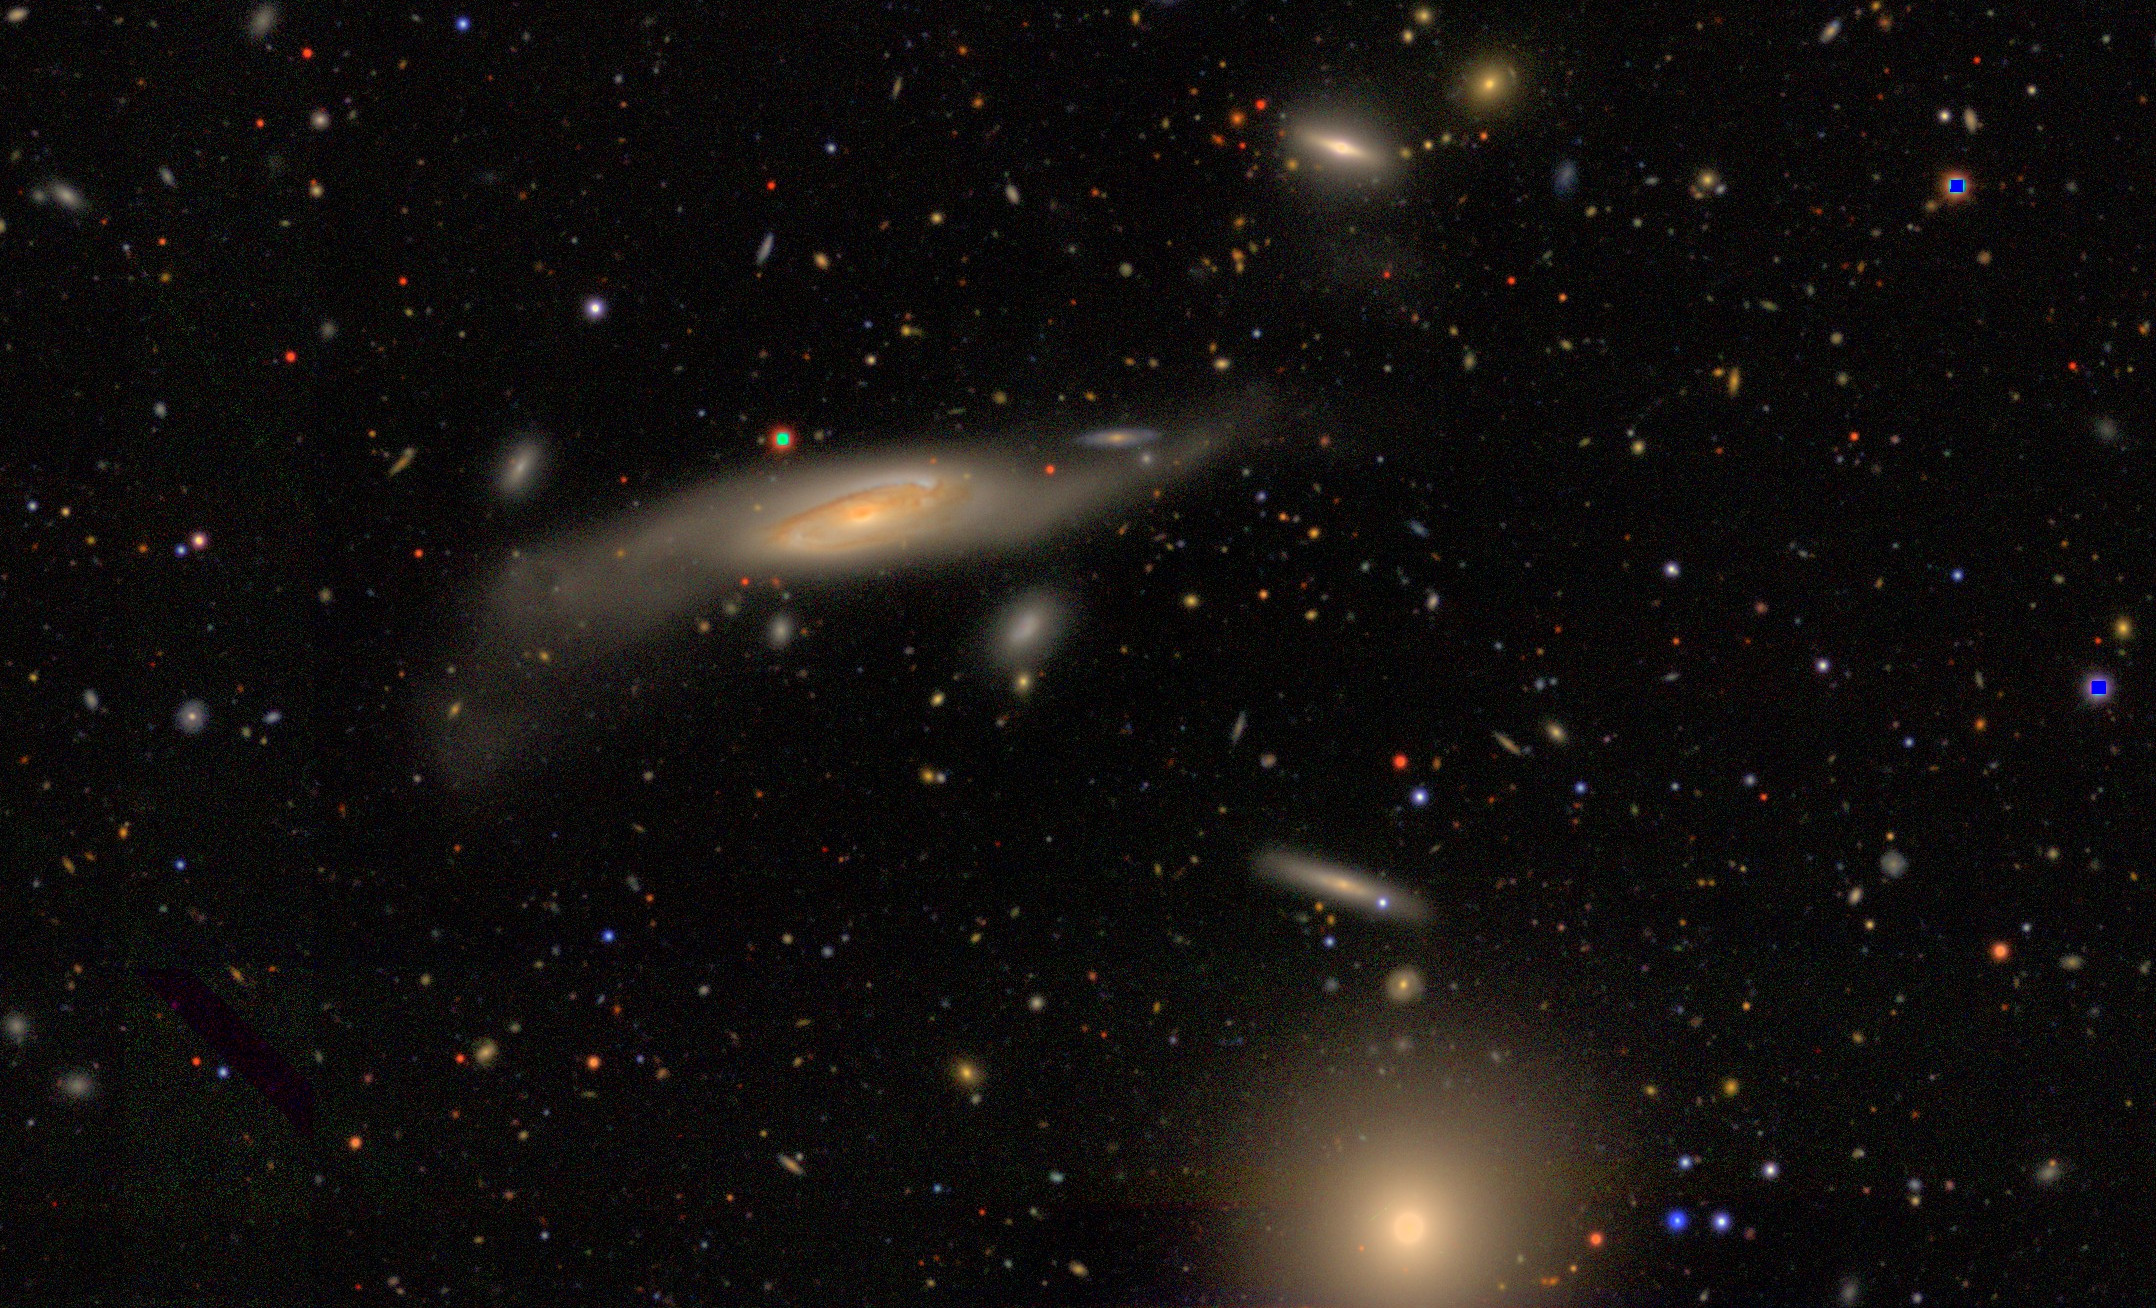
\includegraphics[height=\paperheight]{DES0056-5248_gri_crop.jpg}}
\frame
{
}
\setbeamertemplate{background canvas}[vertical shading][bottom=mgray,top=mblack]



\frame{\titlepage}


\setbeamerfont*{itemize/enumerate body}{size=\Large}
\setbeamerfont*{itemize/enumerate subbody}{parent=itemize/enumerate body}
\setbeamerfont*{itemize/enumerate subsubbody}{parent=itemize/enumerate body}

\frame
{
    \frametitle{About This Lecture}


    \begin{itemize}

        \item Targeted at those who have no background
            in astrophysics or cosmology

        \item My goal is to introduce concepts and give some examples

        \item I will not explain any details

        \item I will not explain the difficulties involved with actually
            doing the work

        \item Feel free to ask questions, {\em I don't care if I get through the
            material}

    \end{itemize}

}



\frame
{
    \frametitle{Outline}


    \begin{itemize}

        \item Brief introduction to cosmology
        \item Optical astronomy
        \item How we learn about cosmology with optical astronomy
        \item Two examples

    \end{itemize}

}

\frame
{

    {\huge Cosmology}

}

\frame
{
    \frametitle{Introduction to Cosmology}


    \begin{itemize}

        \item What makes up the universe? What can we see?

        \item Where is it all?  How is matter distributed?

        \item What is the history of the universe?

        \item Can we explain what we see?  Is what we see consistent with our
            understanding of fundamental physics?

    \end{itemize}

}


\frame
{

    \frametitle{What Makes Up the Universe?}

    \setbeamerfont*{itemize/enumerate body}{size=\large}

    \begin{columns}
        \begin{column}{0.5\textwidth}
            \begin{itemize}


                \item Particles -- people -- planets -- stars -- galaxies

                \item What is the composition of distant objects?

                \item What is the mass density of the universe?

                \item What fraction of the mass in the universe
                    is dark matter?

            \end{itemize}
        \end{column}
        \begin{column}{0.5\textwidth}
            \begin{center}
                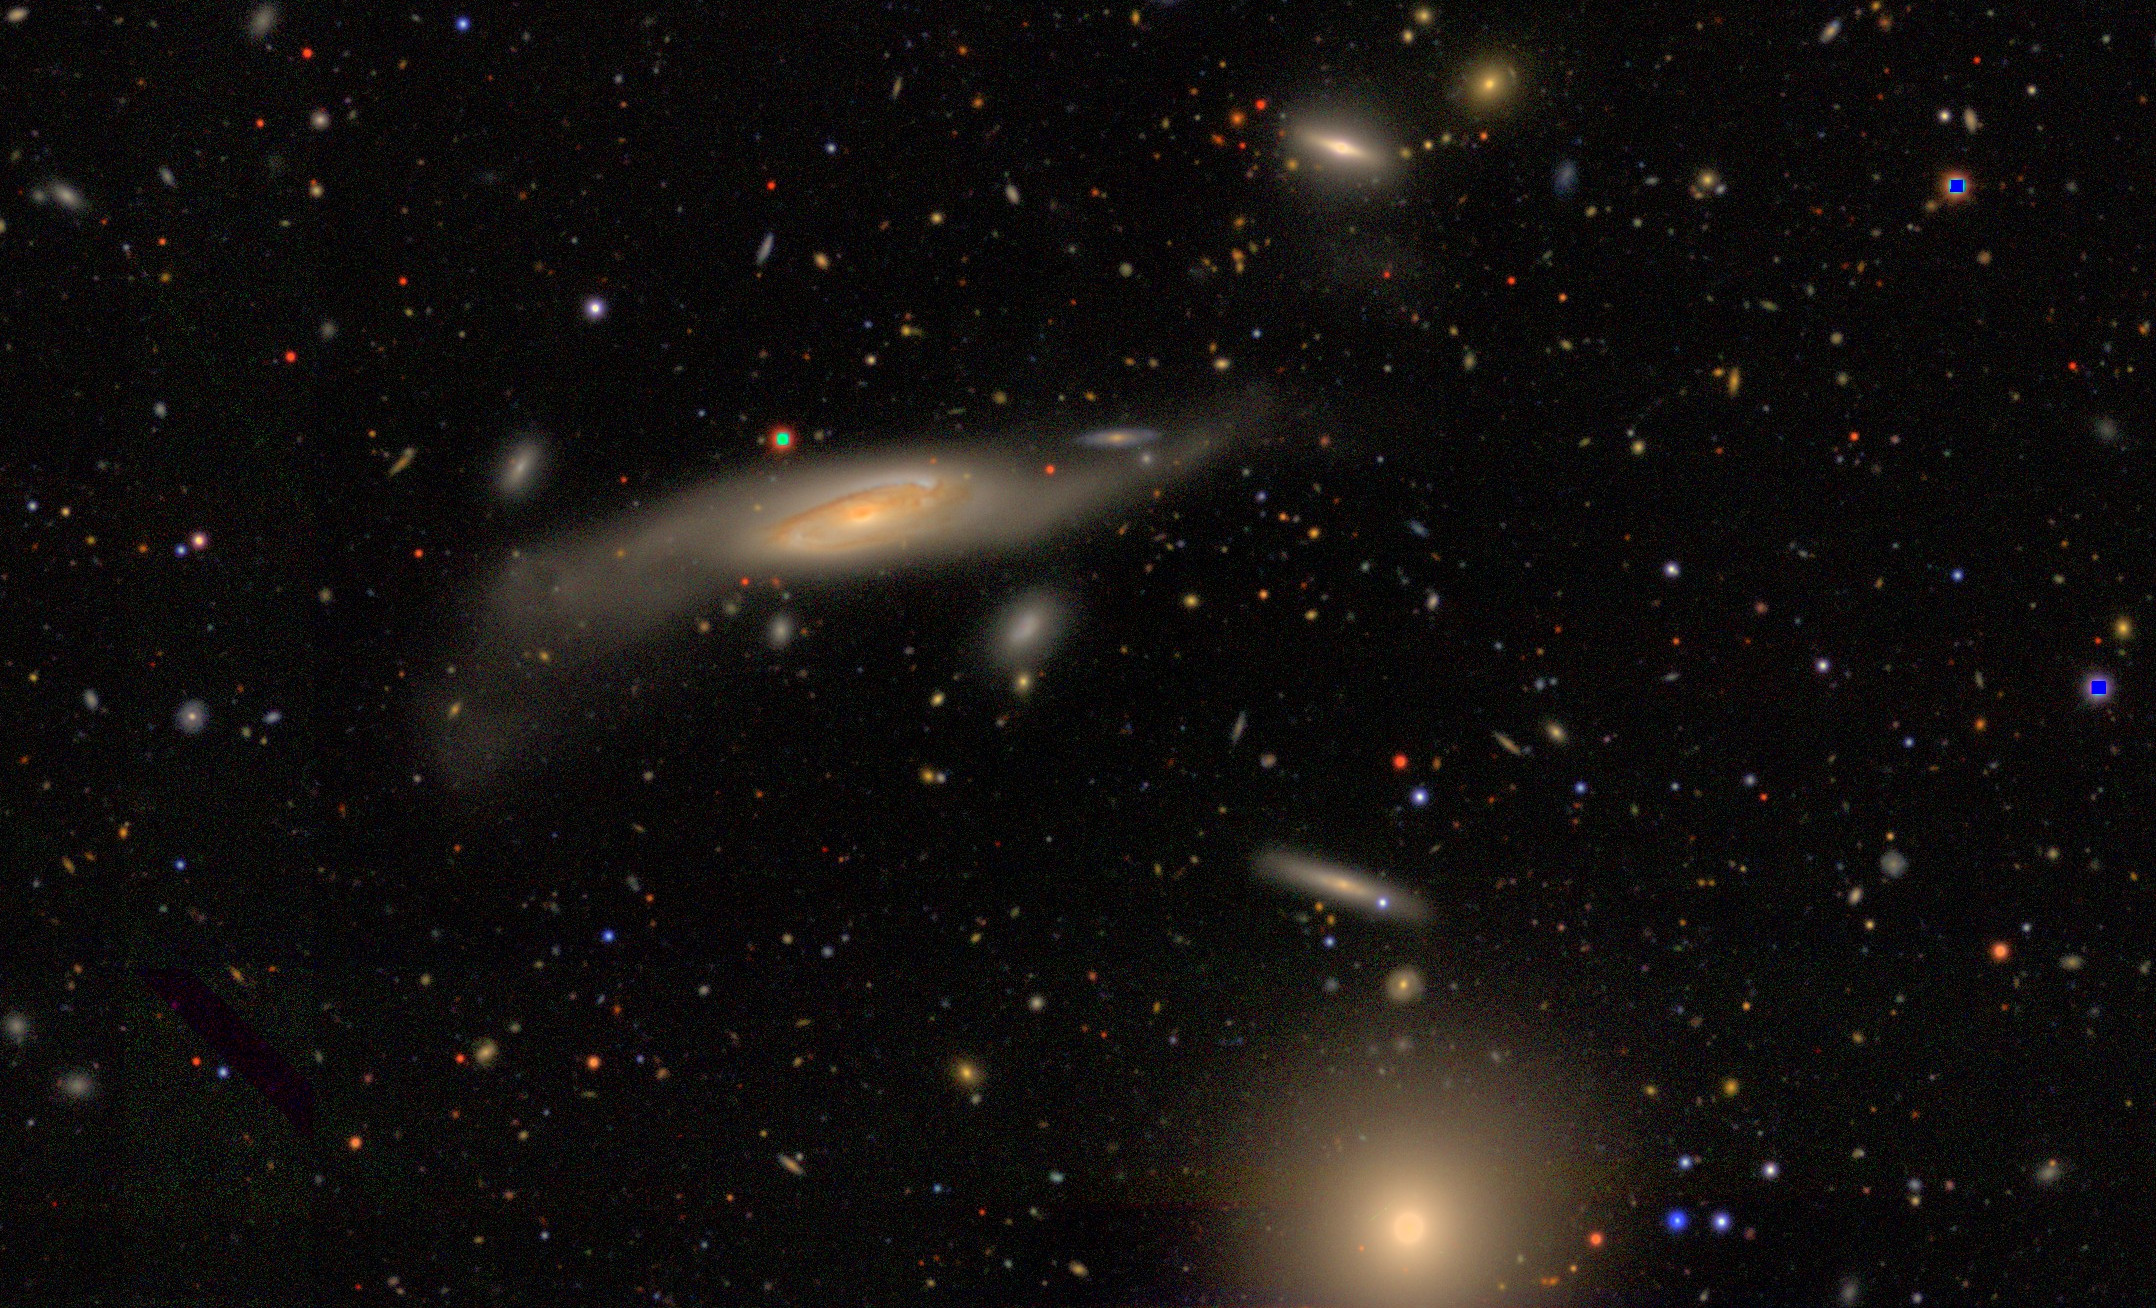
\includegraphics[width=1.2\textwidth, angle=90]{DES0056-5248_gri_crop.jpg}
                \newline
                {\tiny DES/Erin Sheldon}
            \end{center}
        \end{column}
    \end{columns}


}

\usebackgroundtemplate{%
    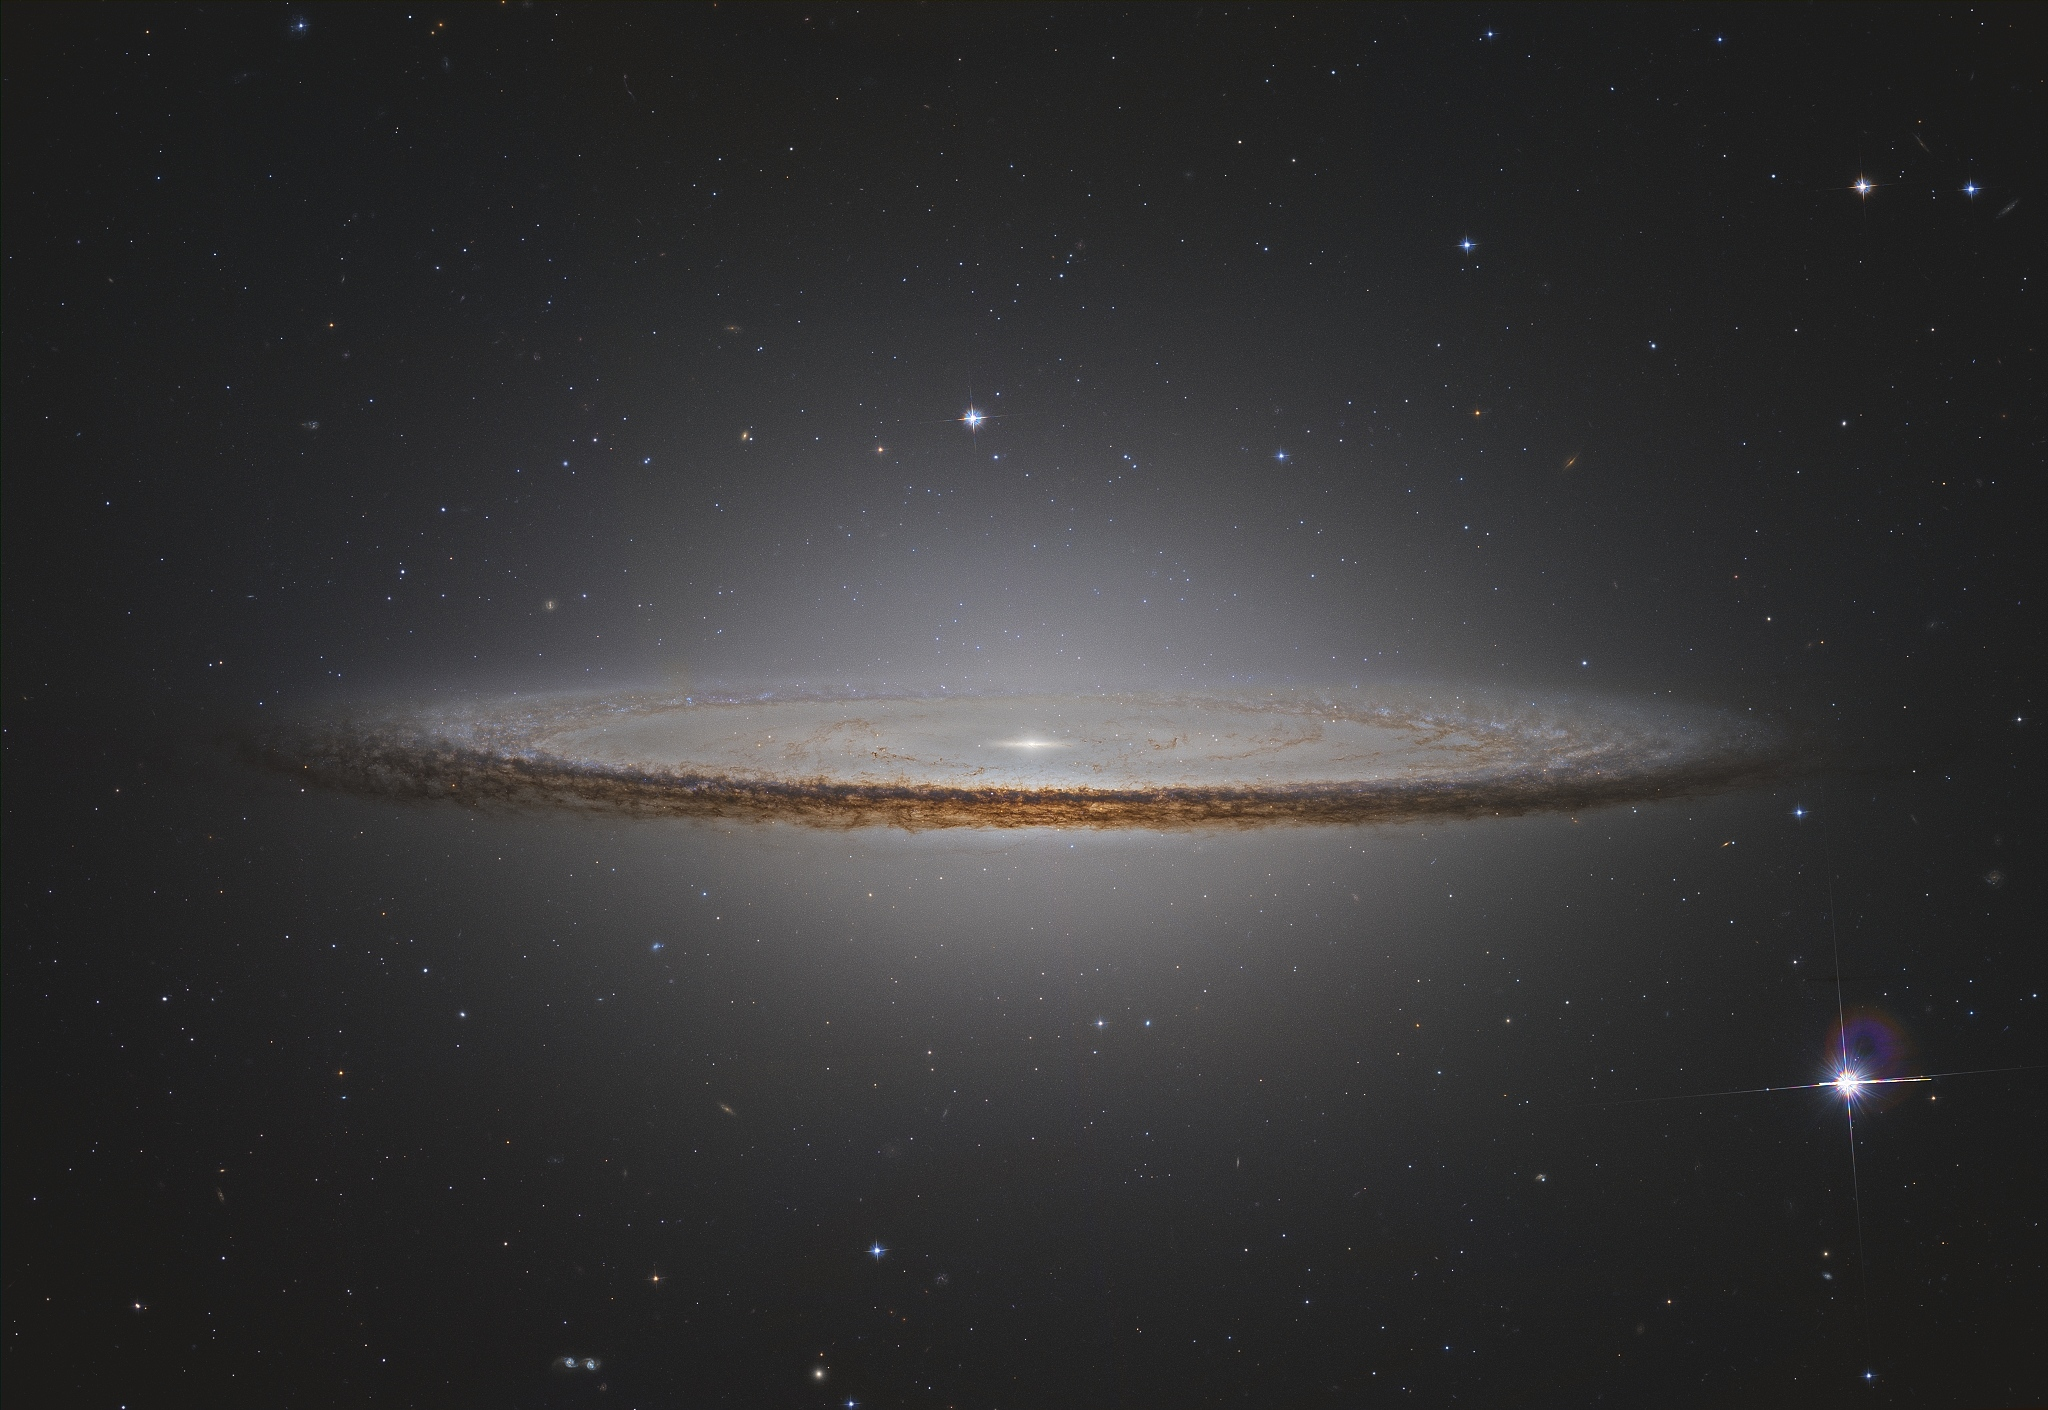
\includegraphics[width=\paperwidth,height=\paperheight]{M104b_peris2048.jpg}
}
\frame
{
}
\setbeamertemplate{background canvas}[vertical shading][bottom=mgray,top=mblack]


\frame
{

    \frametitle{How is matter distributed?}

    \setbeamerfont*{itemize/enumerate body}{size=\large}

    \begin{columns}
        \begin{column}{0.5\textwidth}
            \begin{itemize}


                \item Where are the stars and dark matter in our galaxy?

                \item Where are the galaxies and dark matter in the universe,
                    over large scales?


            \end{itemize}
        \end{column}
        \begin{column}{0.5\textwidth}
            \begin{center}
                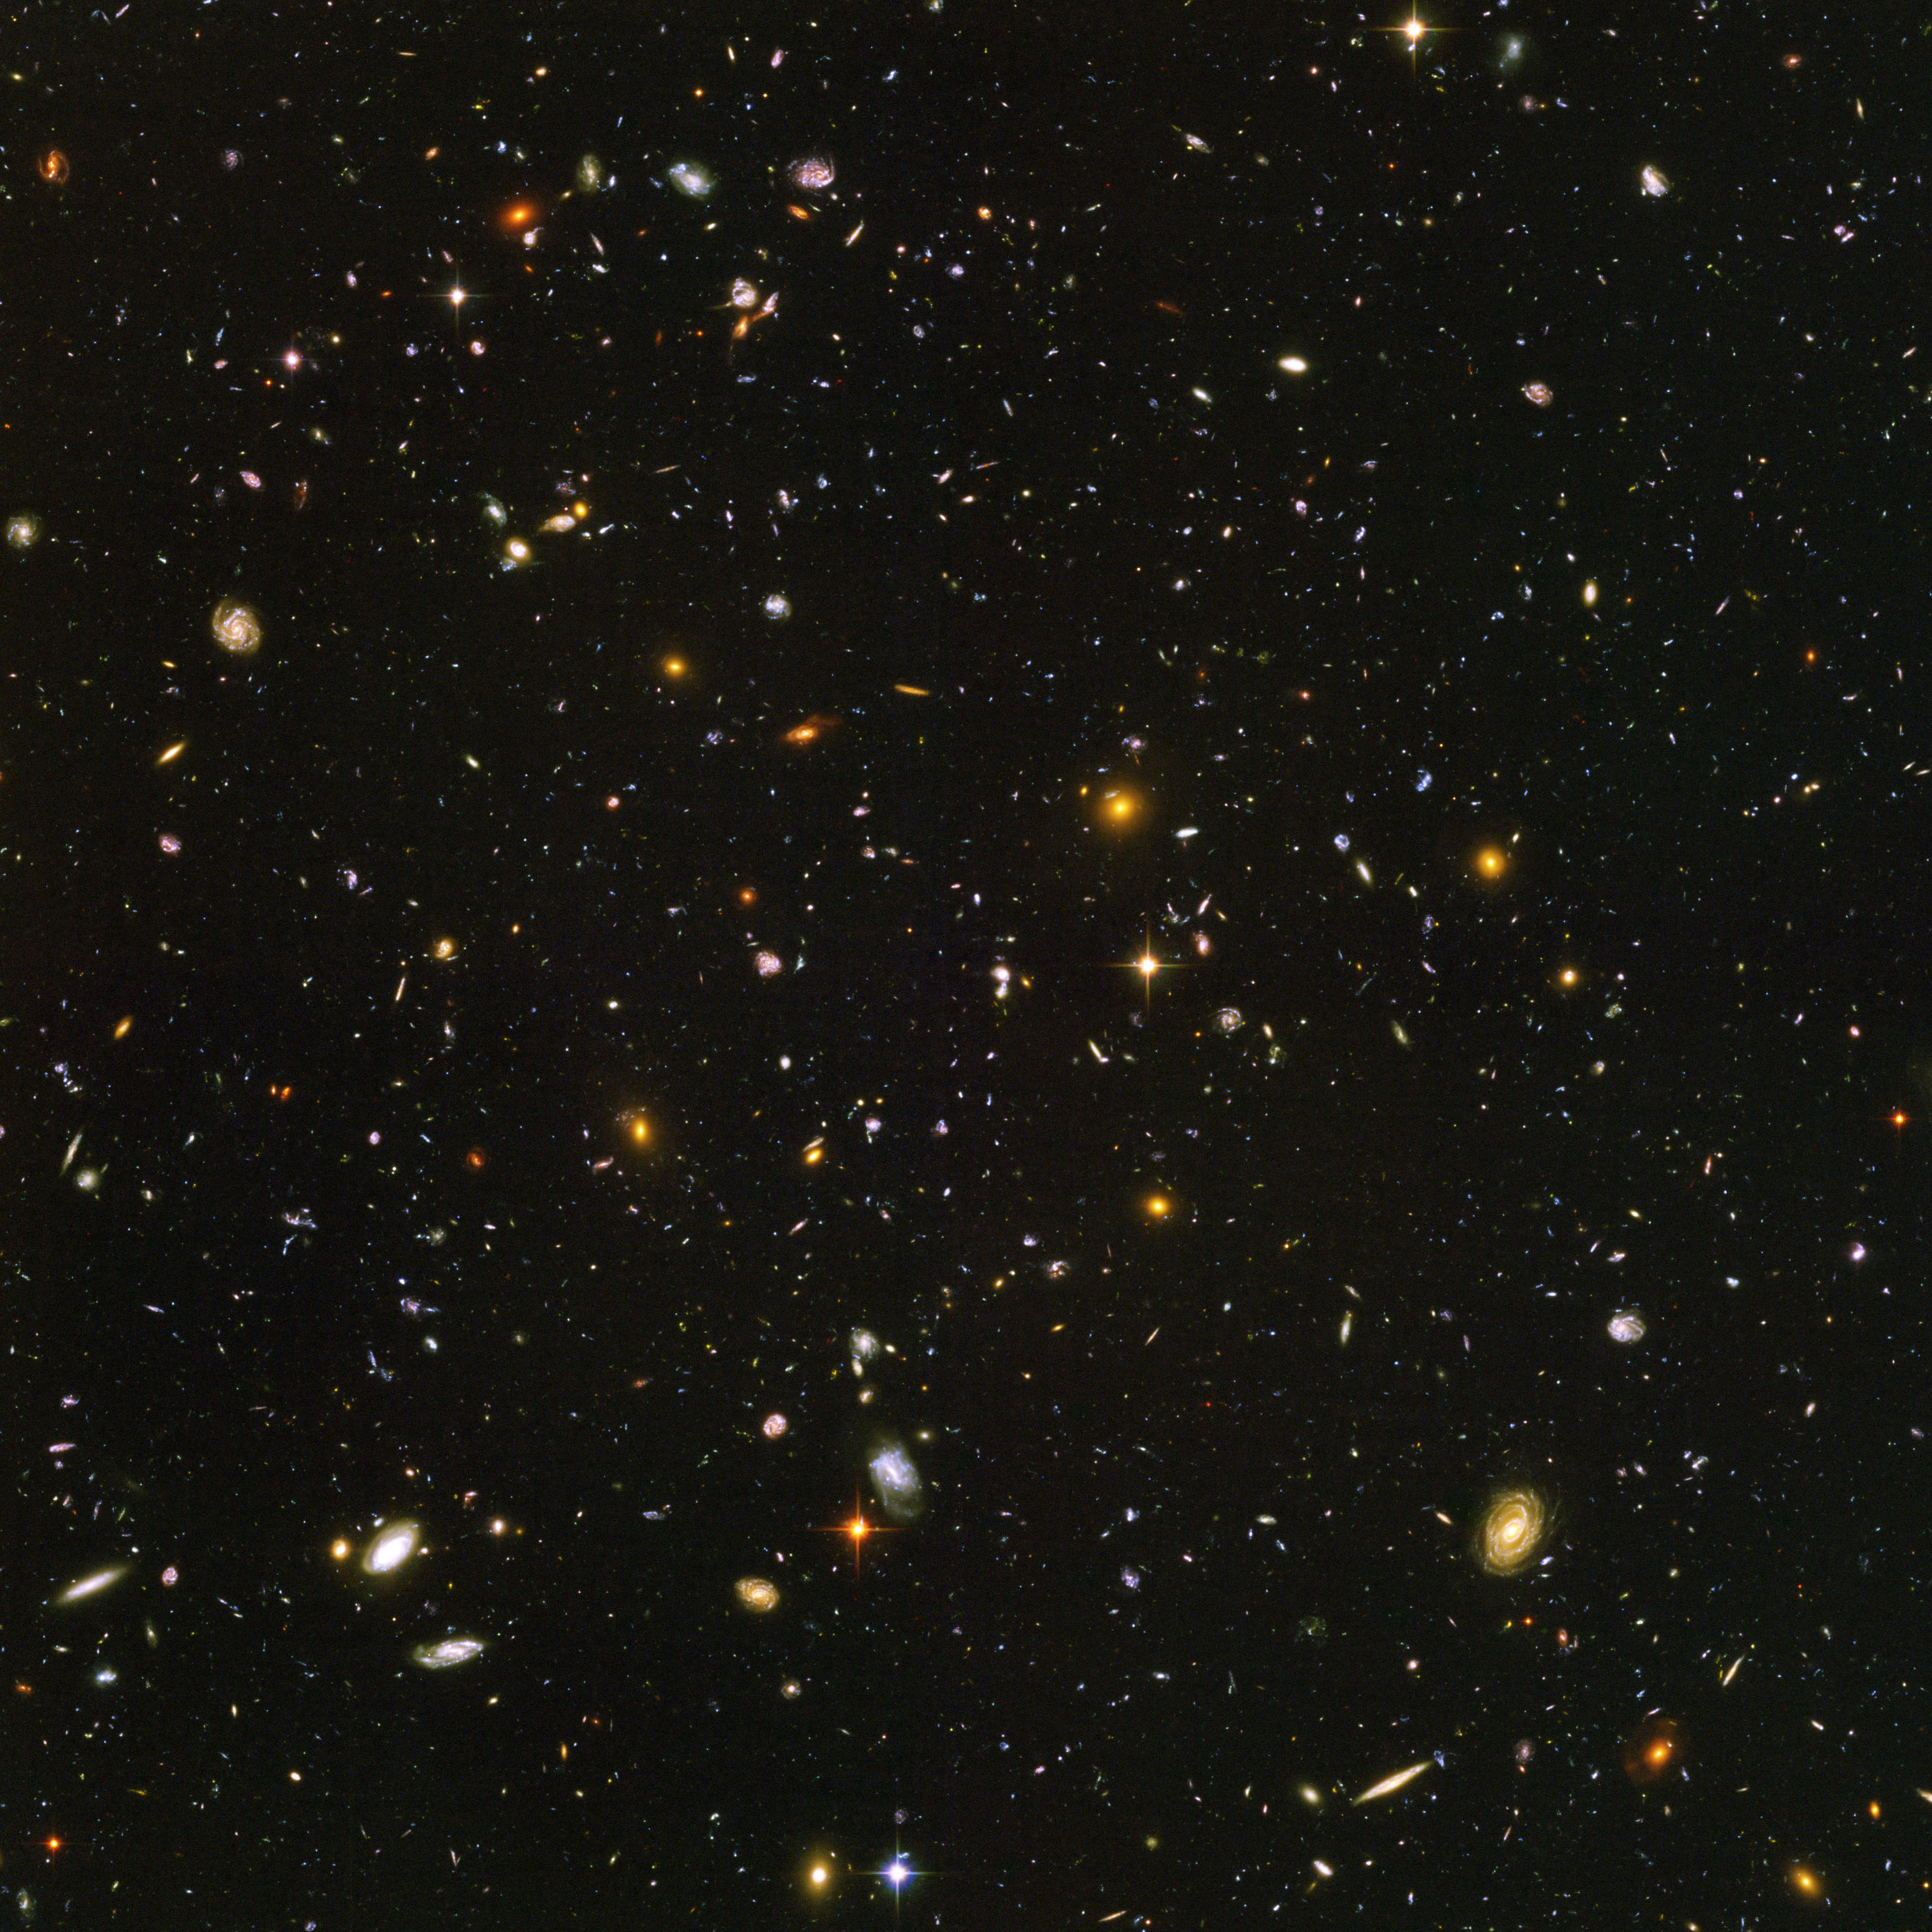
\includegraphics[width=\textwidth]{UDF_half.jpg}
            \end{center}
        \end{column}
    \end{columns}


}

\frame
{
    \begin{center}
        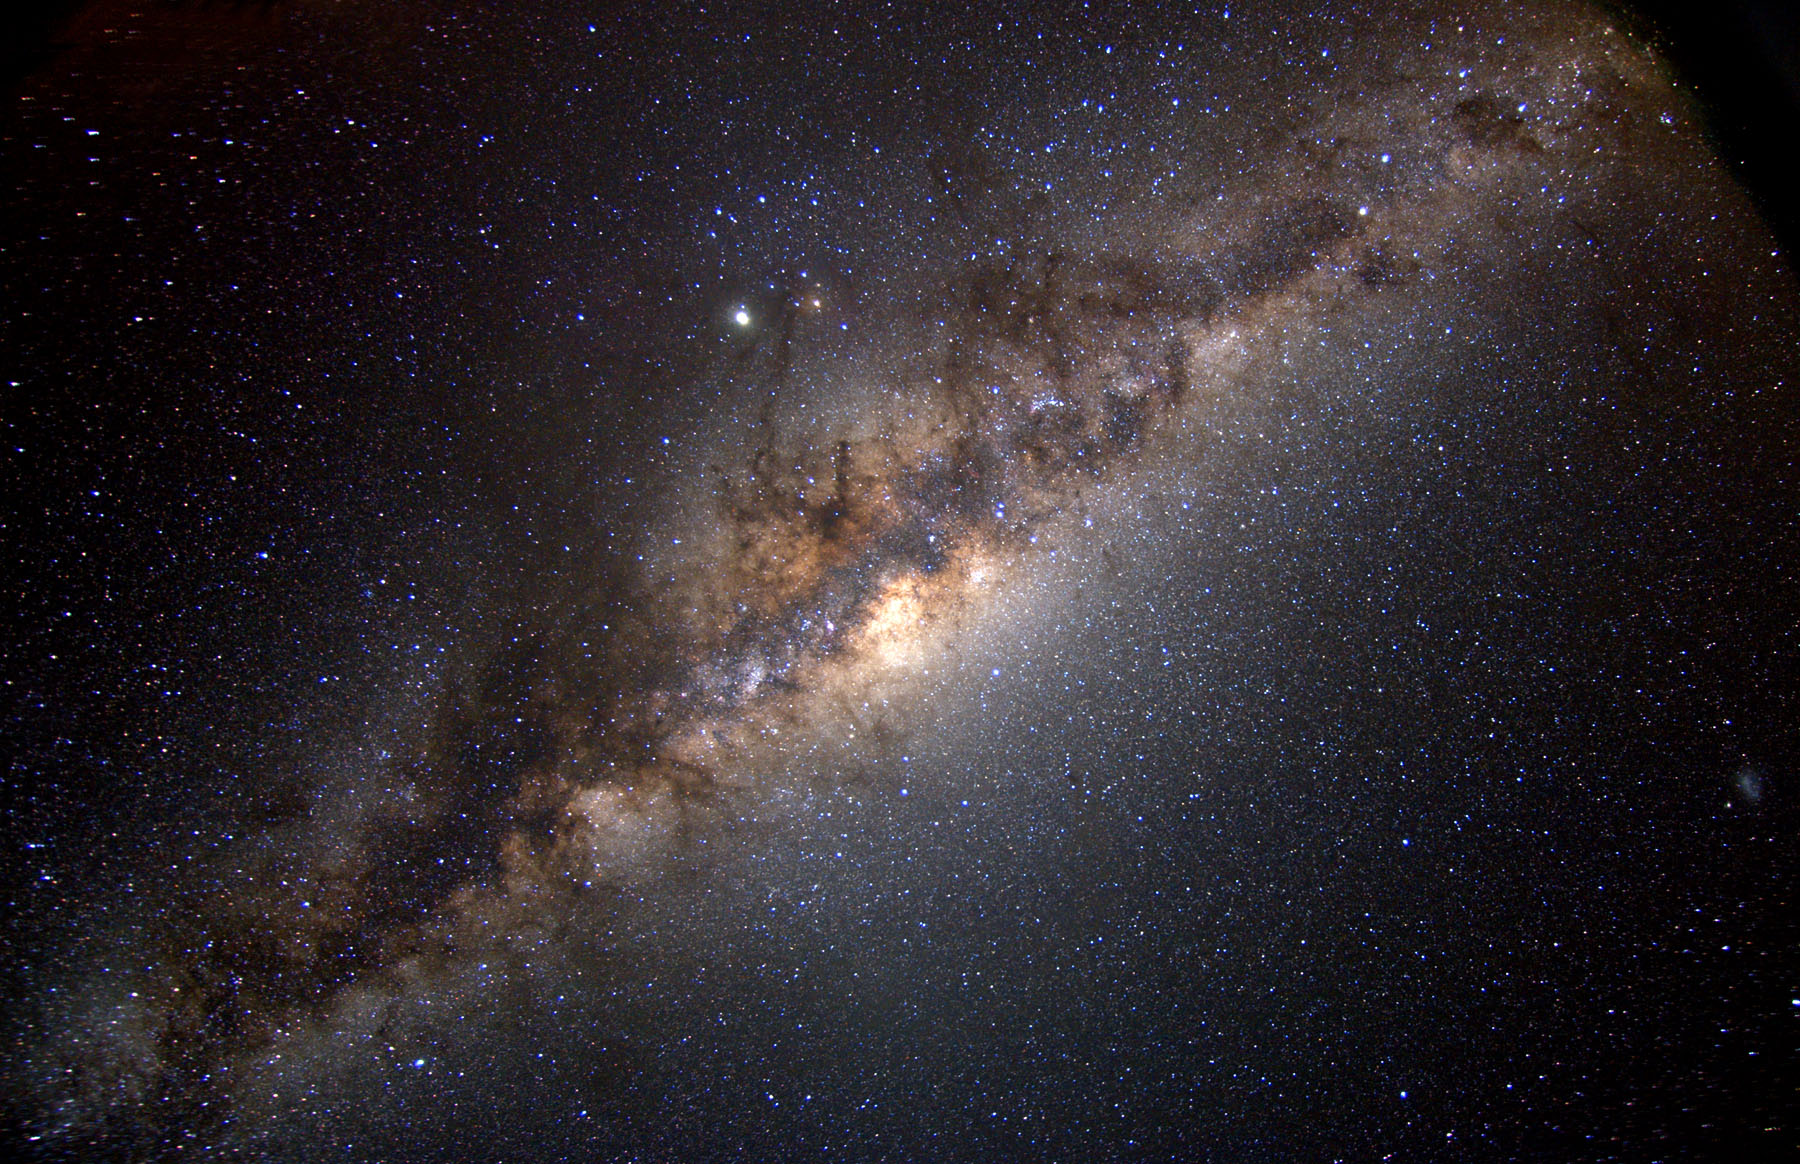
\includegraphics[width=0.95\textwidth]{16500feetmilkywaykc2_brunier.jpg}
    \end{center}
    {\normalsize The Milky Way (Serge Brunier)}
}


\frame
{
    \begin{center}
        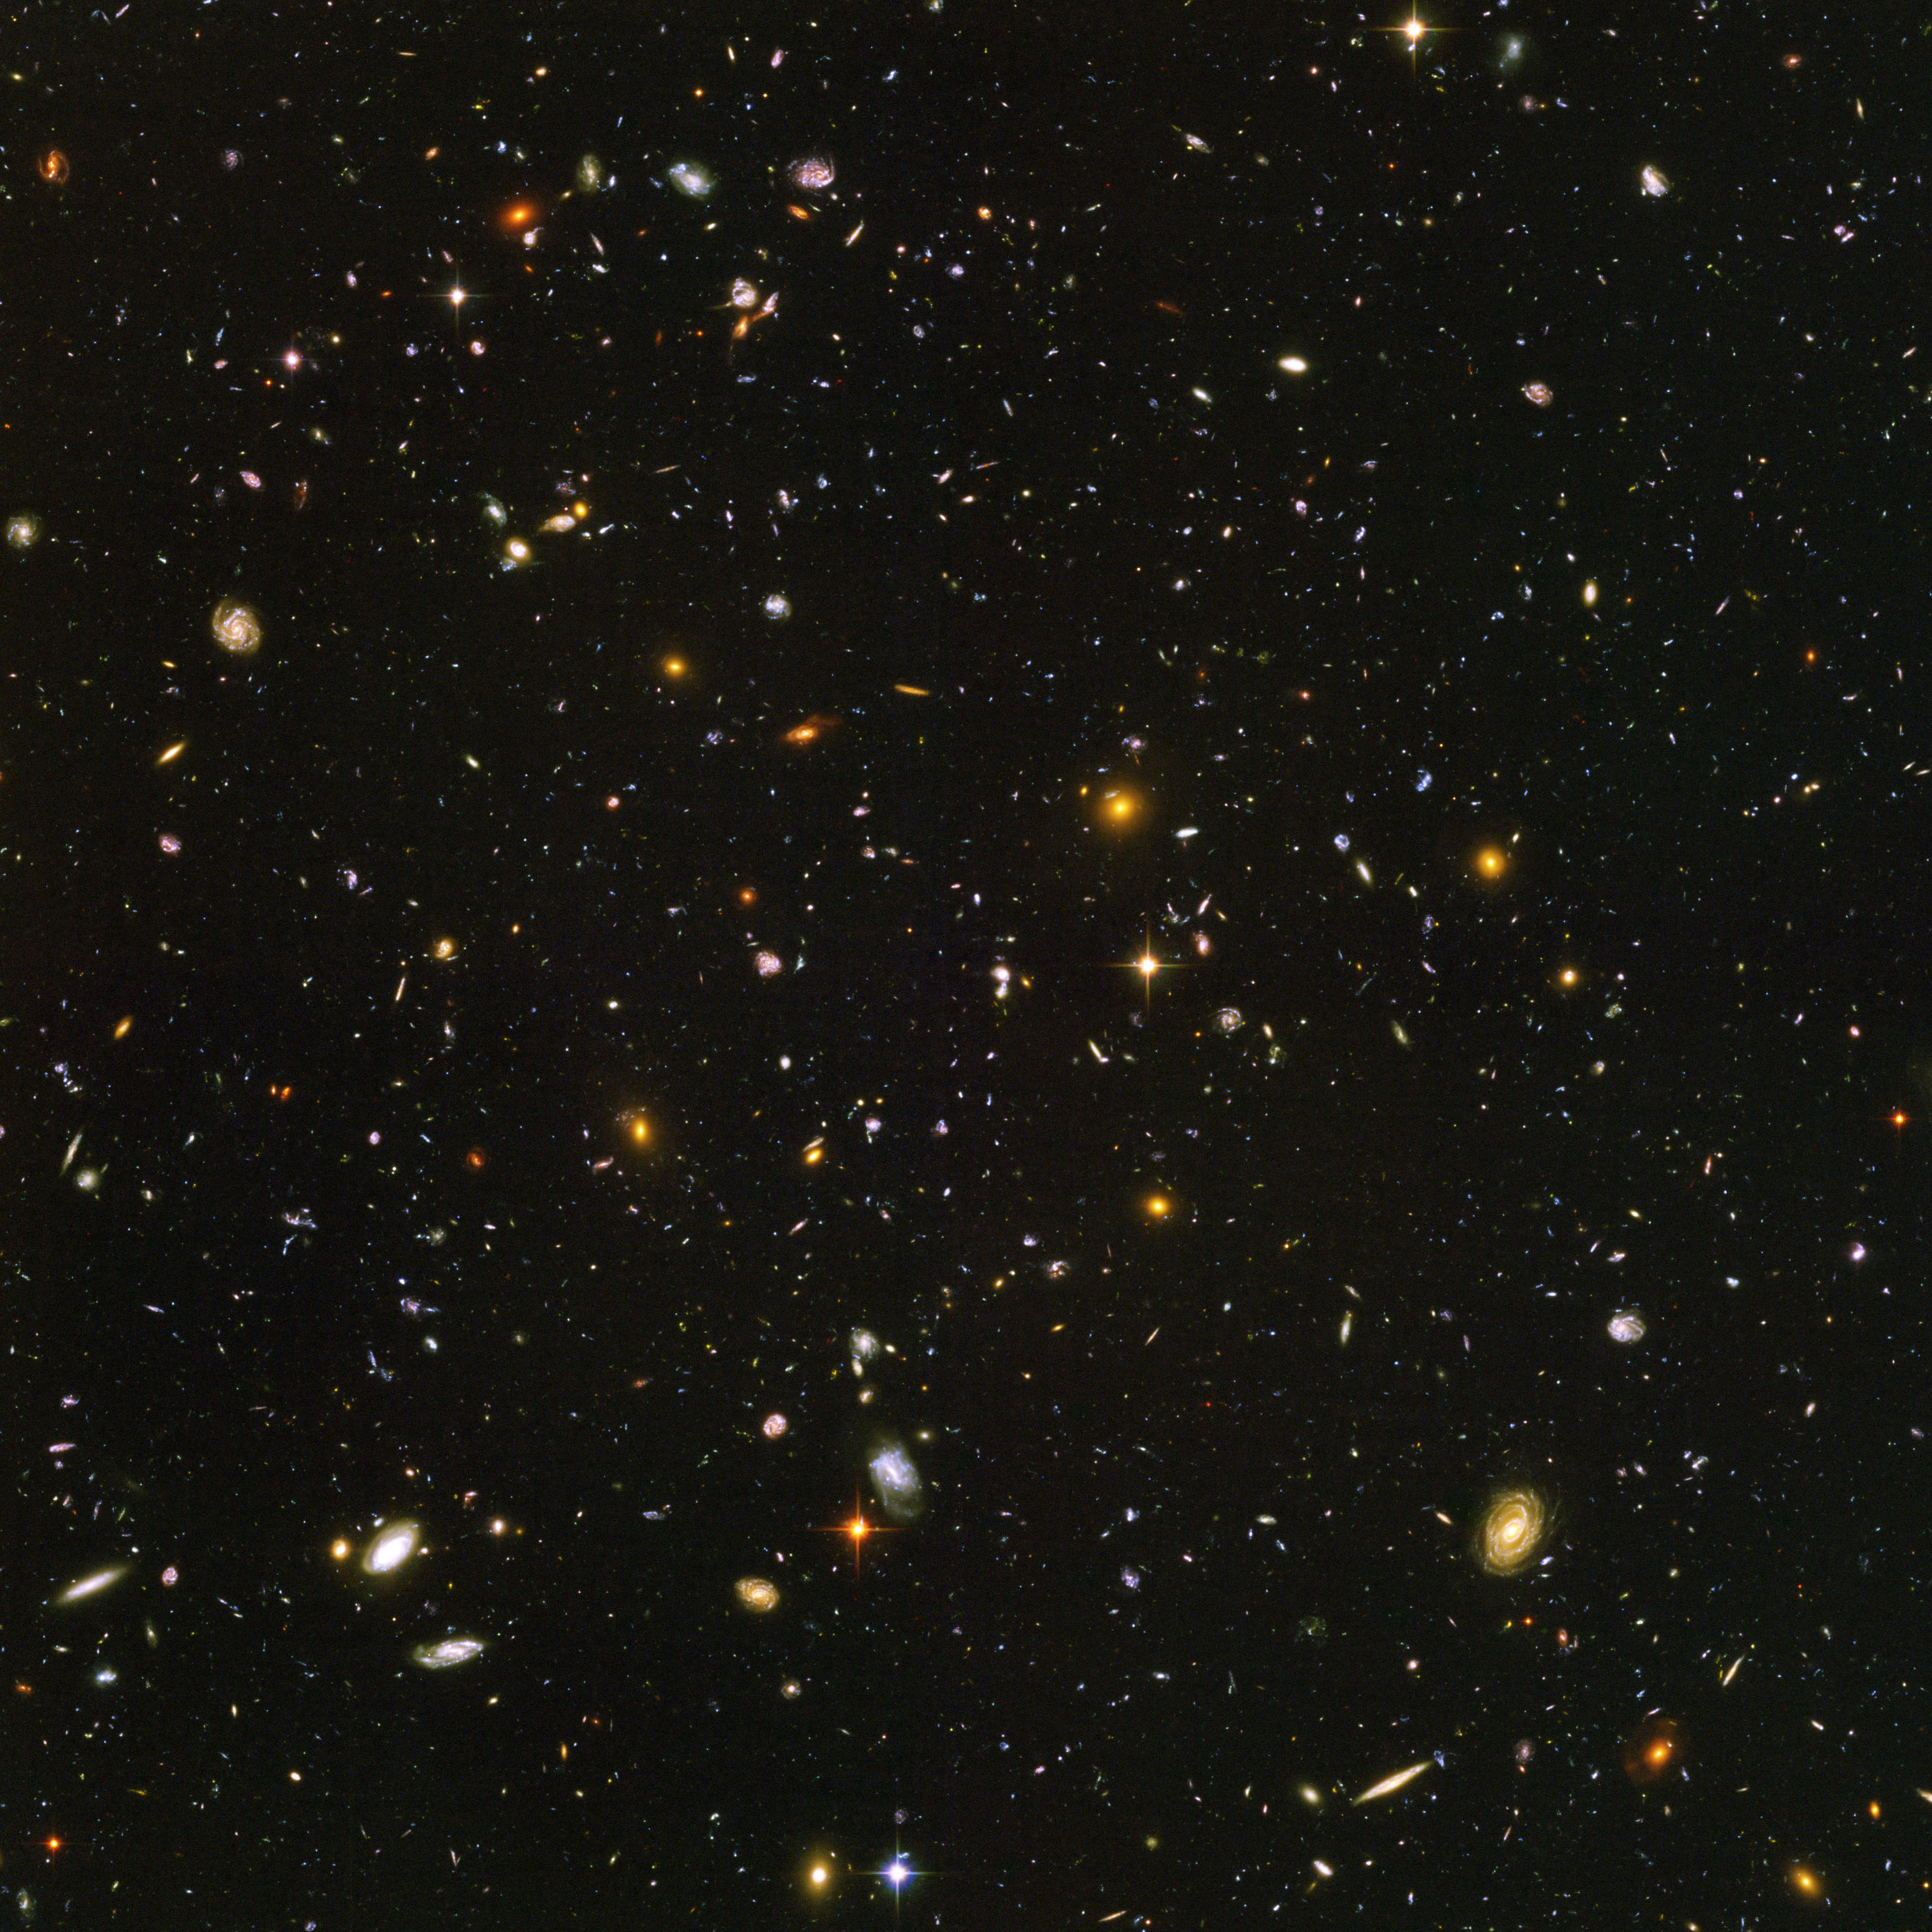
\includegraphics[width=0.8\textwidth]{UDF_half.jpg}
    \end{center}
    {\normalsize Hubble UDF}
}

\frame
{
    \begin{center}
        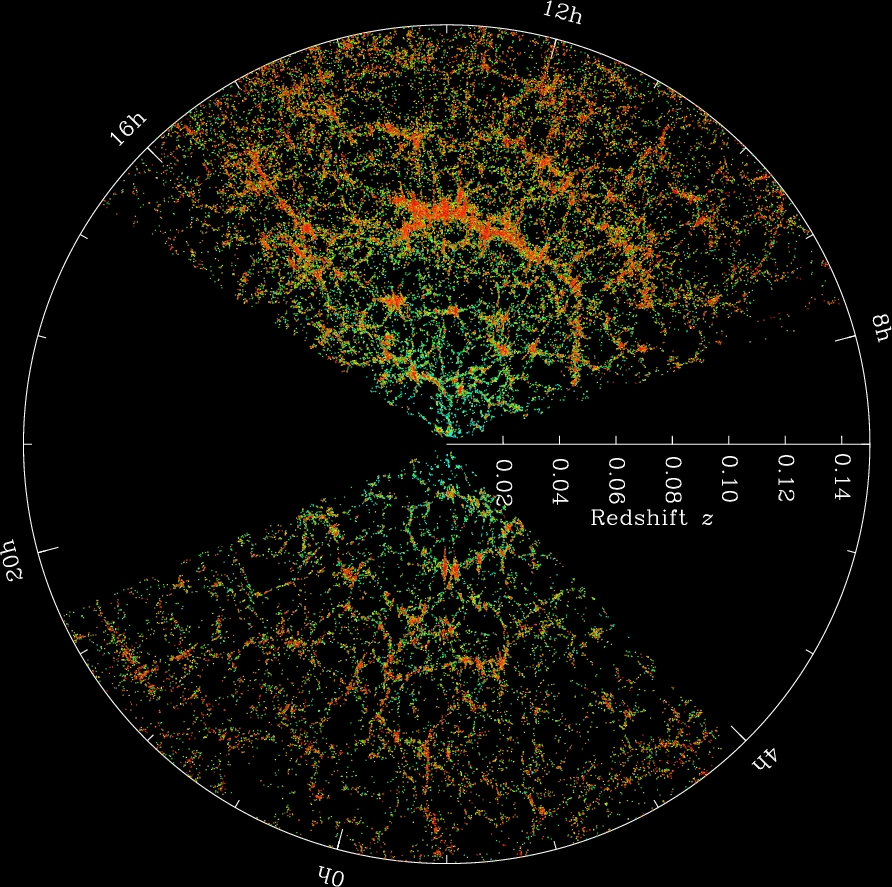
\includegraphics[height=0.9\textheight]{orangepie.jpg}
    \end{center}
    {\normalsize SDSS Galaxy Locations (M. Blanton)}
}


\frame
{

    \frametitle{What is the history of the universe?}

    \setbeamerfont*{itemize/enumerate body}{size=\small}

    \begin{columns}
        \begin{column}{0.5\textwidth}
            \begin{itemize}


                \item The universe is expanding.  Galaxies farther away from
                    us moving away faster and their light is redshifted
                    
                \item That is our view, but you would see the same thing
                    from any other galaxy in the universe

                \item We can get an estimate of distance from the
                    velocity/redshift.
                    
                \item Because we see these galaxies as they were far back in
                    time, the history is tied to the question of where things
                    are.

            \end{itemize}
        \end{column}
        \begin{column}{0.5\textwidth}
            \begin{center}
                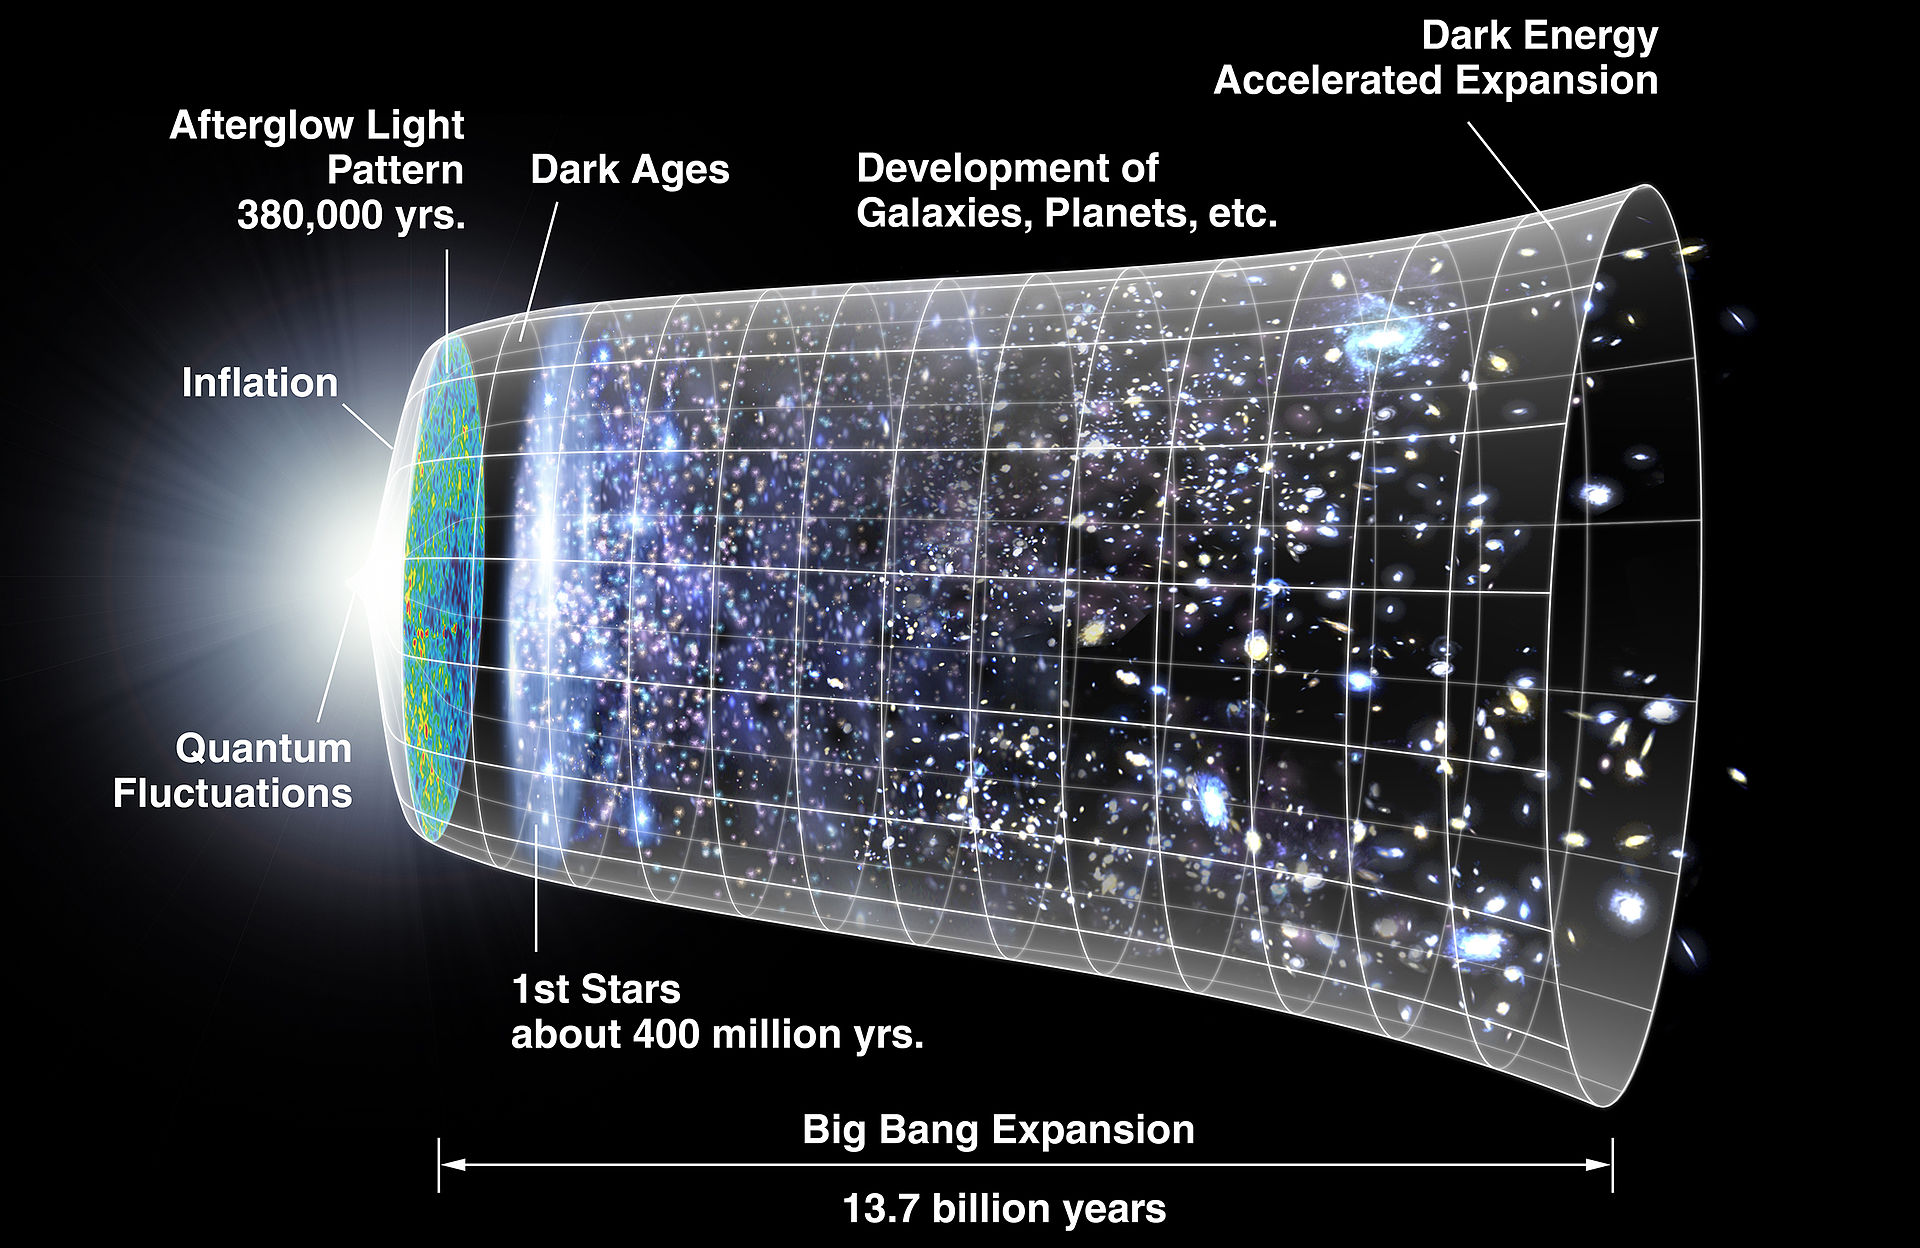
\includegraphics[width=\textwidth]{CMB_Timeline300_no_WMAP.jpg}
            \end{center}
            
        \end{column}
    \end{columns}


}

\frame
{

    \frametitle{What is the history of the universe?}

    \setbeamerfont*{itemize/enumerate body}{size=\small}

    \begin{columns}
        \begin{column}{0.5\textwidth}
            \begin{itemize}


                \item We expected the expansion to decelerate. 

                \item The measurements indicated it {\em did} decelerate for a
                    long time, but then began to accelerate!
                    
                \item This mystery is called Dark Energy 
                    

            \end{itemize}
        \end{column}
        \begin{column}{0.5\textwidth}
            \begin{center}
                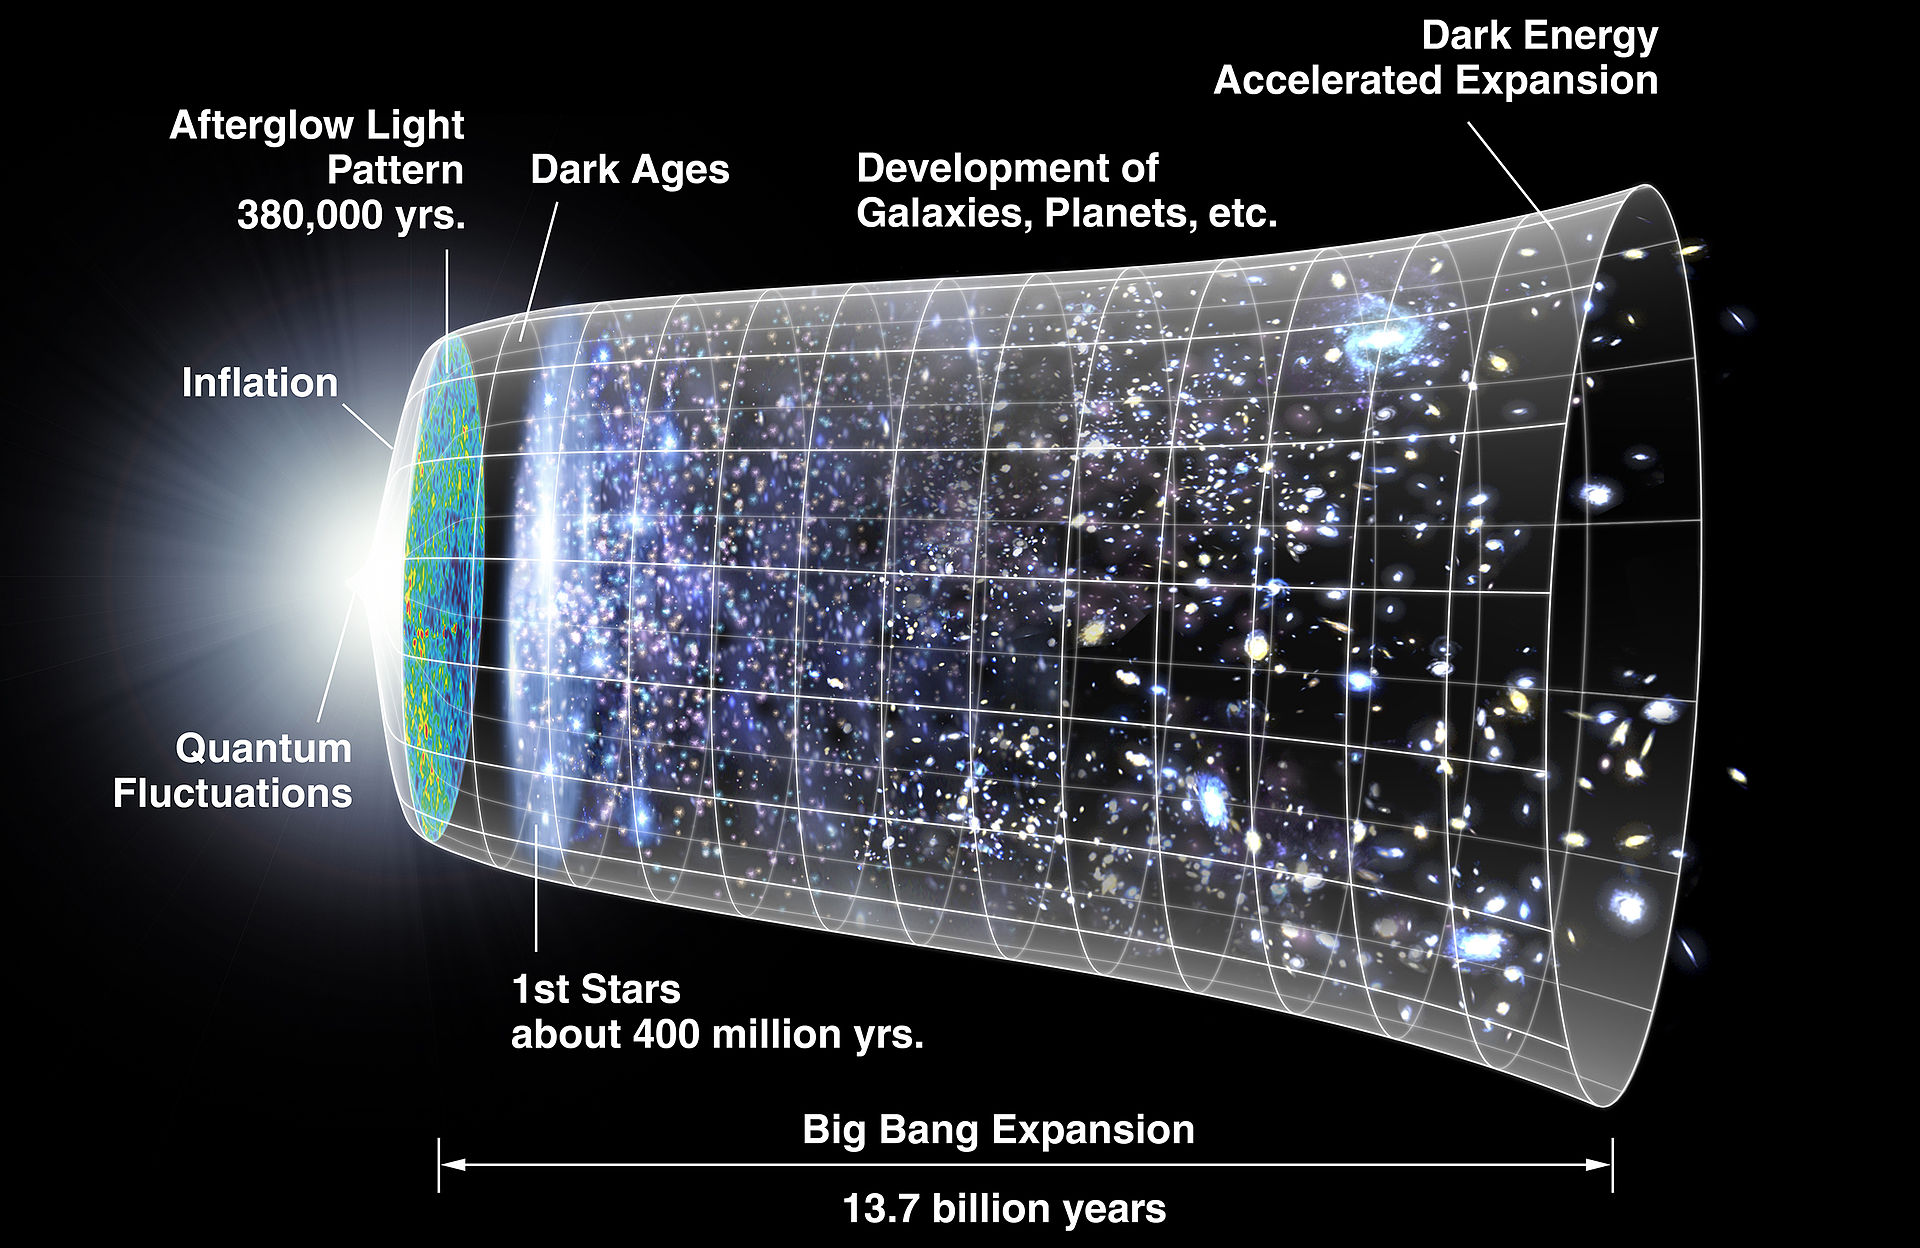
\includegraphics[width=\textwidth]{CMB_Timeline300_no_WMAP.jpg}
            \end{center}
            
        \end{column}
    \end{columns}


}

\frame
{
    \begin{center}
        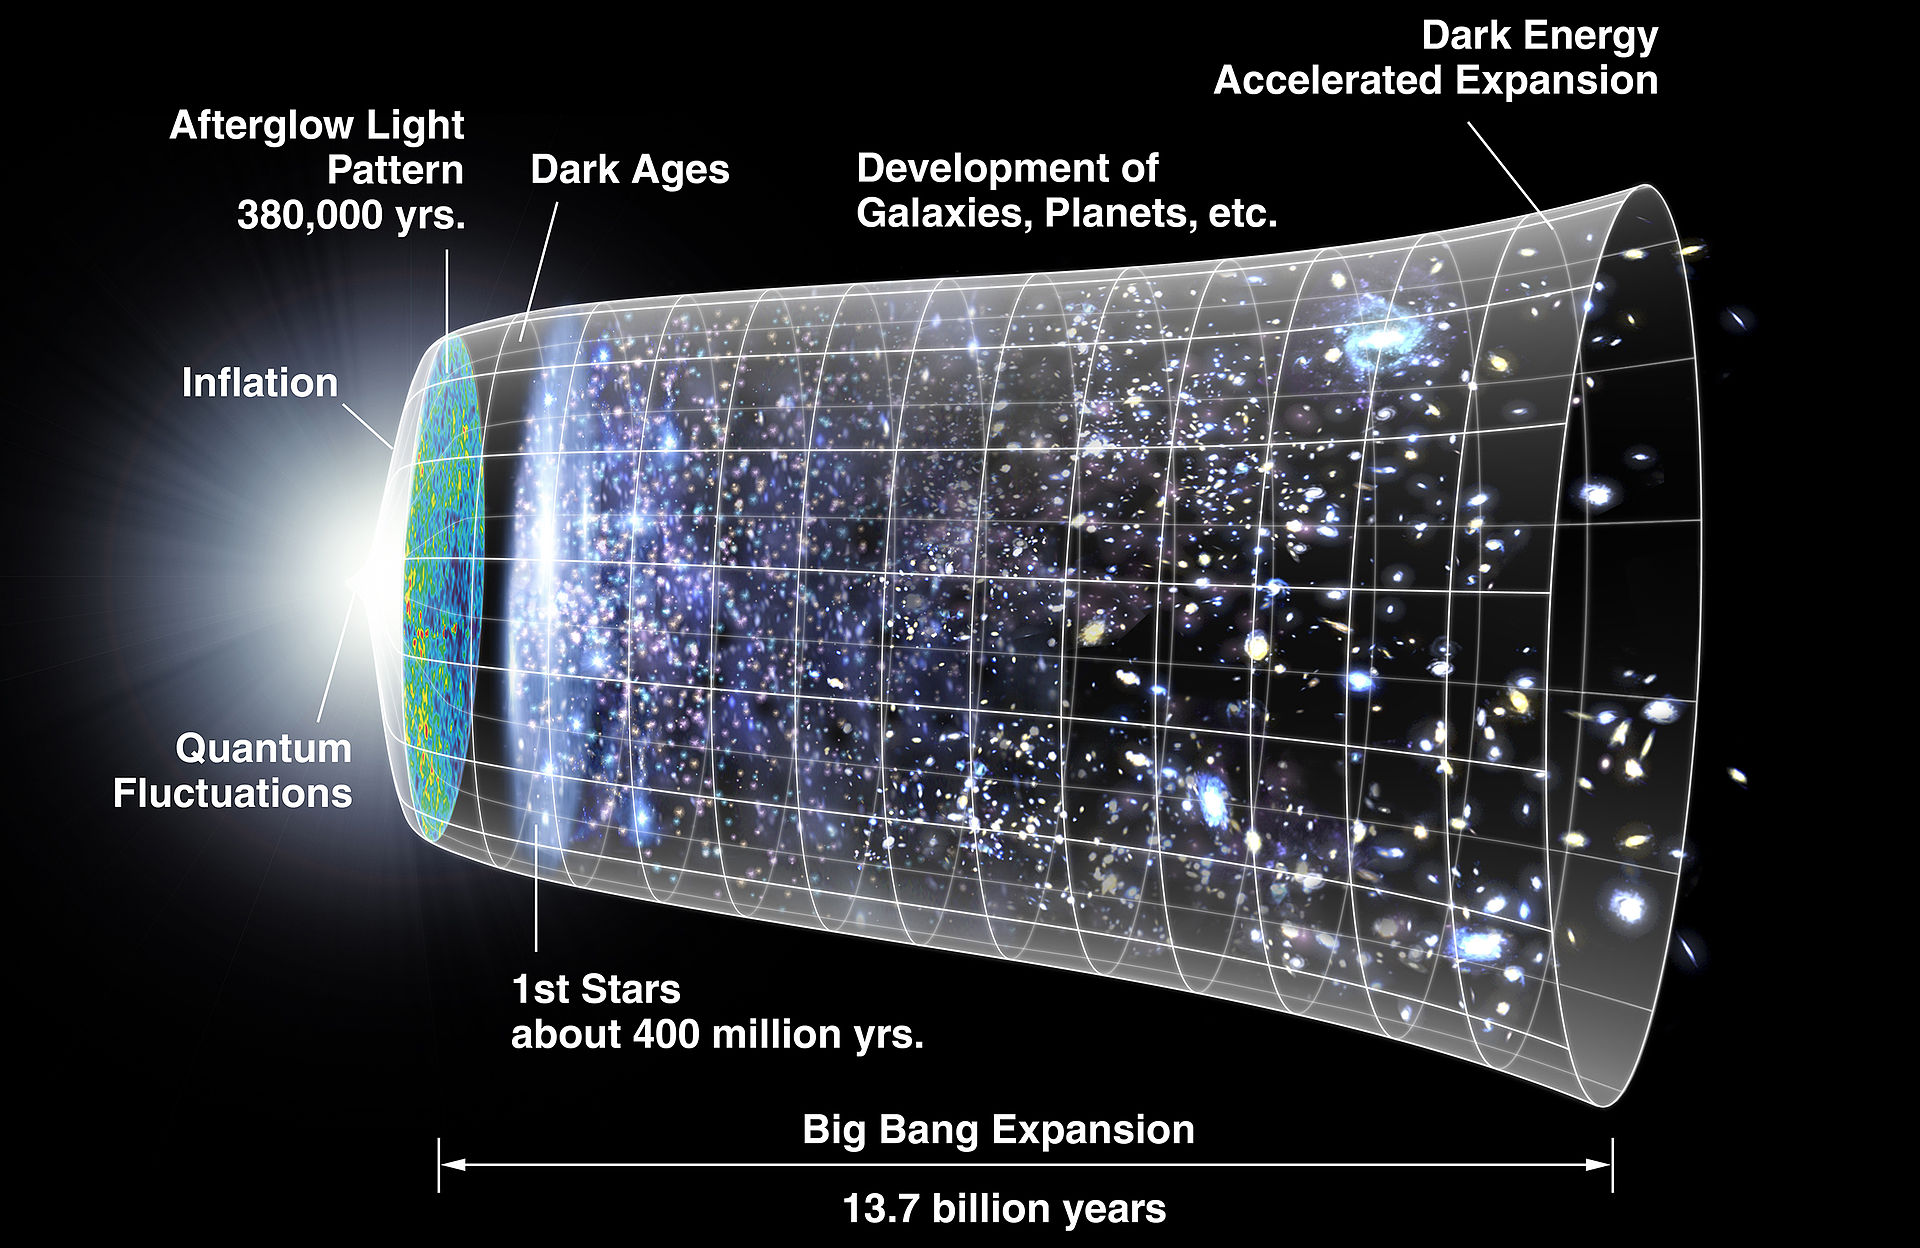
\includegraphics[width=0.9\textwidth]{CMB_Timeline300_no_WMAP.jpg}
    \end{center}
    {\normalsize Model of the expansion history (WMAP)}
}



\frame
{

    \frametitle{What is the history of the universe?}

    \setbeamerfont*{itemize/enumerate body}{size=\small}

    \begin{columns}
        \begin{column}{0.5\textwidth}
            \begin{itemize}

                \item There was some effective ``beginning'' when the universe
                    was extremely hot and dense.

                \item How did the visible universe evolve, from formation of
                    the first nuclei to stars to the large scale structure of
                    the universe?

            \end{itemize}
        \end{column}
        \begin{column}{0.5\textwidth}
            \begin{center}
                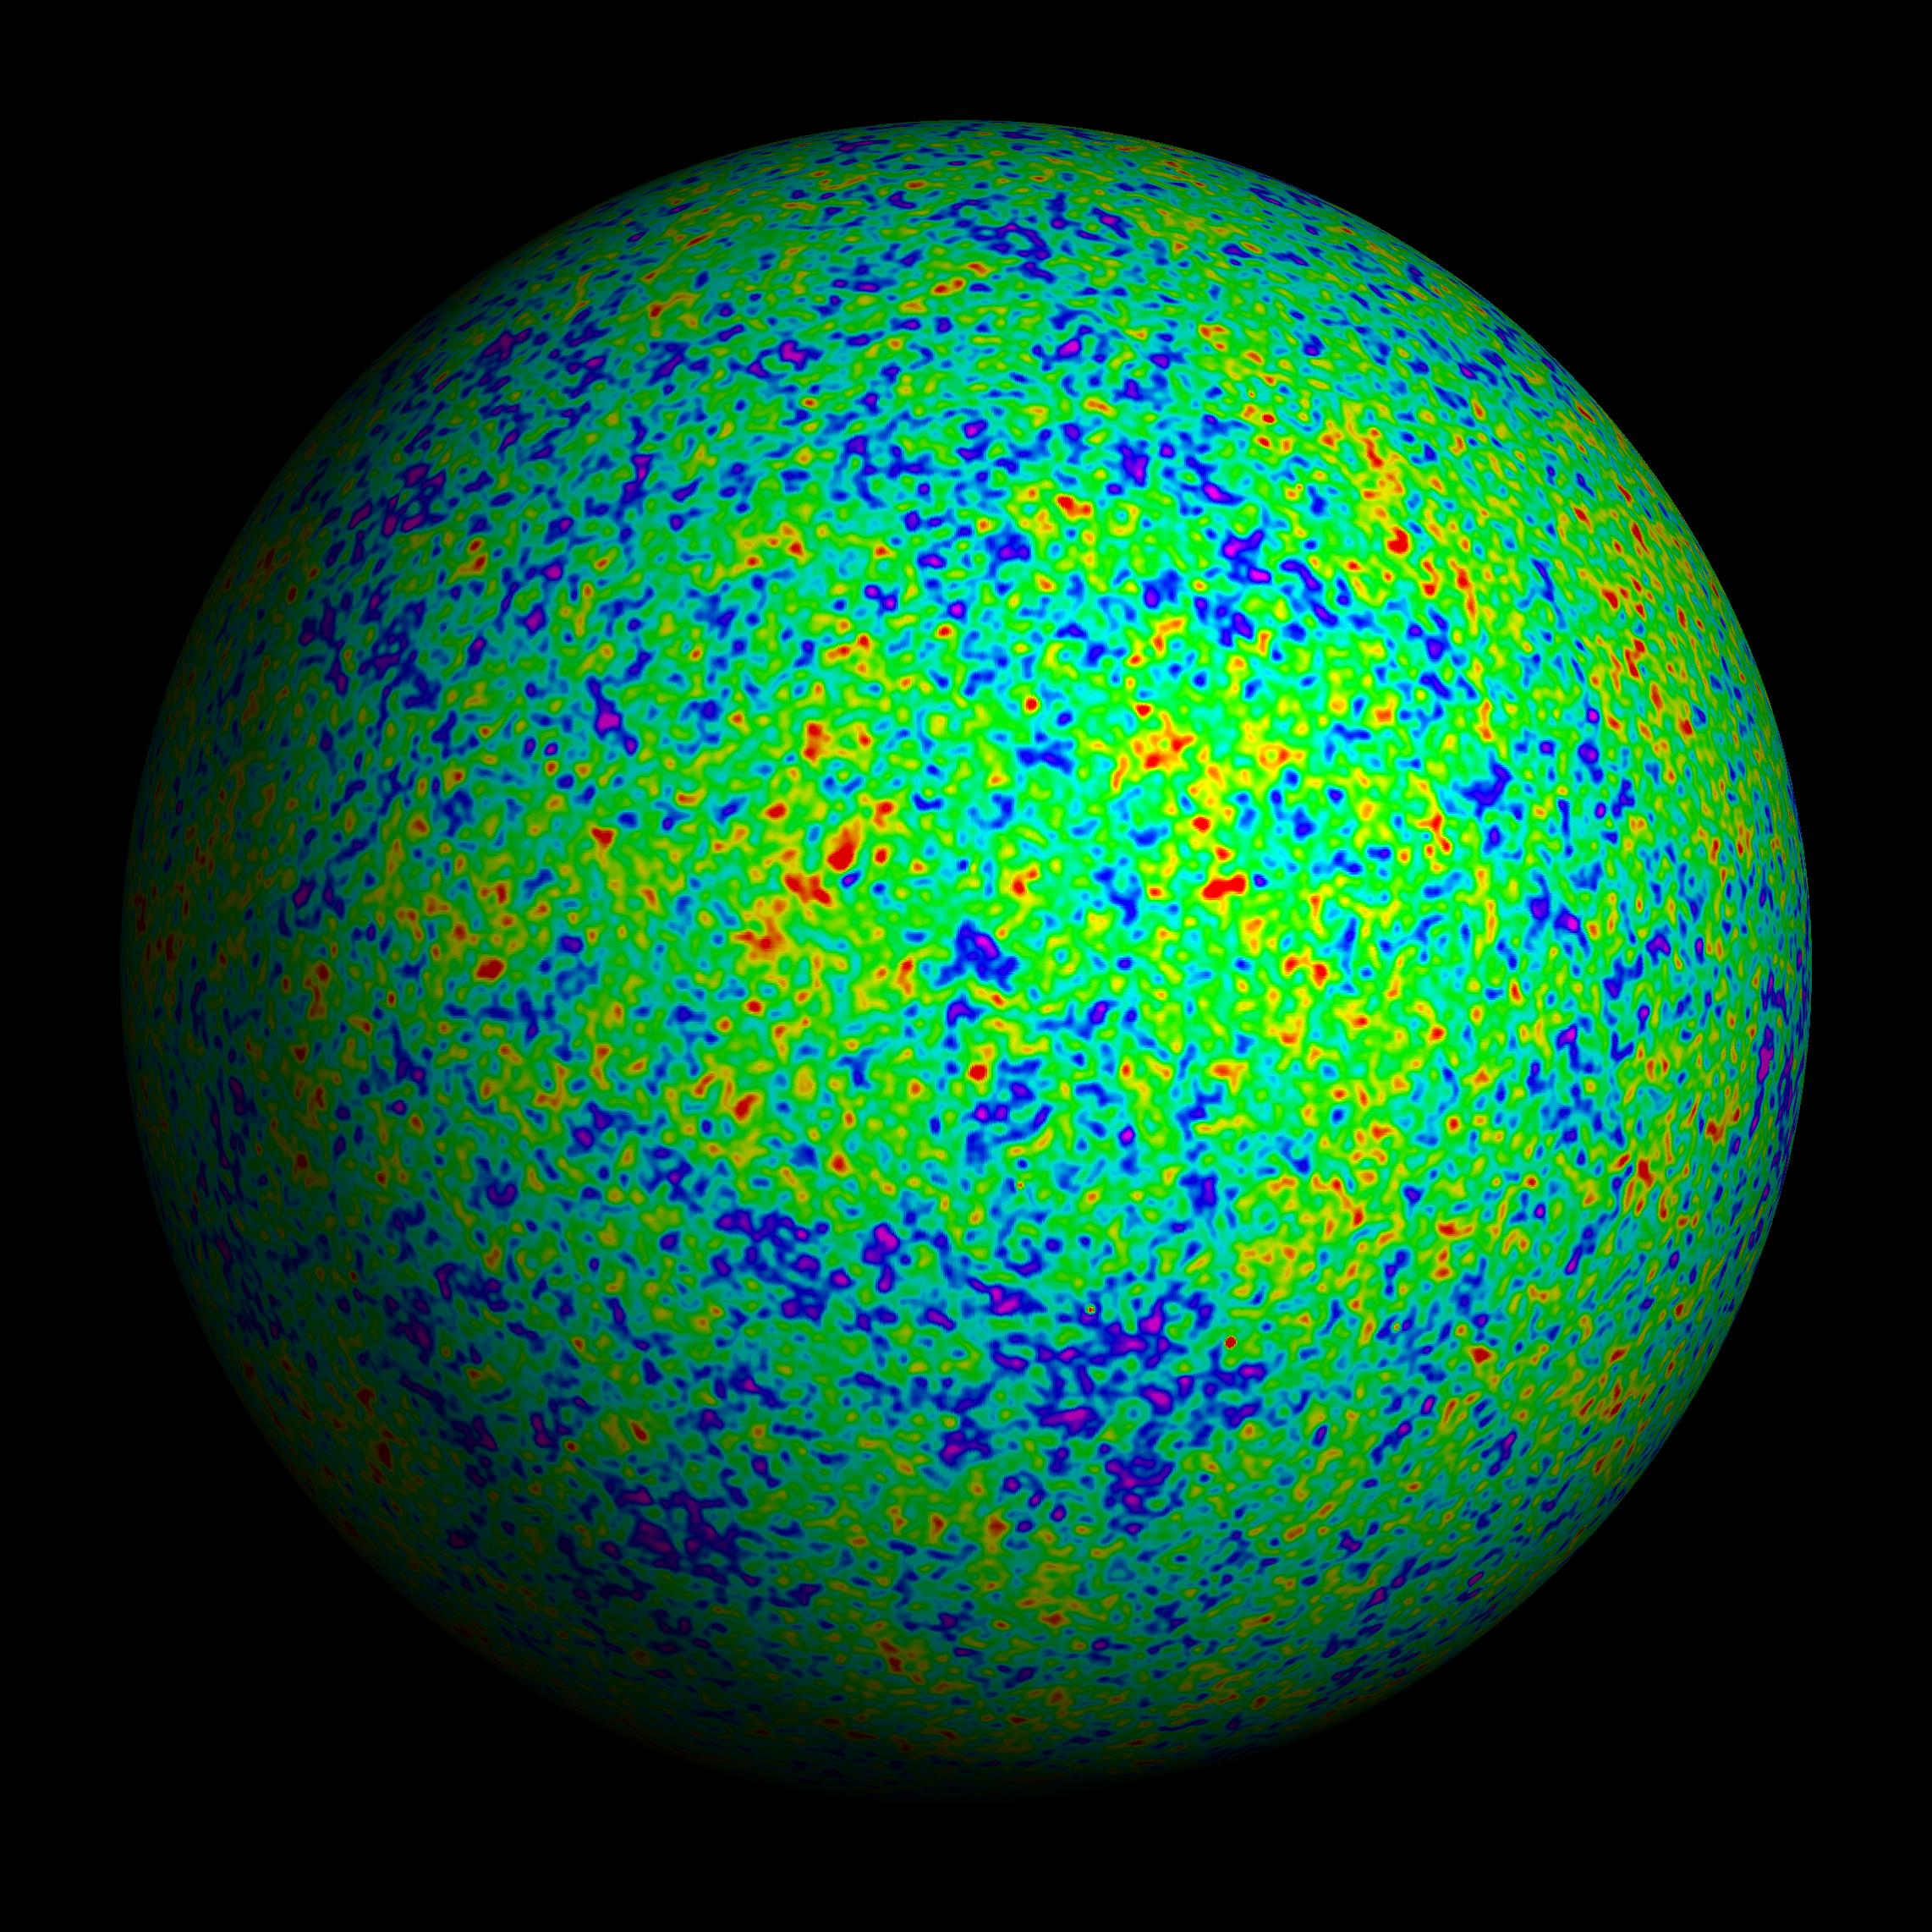
\includegraphics[width=\textwidth]{wiener3yr_map_2284x2284.jpg}
            \end{center}
        \end{column}
    \end{columns}


}


\frame
{
    \begin{center}
        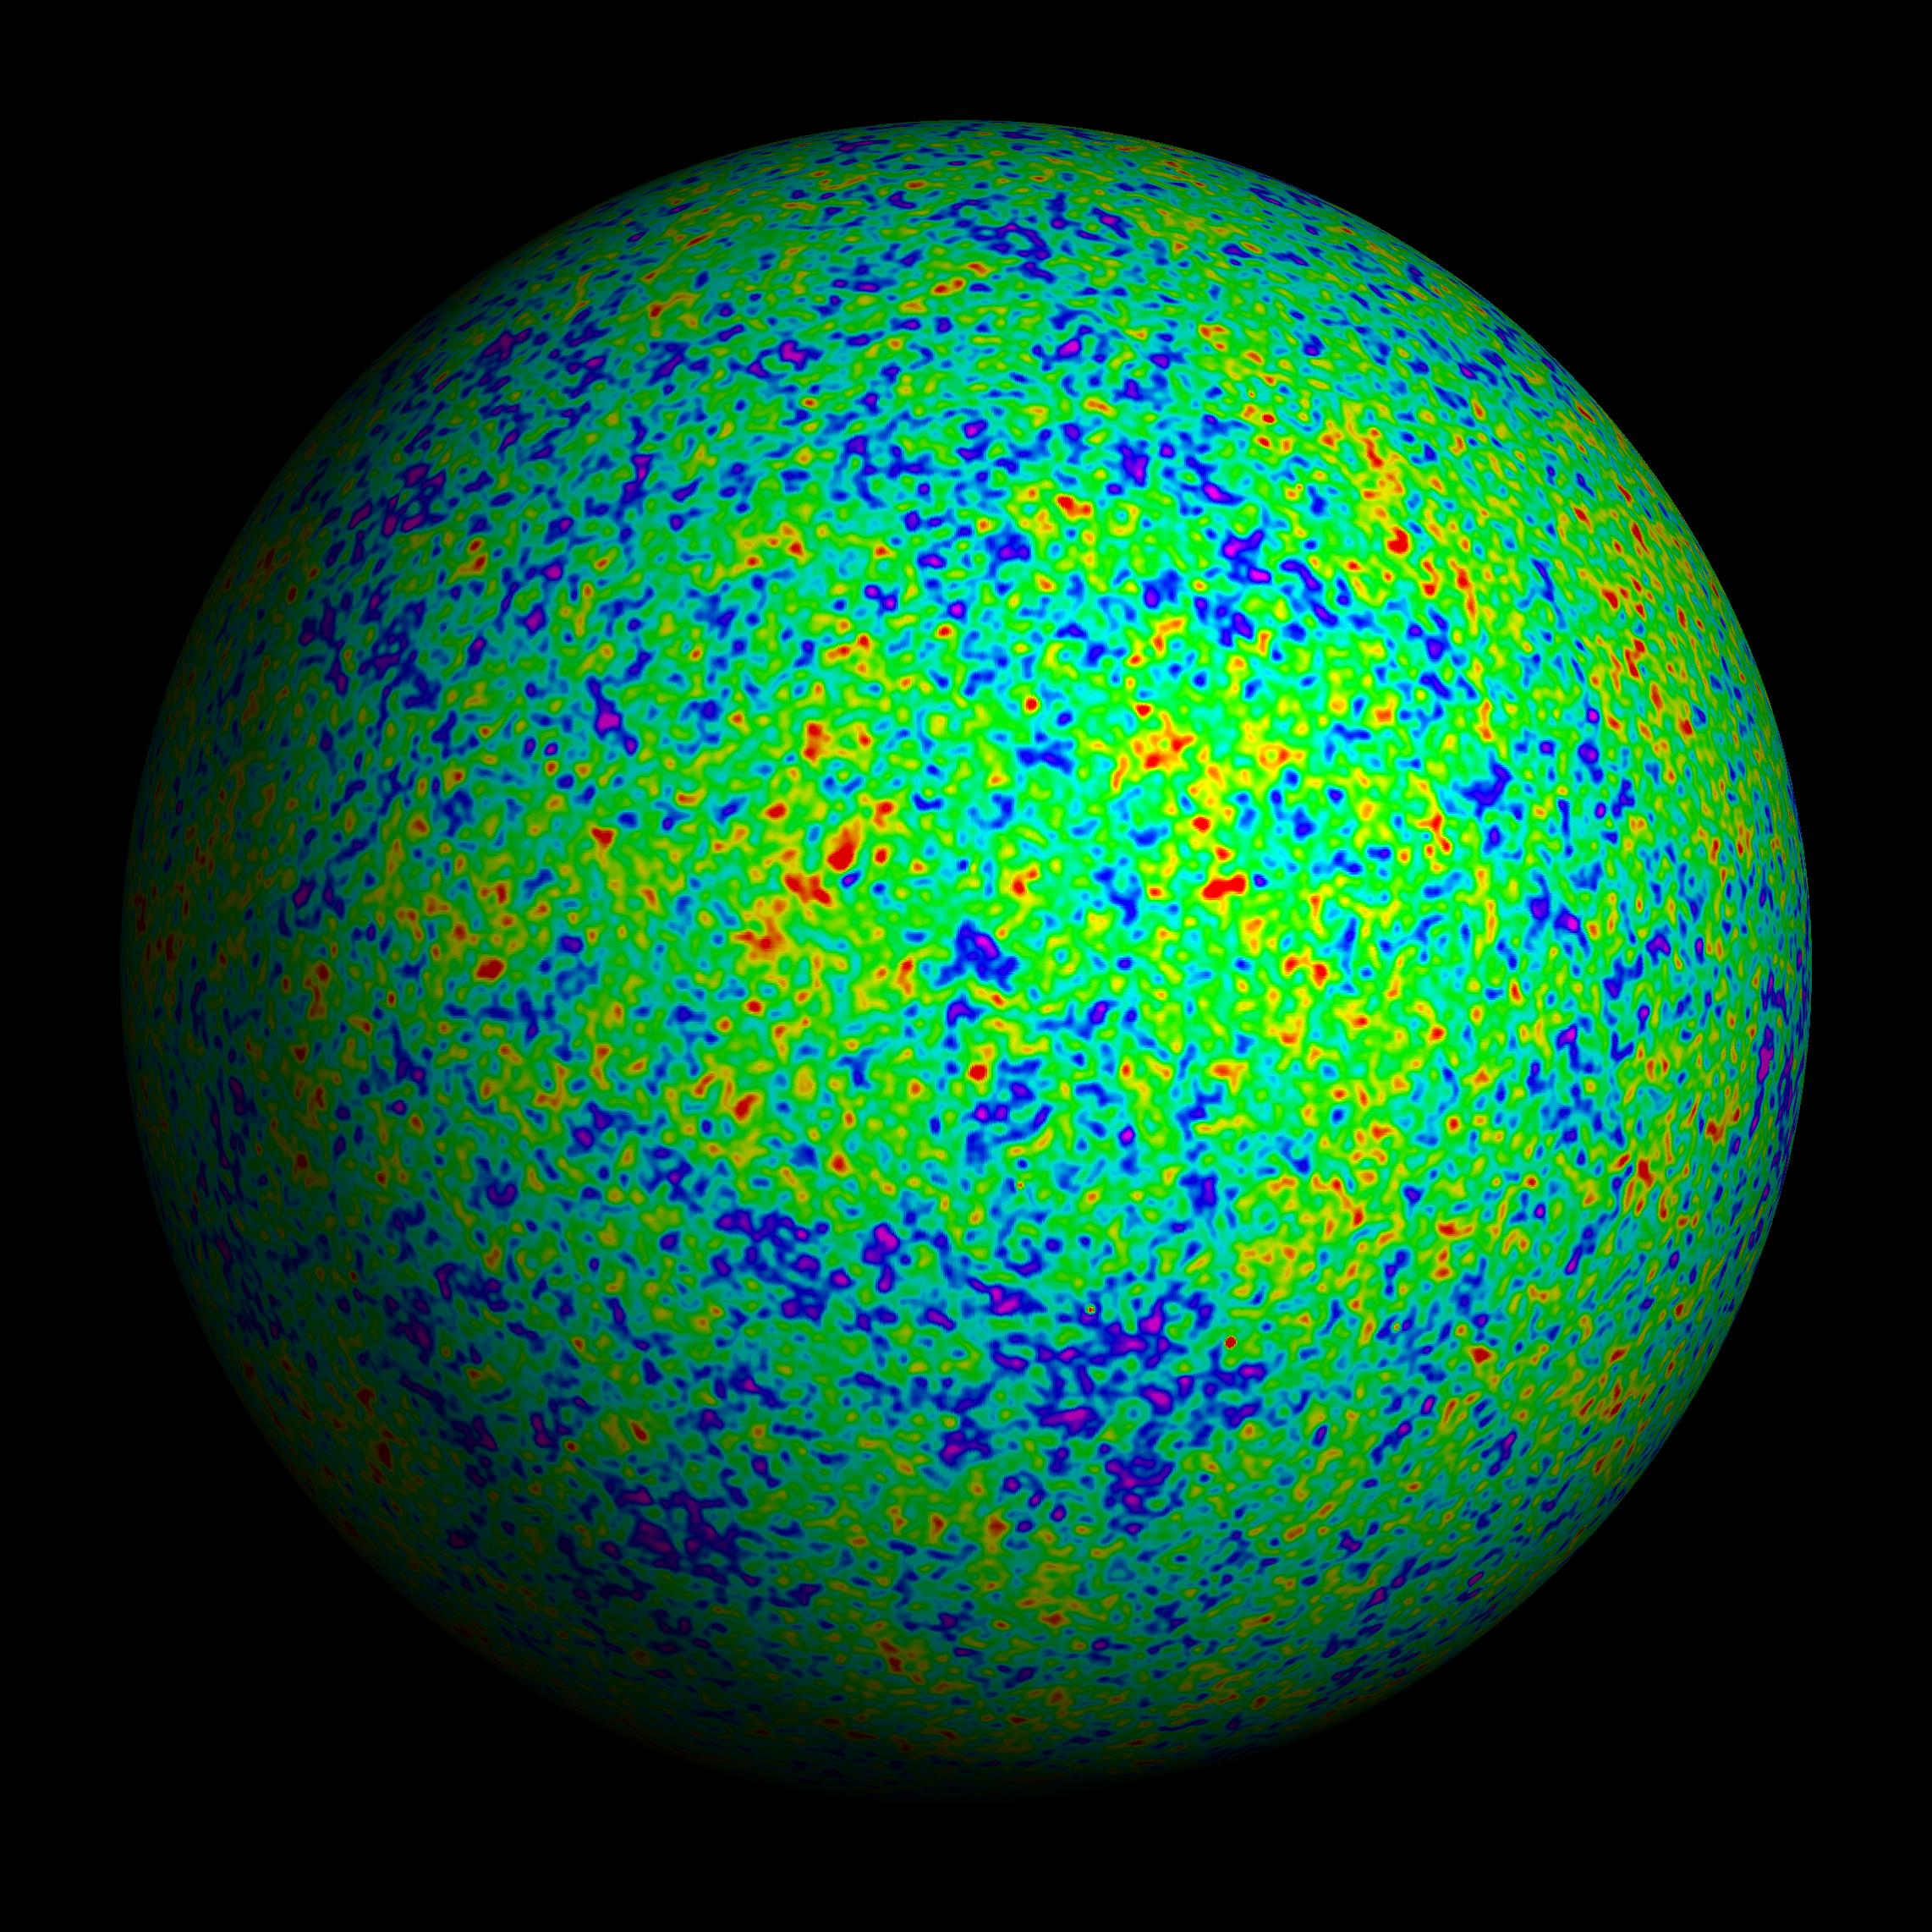
\includegraphics[width=0.75\textwidth]{wiener3yr_map_2284x2284.jpg}
    \end{center}
    {\normalsize Image of the universe 300,000 years after the big bang (Tegmark, WMAP)}
}

\frame
{

    {\huge Optical Astronomy}

}
\frame
{

    \frametitle{Optical Astronomy}

    \setbeamerfont*{itemize/enumerate body}{size=\small}

    \begin{columns}
        \begin{column}{0.5\textwidth}
            \begin{itemize}

                \item It all starts with taking pretty pictures

                \item Optical means visible light, but we also use near infrared
                    and ultraviolet.

            \end{itemize}
        \end{column}
        \begin{column}{0.5\textwidth}
            \begin{center}
                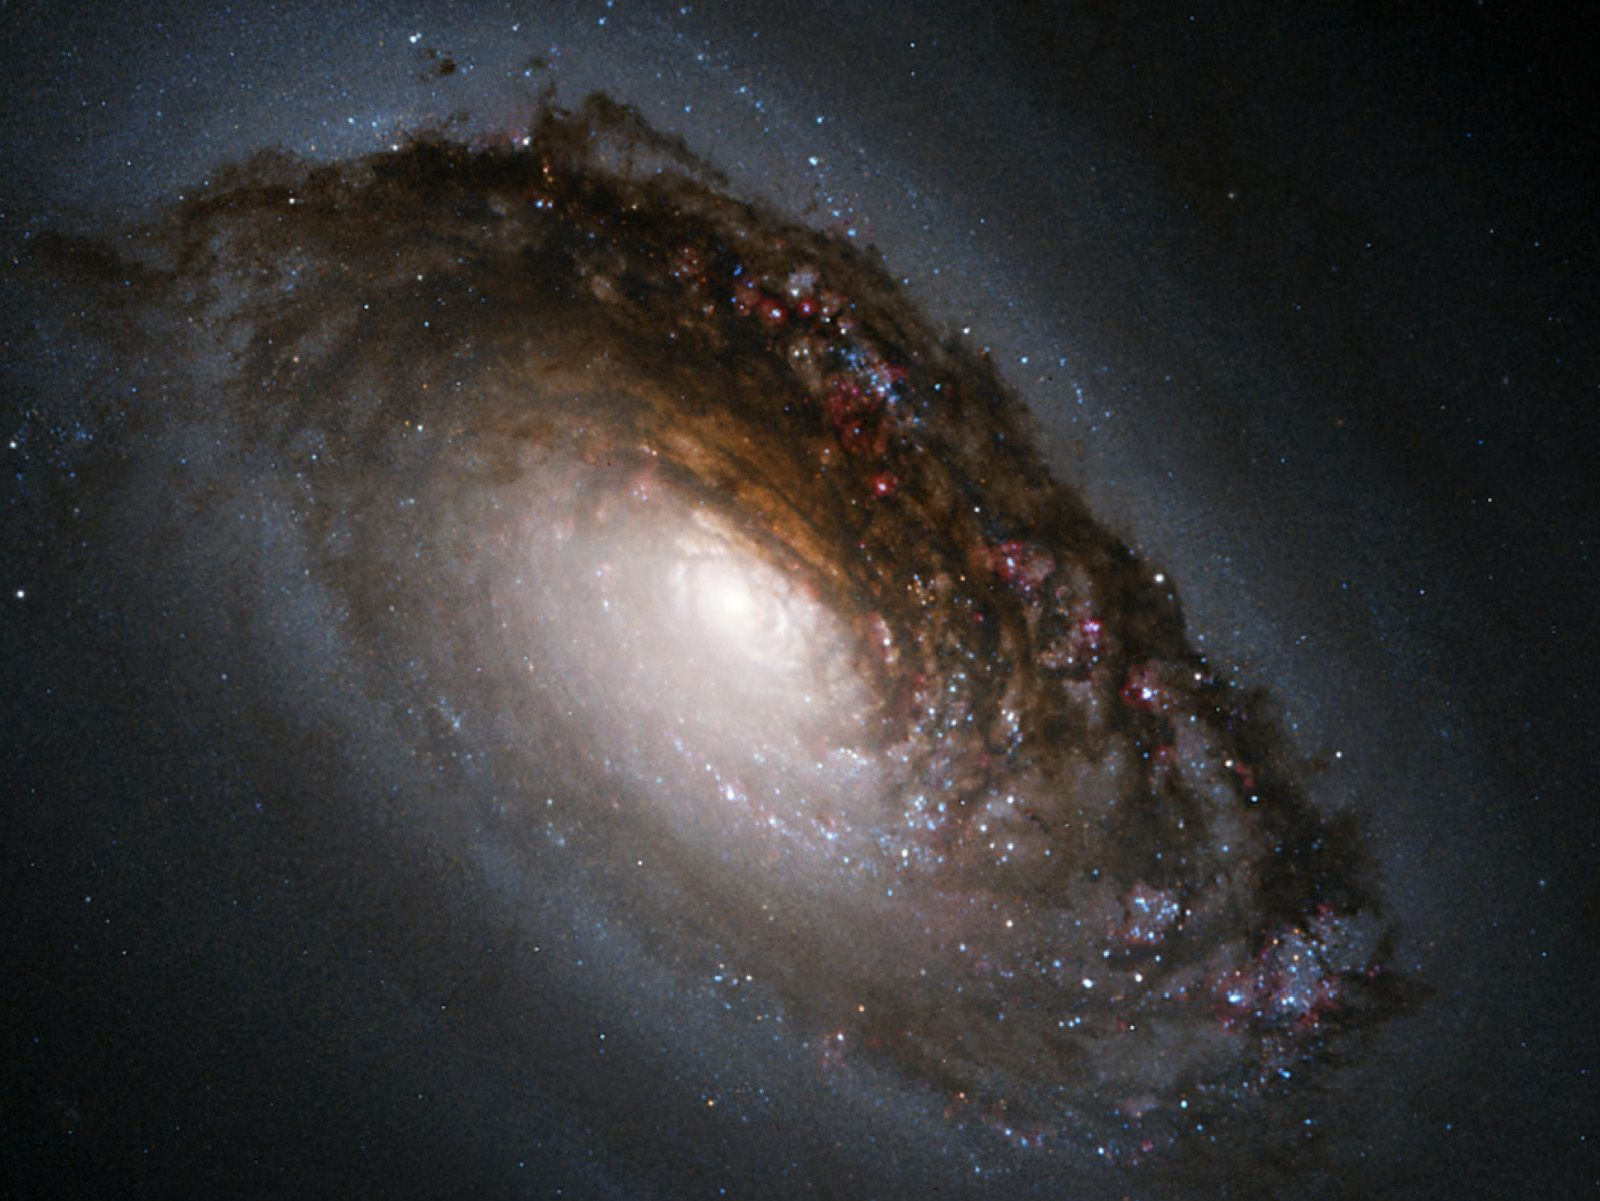
\includegraphics[width=\textwidth]{m64-black-eye-galaxy.jpg}
                \newline
                {\tiny NASA, S. Smartt, D. Richstone}
            \end{center}

            
        \end{column}
    \end{columns}


}

\frame
{

    \frametitle{Optical Astronomy}

    \setbeamerfont*{itemize/enumerate body}{size=\small}

    \begin{columns}
        \begin{column}{0.5\textwidth}
            \begin{itemize}

                \item The primary detectors in astronomical cameras are CCDs,
                    similar to the device in your phone.
                    
                \item The raw data is an array of pixel values



            \end{itemize}
        \end{column}
        \begin{column}{0.5\textwidth}
            \begin{center}
                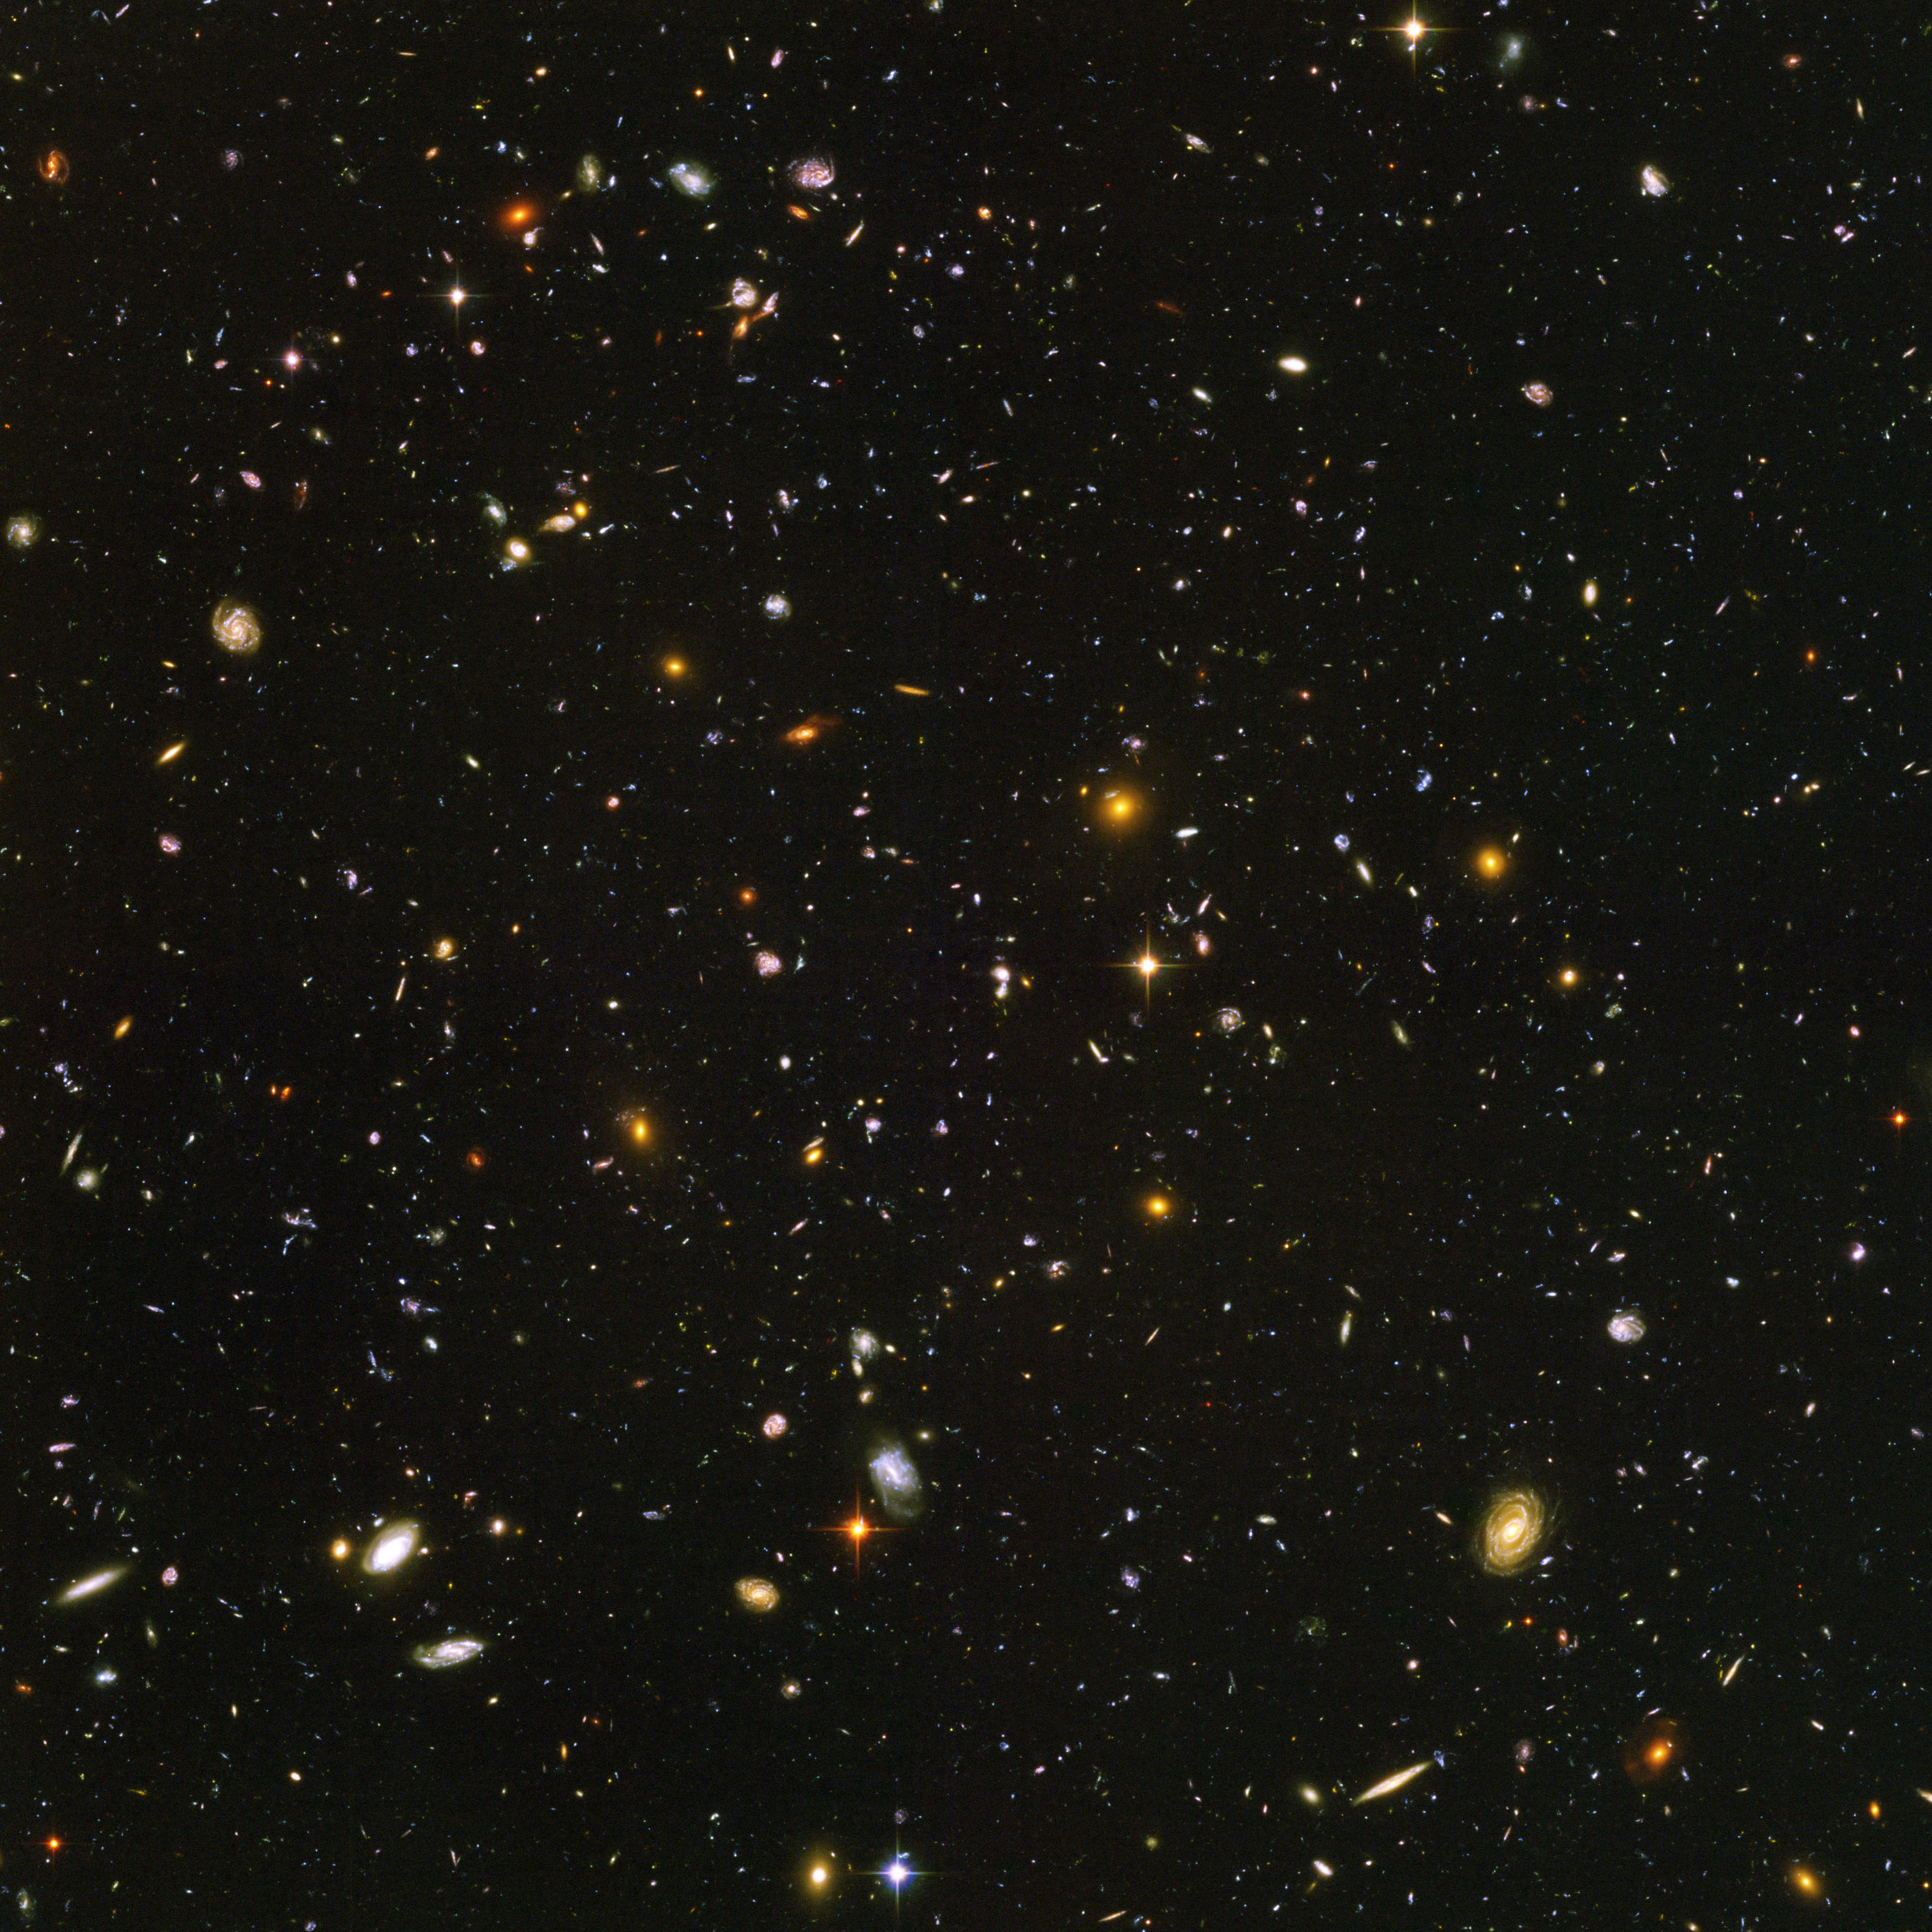
\includegraphics[width=\textwidth]{UDF_half.jpg}
                \newline
                {\tiny Hubble UDF}
            \end{center}

            
        \end{column}
    \end{columns}


}

\frame
{

    \frametitle{Optical Astronomy}

    \setbeamerfont*{itemize/enumerate body}{size=\small}

    \begin{columns}
        \begin{column}{0.5\textwidth}
            \begin{itemize}


                \item The color comes from combining images taken though red,
                    green, and blue filters

                \item Dark Energy Survey sky viewer demo

            \end{itemize}
        \end{column}
        \begin{column}{0.5\textwidth}
            \begin{center}
                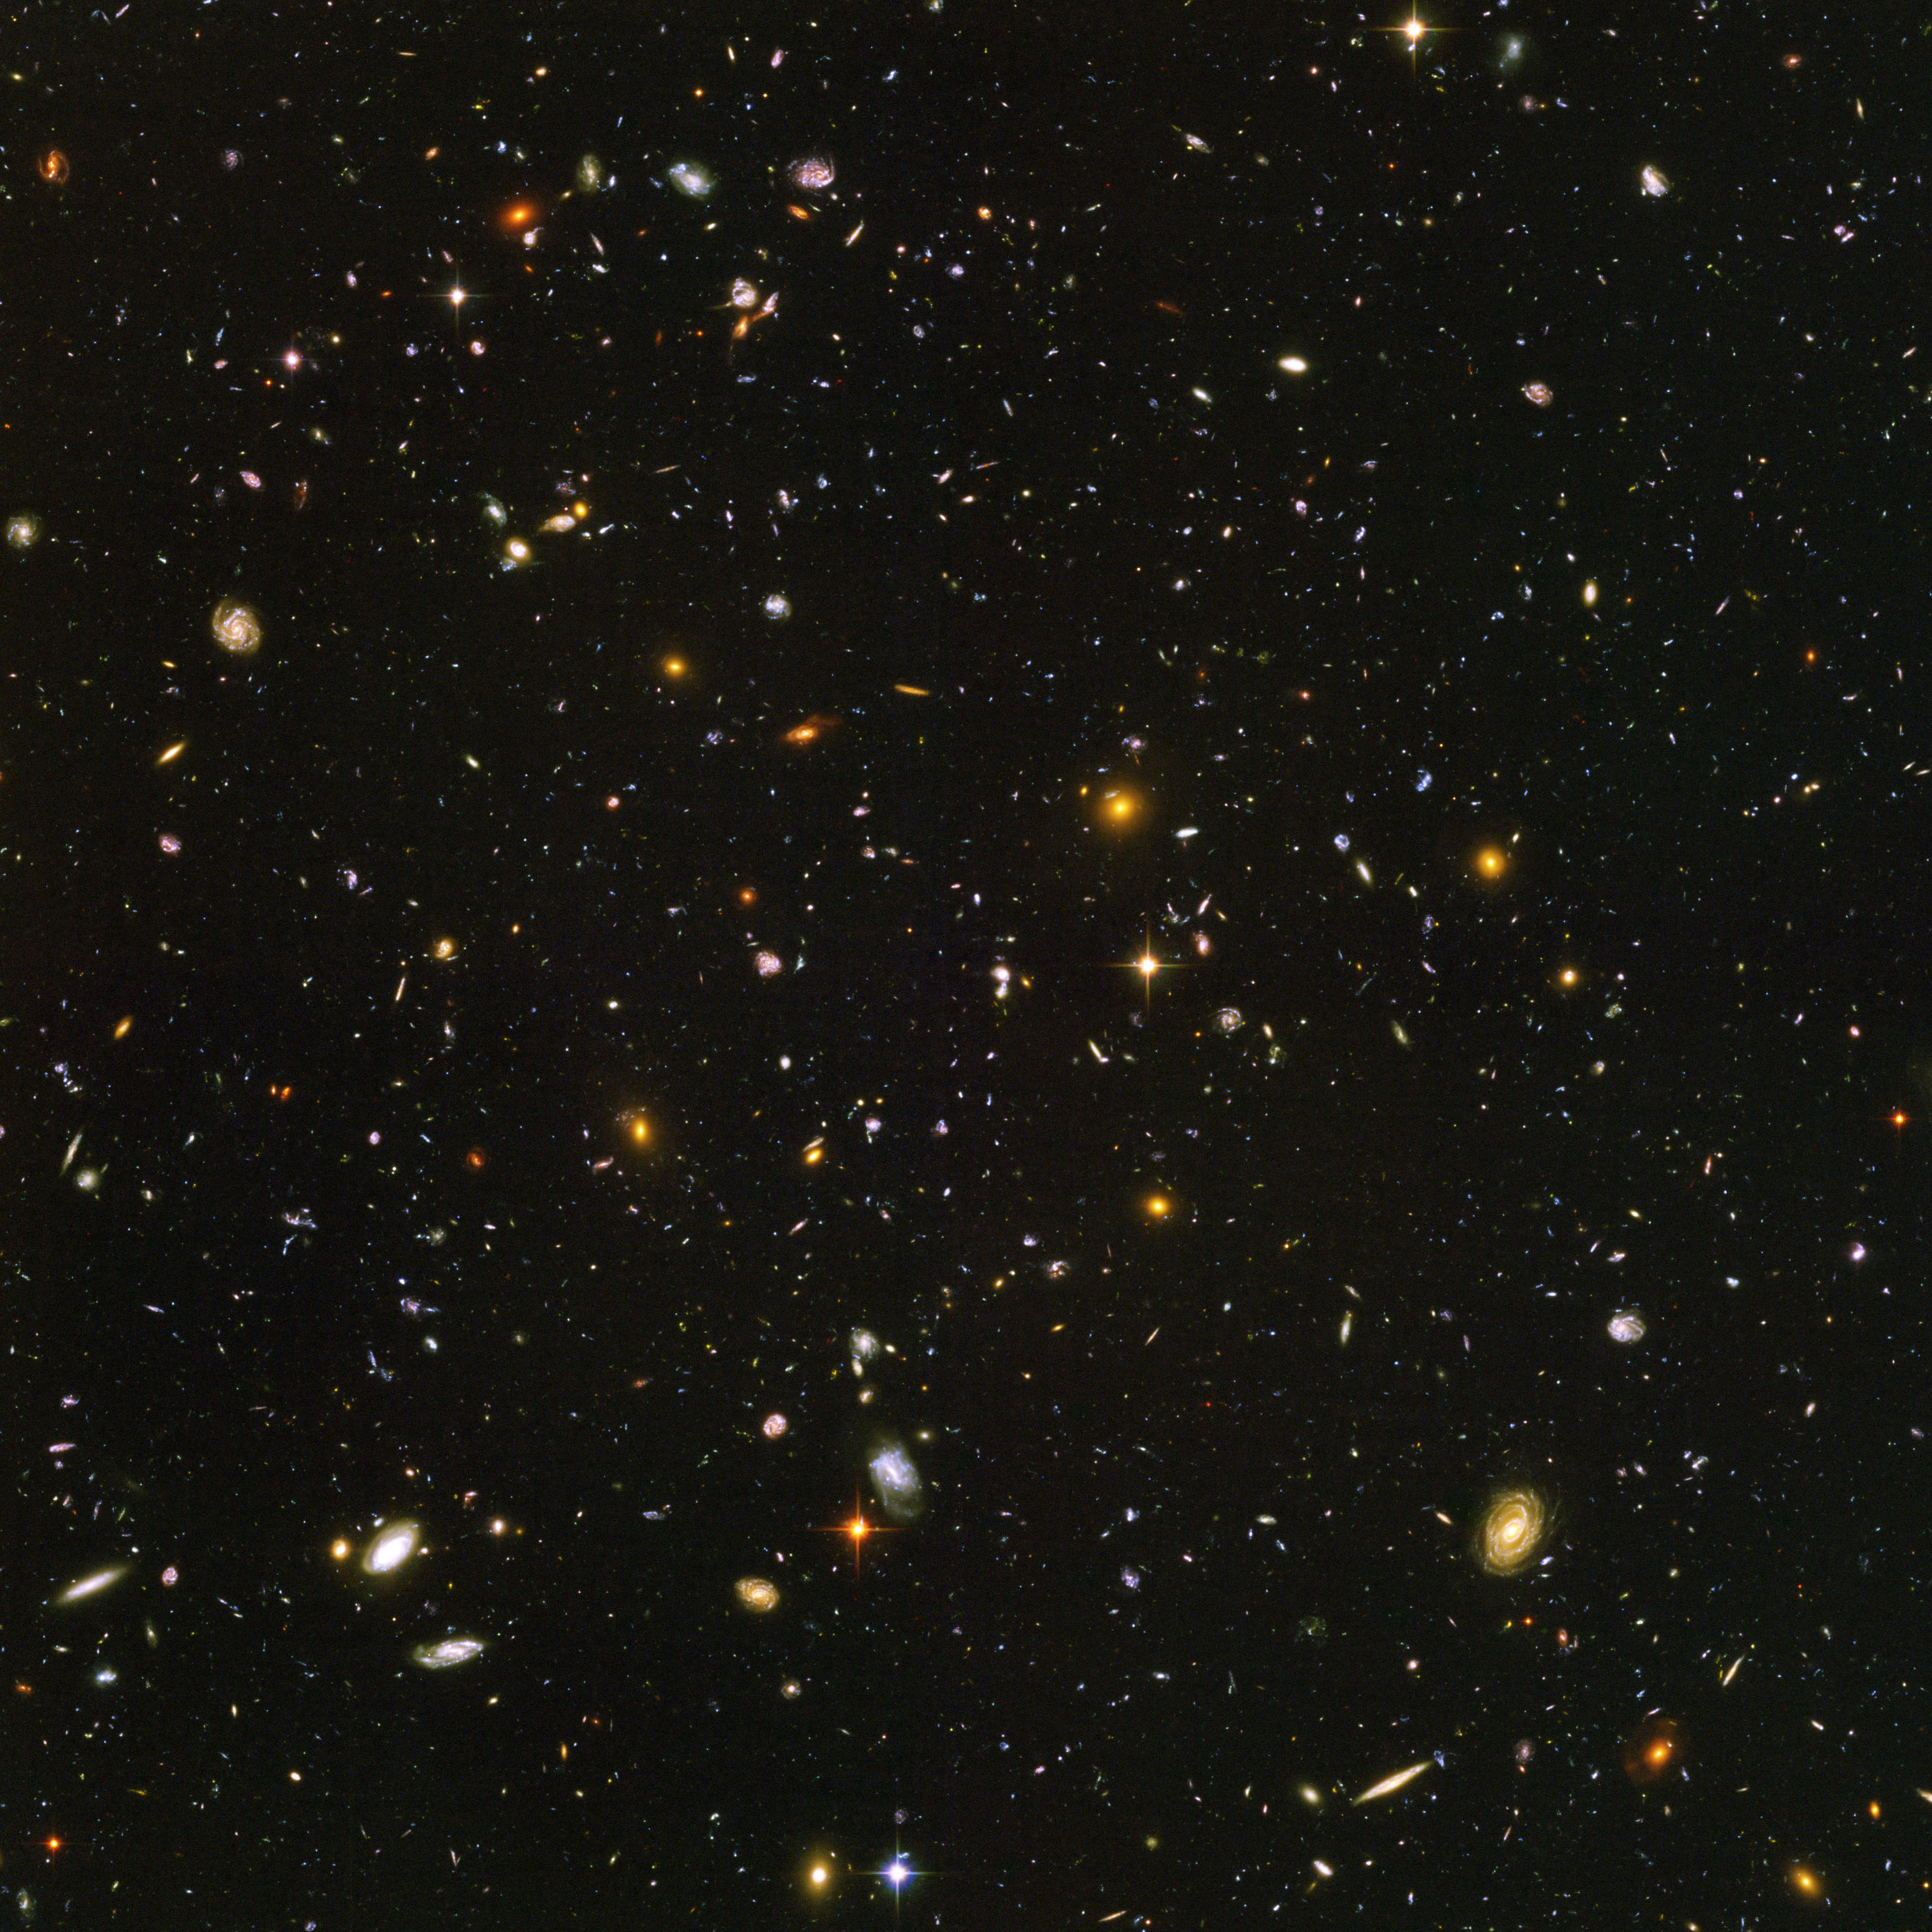
\includegraphics[width=\textwidth]{UDF_half.jpg}
                \newline
                {\tiny Hubble UDF}
            \end{center}

            
        \end{column}
    \end{columns}


}

\frame
{

    \frametitle{Optical Astronomy}

    \setbeamerfont*{itemize/enumerate body}{size=\small}

    \begin{columns}
        \begin{column}{0.5\textwidth}
            \begin{itemize}


                \item We use software to identify objects in the images

                \item We then measure properties of each object, for example

                    \begin{itemize}
                        \item Location
                        \item Brightness
                        \item Size
                        \item Ellipticity
                    \end{itemize}

            \end{itemize}
        \end{column}
        \begin{column}{0.5\textwidth}
            \begin{center}
                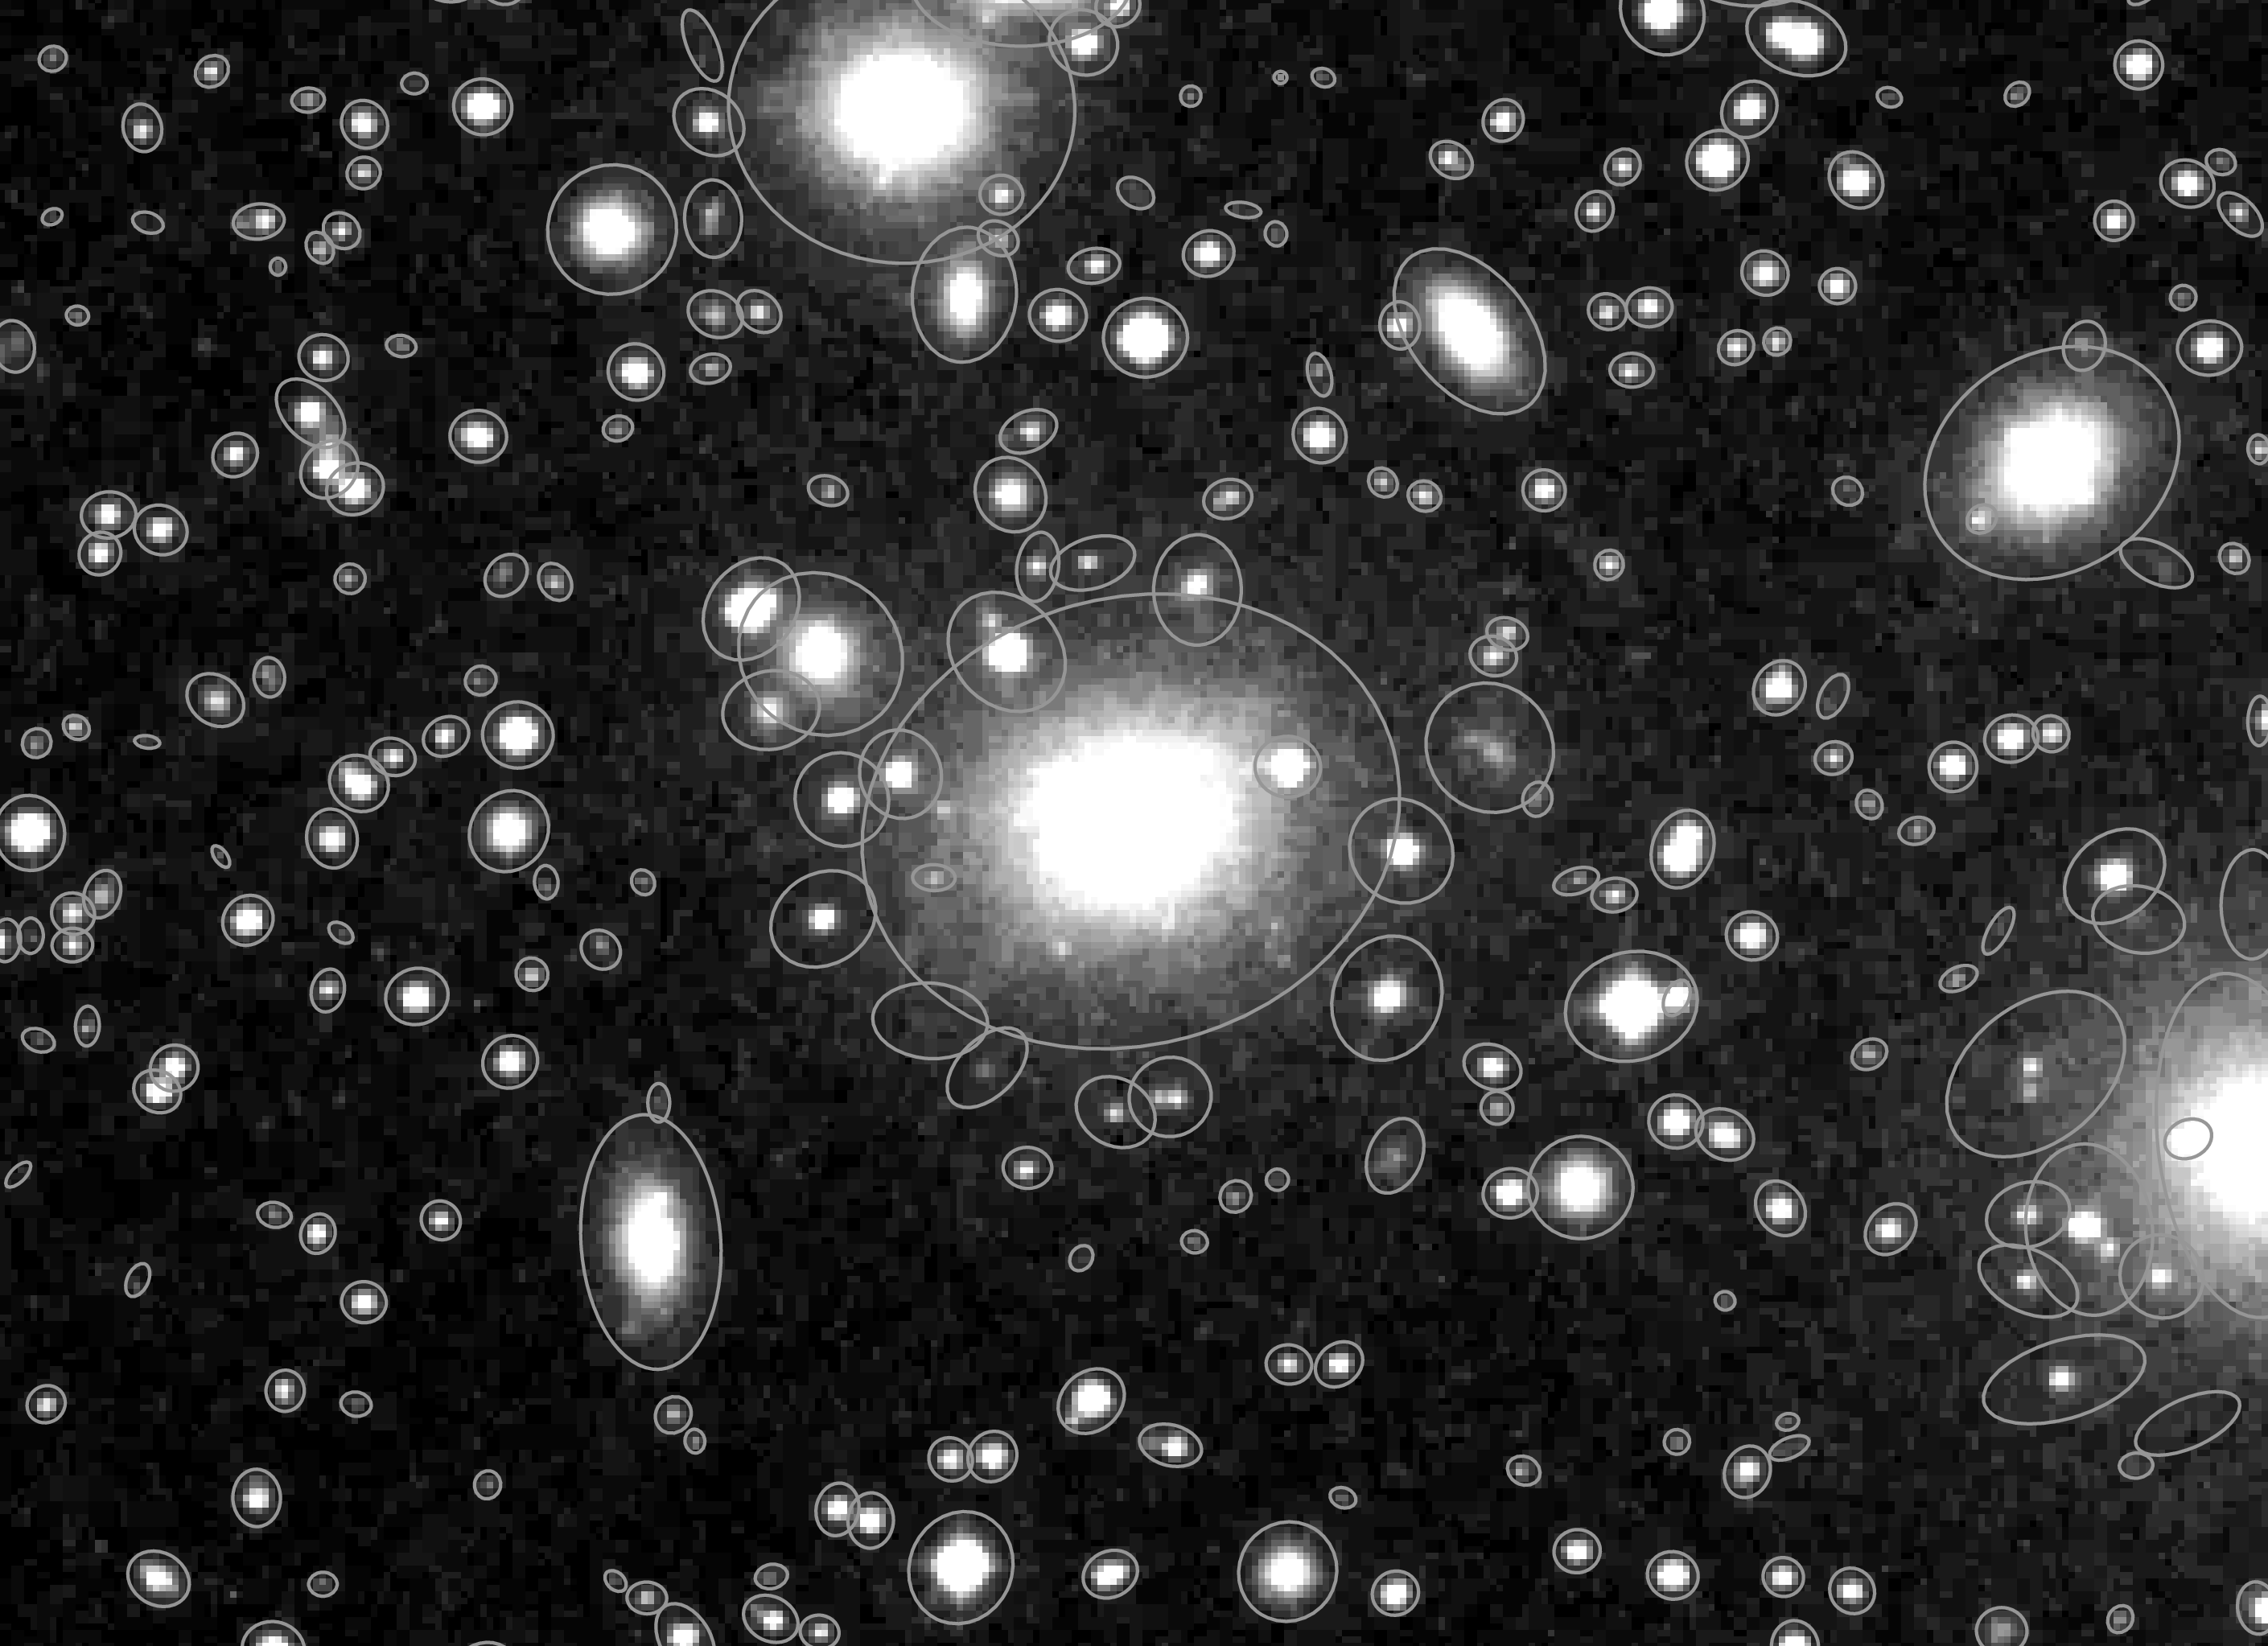
\includegraphics[width=\textwidth]{sun226_fig.png}
                \newline
                {\tiny Source Extractor (Bertin)}
            \end{center}

            
        \end{column}
    \end{columns}


}

\frame
{

    \frametitle{Optical Astronomy}

    \setbeamerfont*{itemize/enumerate body}{size=\small}

    \begin{columns}
        \begin{column}{0.5\textwidth}
            \begin{itemize}

                \item Once we find objects, we can do additional observations

                \item One of the most interesting is to get a spectrum, also
                    usually in the optical/near infrared

                \item Can learn about the chemical composition of the object

                \item For galaxies, can also get the redshift and thus
                    a measure of {\em distance}

            \end{itemize}
        \end{column}
        \begin{column}{0.5\textwidth}
            \begin{center}
                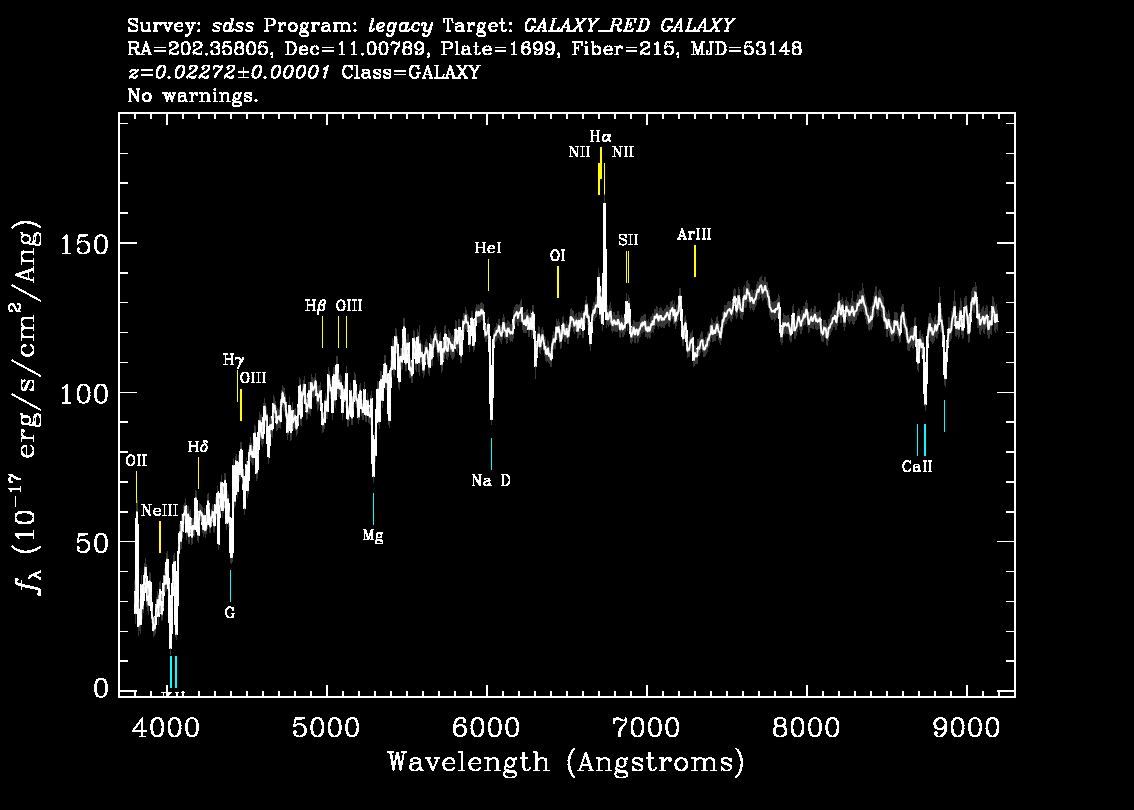
\includegraphics[width=\textwidth]{specById-inv.png}
                \newline
                {\tiny Galaxy spectrum (SDSS)}
            \end{center}

            
        \end{column}
    \end{columns}


}

\frame
{

    \frametitle{Optical Astronomy}

    \setbeamerfont*{itemize/enumerate body}{size=\small}

    \begin{columns}
        \begin{column}{0.5\textwidth}
            \begin{itemize}

                \item It is too time consuming to measure a full spectrunm
                    for every object

                \item We instead estimate redshifts statistically based on
                    measurements through different colored filters

                \item This is a {\em statistical} measure of distance

            \end{itemize}
        \end{column}
        \begin{column}{0.5\textwidth}
            \begin{center}
                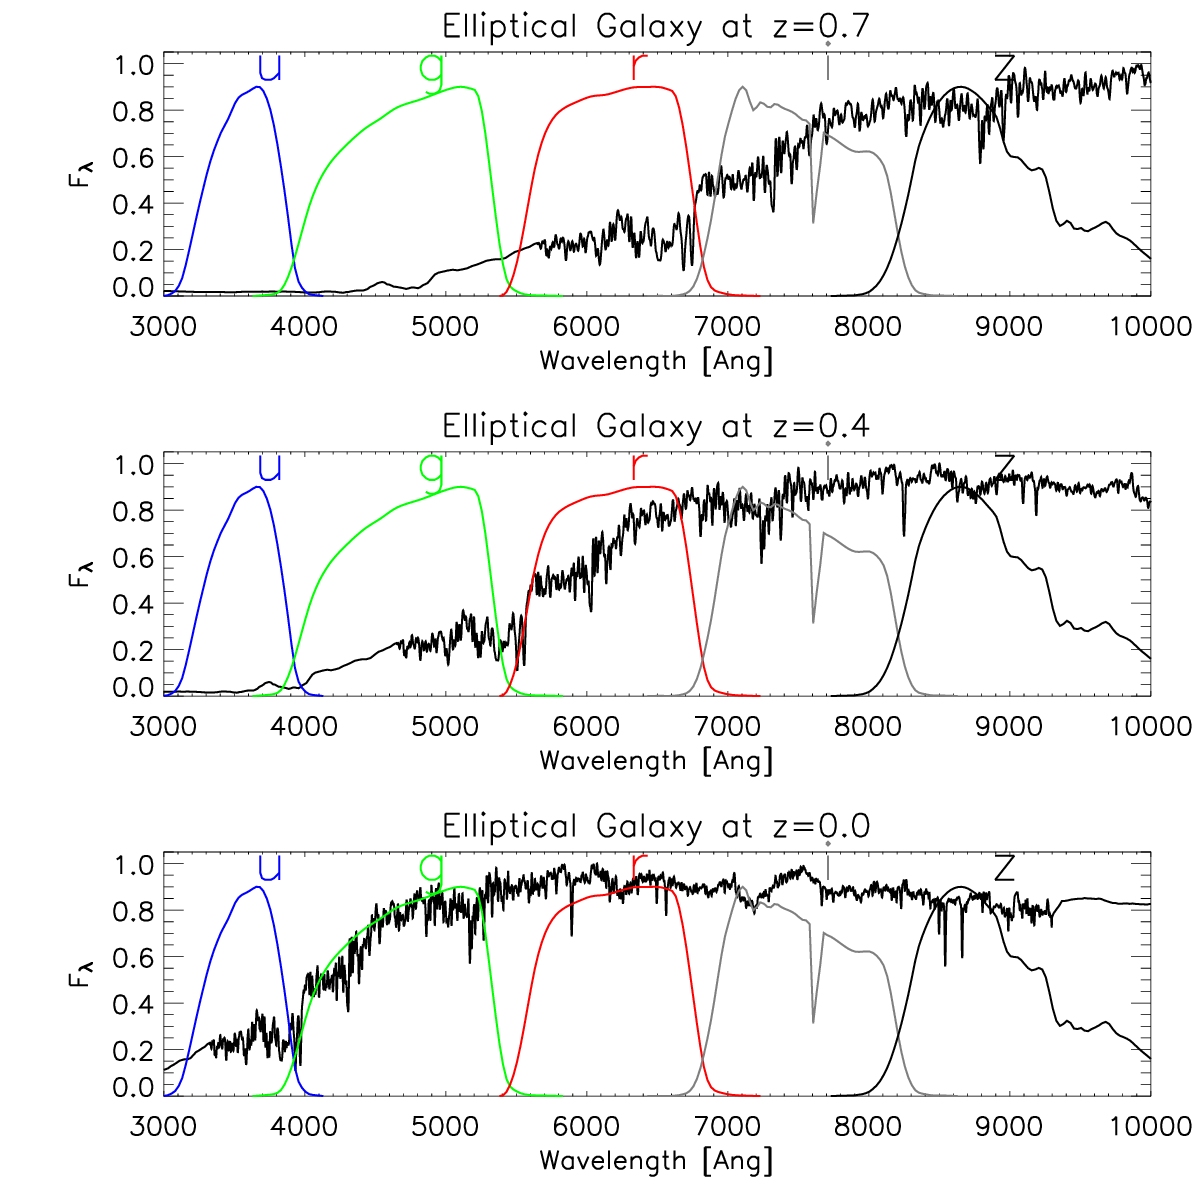
\includegraphics[width=\textwidth]{lrg_spectrum.png}
g               \newline
                {\tiny Galaxy photometric redshift (Padmanabhan)}
            \end{center}

            
        \end{column}
    \end{columns}


}

\frame
{

    \frametitle{Optical Astronomy}


    \begin{itemize}

        \item Thus we have a some basic measurements from optical data.  For
            each object we can measure (among other things)

            \begin{enumerate}

                \item Location on the sky

                \item Distance (velocity/redshift)

                \item Brightness

                \item Color

                \item Size

                \item Ellipticity

            \end{enumerate}


    \end{itemize}

}

\frame
{

    {\huge Cosmology with Optical Astronomy}

}


\frame
{

    \frametitle{Cosmology with Optical Astronomy}


    \begin{itemize}

        \item How can we learn about cosmology from these measurements?

        \item First let's discuss what the theory can predict.

    \end{itemize}

}

\frame
{

    \frametitle{What Theory Predicts}

    \setbeamerfont*{itemize/enumerate body}{size=\large}

    \begin{itemize}

        \item The theory is gravity (general relativity) with dark matter, dark
            energy, and normal matter.

        \item The theory can predict (among other things):
            
            \begin{itemize}

                \item How the universe expands over time.

                \item How the light from distant galaxies is redshifted

                \item How the matter within the universe reacts to gravity, known
                    as ``clustering''.

            \end{itemize}

    \end{itemize}

}


\frame
{

    \frametitle{What Theory Predicts}


    \setbeamerfont*{itemize/enumerate body}{size=\large}

    \begin{itemize}

        \item How the universe is expanding

            \begin{itemize}
                    
                \item For two given galaxies, the distance between changes over
                    time {\color{gold} $|\Delta \vec{r} (t)|$ =
                     $| \vec{r}_1 - \vec{r}_2 |(t) $ }

                \item The relative velocity between galaxies is larger
                    for more separated galaxies

            \end{itemize}

        \item How the light from distant galaxies is redshifted {\color{gold}
            $z(|\Delta \vec{r}|)$}

        \item How the matter within the universe reacts to gravity over time.
            Gravity pulls matter together, and the density field
            in the universe evolves {\color{gold} $\rho(\vec{r},t)$}



    \end{itemize}

}

\frame
{

    \frametitle{What Theory Predicts}


    \begin{itemize}

            

        \item Expansion history: {\color{gold} $|\Delta \vec{r} (t)|$ }


        \item Redshift: {\color{gold} $z(|\Delta \vec{r}|)$}


        \item Density evolution: {\color{gold} $\rho(\vec{r},t)$}


        \item Using these measurements we can learn about the mass density in
            the universe (the predictions are actually relative to mean)
            
        \item We can learn about the properties of dark energy



    \end{itemize}

}

\frame
{

    \frametitle{Distance, Redshift and Density}

    \setbeamerfont*{itemize/enumerate body}{size=\large}

    \begin{itemize}

        \item The theory doesn't predict our particular universe

        \item The theory predicts {\em statistics} about these quantities
            
        \item Given the mean and variance of the mass density field, and the
            density of dark energy, it can predict

            \begin{itemize}

                \item {\color{gold} $\langle |\Delta \vec{r} (t)| \rangle$ }: Averaged
                    over a large number of objects

                \item {\color{gold} $\langle z(|\Delta \vec{r}|) \rangle$}

                \item {\color{gold} $\langle \rho(\vec{r_1}) \rho(\vec{r_2})
                    \rangle$ }: Correlation function

            \end{itemize}

    \end{itemize}

}

\frame
{

    \frametitle{Cosmology with Distance, Redshift and Density}


    \begin{itemize}

        \item I'll give two examples of how we do this in practice


    \end{itemize}

}



\frame
{

    \frametitle{Distances and Redshift}

    \setbeamerfont*{itemize/enumerate body}{size=\large}

    \begin{itemize}

        \item In terms of the expansion, it is the combination of {\color{gold}
            $|\Delta \vec{r} (t)| $ } and {\color{gold} $z(|\Delta \vec{r}|)$}
            that is powerful


        \item Let's call this combination  {\color{gold} $D(z)$}, the relationship
            between the distance and redshift.

        \item Typically one of the points is fixed on us, and the other is
            some distant galaxy. So {\color{gold} $D(z)$} means the distance
            to some galaxy with known redshift $z$.

        \item We can measure $z$ directly on a spectrum.  The key is getting
            the distance.

        \item An easy-to-understand method is the standard candle.

    \end{itemize}

}

\frame
{

    \frametitle{Standard Candles}


    \begin{itemize}

        \item If you know the intrinsic luminosity of an object, then you can
            calculate the distance from the {\em apparent brightness}

        \item {\color{gold} $\ell = \frac{L}{4 \pi d^2}$ }

        \item Type 1A supernovae are such objects.

    \end{itemize}

}

\frame
{

    \frametitle{Type 1A Supernovae}

    \setbeamerfont*{itemize/enumerate body}{size=\large}

    \begin{itemize}

        \item We can thus measure {\color{gold} $D(Z)$} using optical astronomy 

            \begin{enumerate}

                \item Take images of the sky, identify objects, measure their brightness

                \item Take more images, on a regular schedule

                \item Watch for a star to go Supernova in a distant
                    galaxy: they get a lot brighter

                \item Go get a spectrum and determine the redshift.

                \item Infer the distance

                \item Average over lots of these to get {\color{gold} $\langle
                    D(z) \rangle$ }

            \end{enumerate}

    \end{itemize}

}

\frame
{

    \begin{center}
        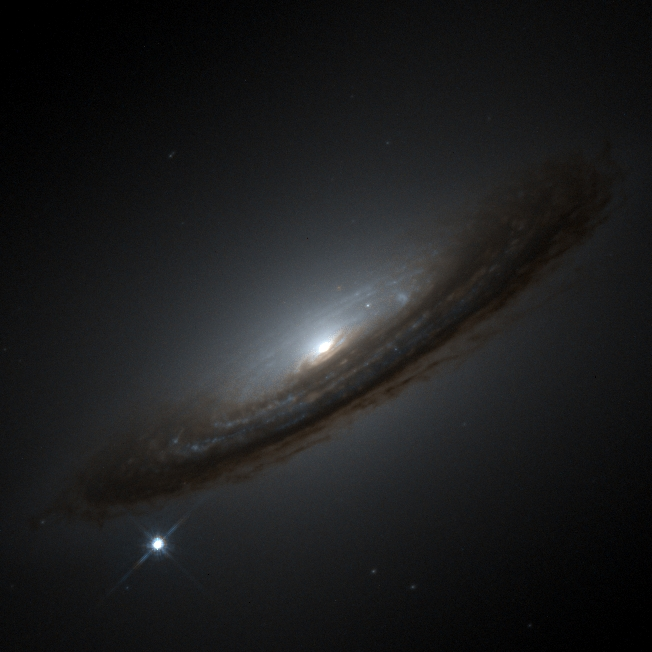
\includegraphics[height=0.9\textheight]{sn94d_hiz_big.jpg}
    \end{center}
    {\normalsize High-Z Supernova Search Team/HST }
}
\frame
{

    \frametitle{Type 1A Supernovae}

    \setbeamerfont*{itemize/enumerate body}{size=\large}

    \begin{columns}
        \begin{column}{0.5\textwidth}
            \begin{itemize}

                \item This is how Dark Energy was discovered 

                \item No predictions with without dark energy are consistent
                    with the measurements

                \item Confirmed by other methods (BAO)

            \end{itemize}

        \end{column}
        \begin{column}{0.5\textwidth}
            \begin{center}
                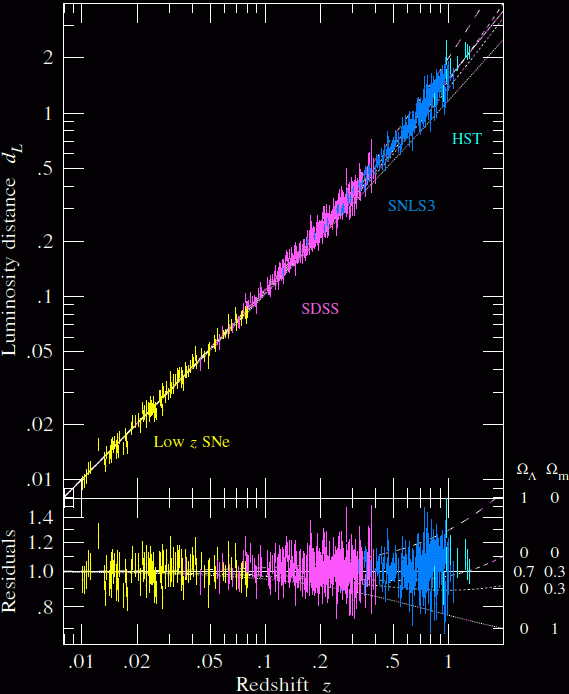
\includegraphics[width=\textwidth]{snhubblediag_betoule_inv.png}
            \end{center}
        \end{column}

    \end{columns}


}

\frame
{

    \frametitle{Correlation Functions}

    \setbeamerfont*{itemize/enumerate body}{size=\small}

    \begin{columns}
        \begin{column}{0.5\textwidth}
            \begin{itemize}

                \item The theory predicts the correlation function of
                    dark matter {\color{gold} $\langle \rho(\vec{r_1}) \rho(\vec{r_2})
                    \rangle$ }

                \item It also predicts how it evolves with time
                    
                \item The amplitude increases over time because gravity pulls
                    matter together, making it more spatially correlated


            \end{itemize}

        \end{column}
        \begin{column}{0.5\textwidth}
            \begin{center}
                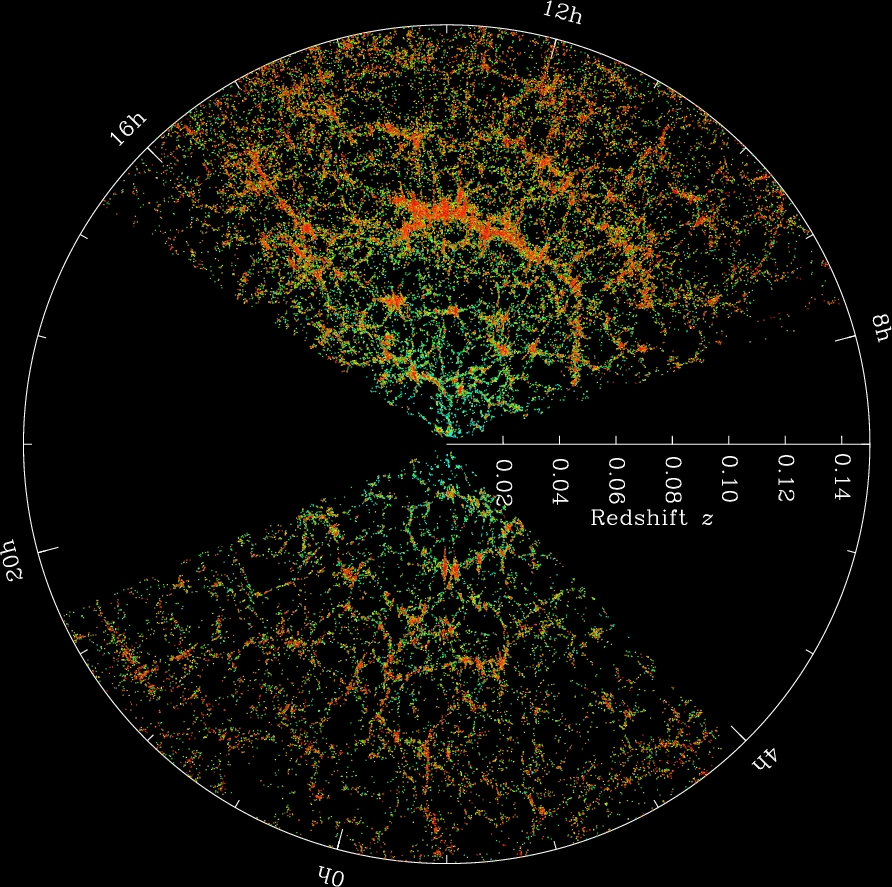
\includegraphics[width=\textwidth]{orangepie.jpg}
            \end{center}
            {\tiny SDSS Galaxy Locations (M. Blanton)}
        \end{column}

    \end{columns}


}

\frame
{

    \frametitle{Dark Matter Correlation Function}

    \setbeamerfont*{itemize/enumerate body}{size=\small}

    \begin{columns}
        \begin{column}{0.5\textwidth}
            \begin{itemize}

                \item The theory predicts the correlation function of
                    dark matter {\color{gold} $\langle \rho(\vec{r_1}) \rho(\vec{r_2})
                    \rangle$ }

                \item Depends on the mean density and variance of the matter 
                    in the universe

                \item Evolution depends on the dark energy
 
                \item We can measure this using
                    {\color{lightskyblue} gravitational lensing}

            \end{itemize}

        \end{column}
        \begin{column}{0.5\textwidth}
            \begin{center}
                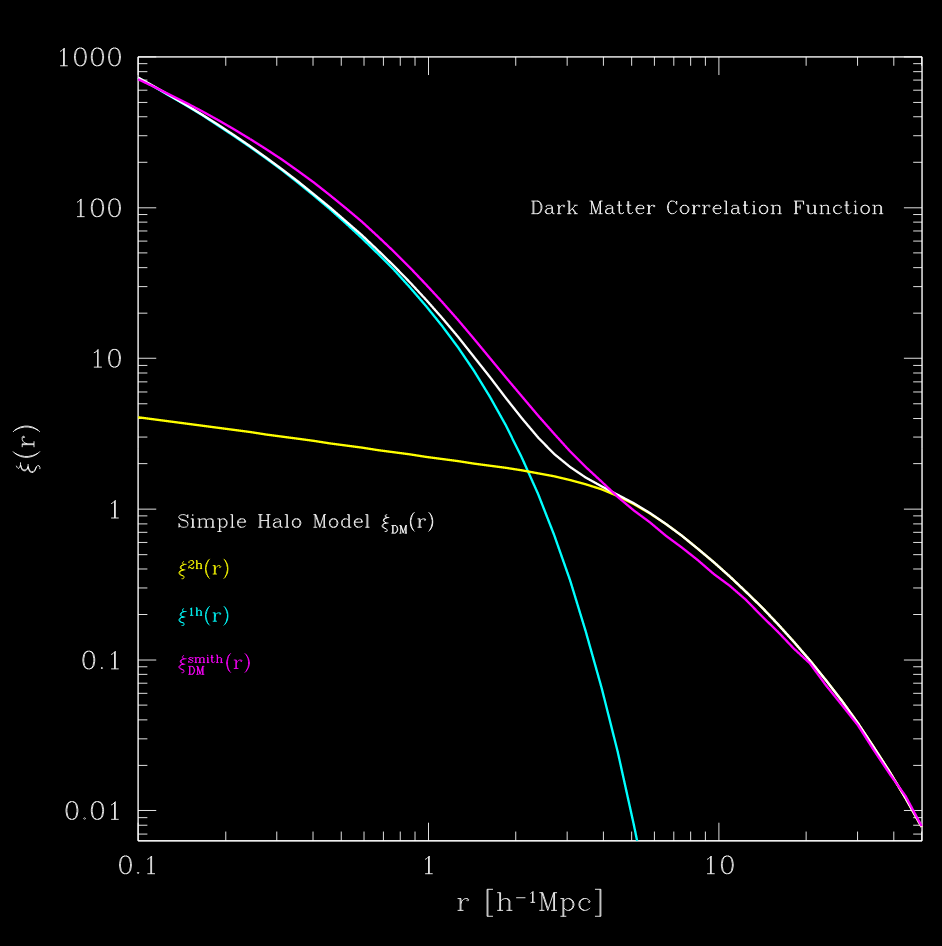
\includegraphics[width=\textwidth]{zentner-halo-model-inv.png}
            \end{center}
            {\tiny A. Zentner}
        \end{column}

    \end{columns}


}


\frame
{
            \begin{center}
                \includegraphics[width=\textwidth]{A_Horseshoe_Einstein_Ring_from_Hubble.JPG}
            \end{center}
            {\tiny HST/NASA}

    
}
\frame
{
            \begin{center}
                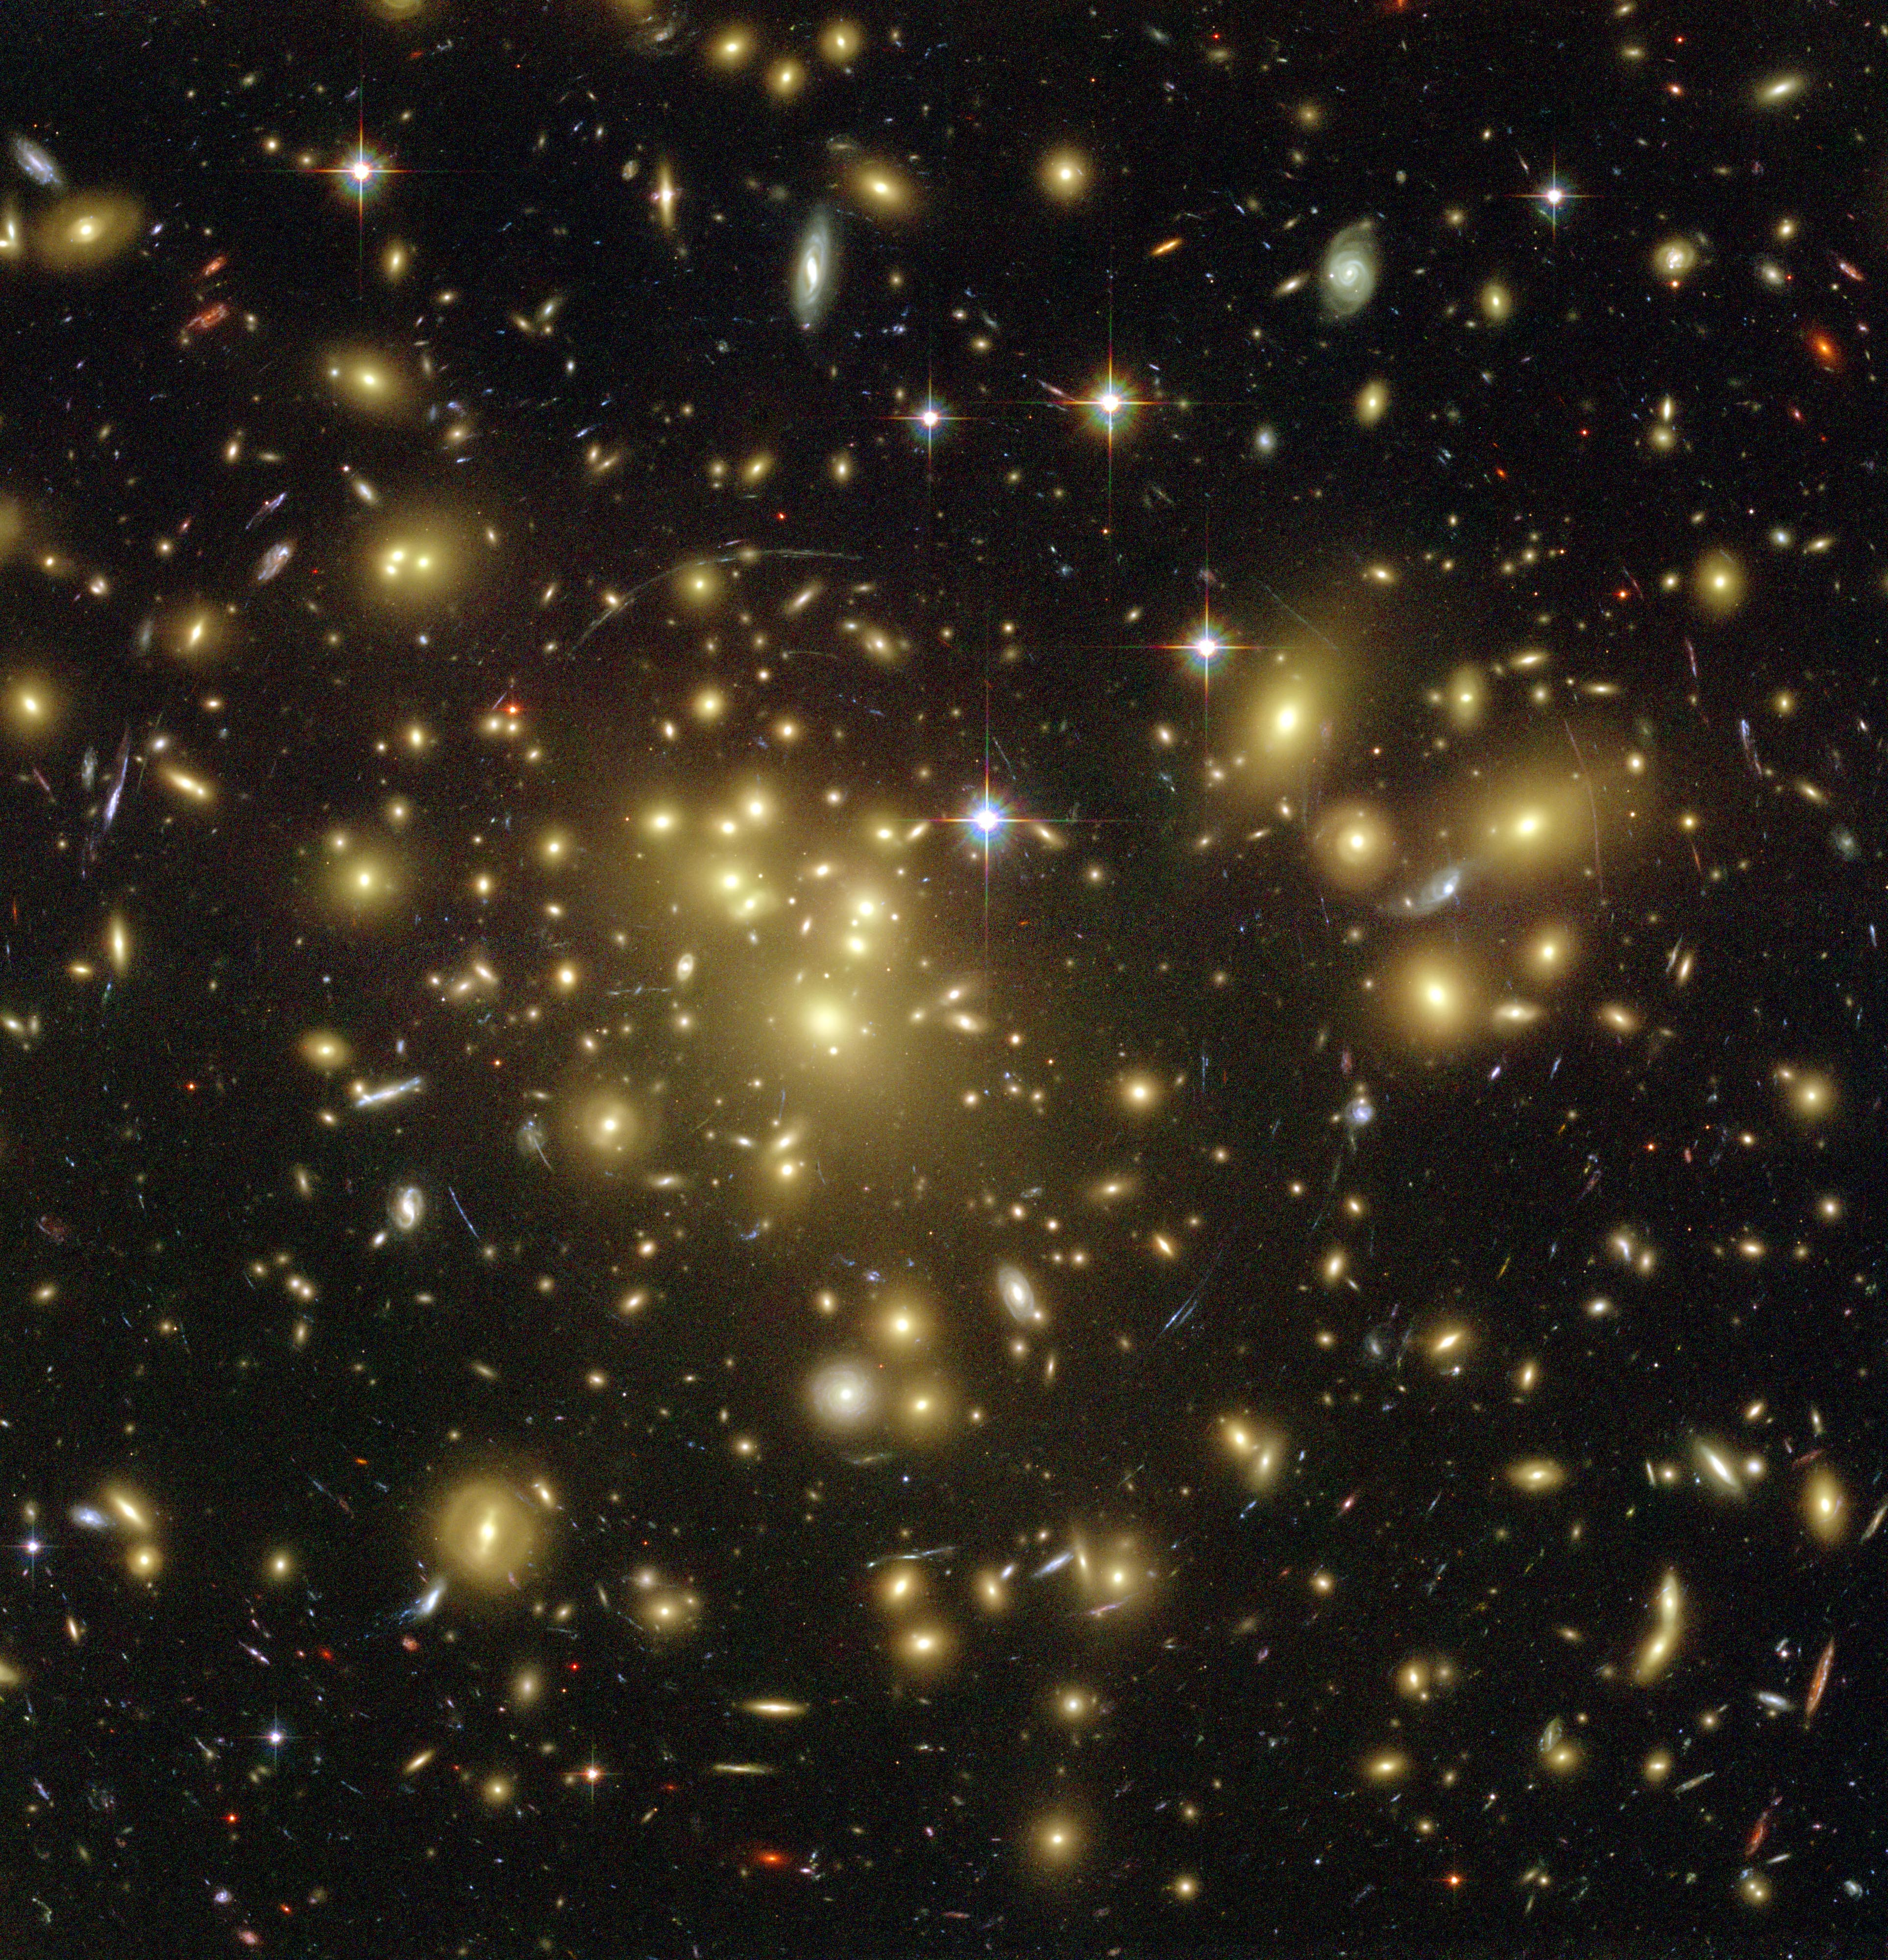
\includegraphics[height=\textheight]{abell-1689-hubble.jpg}
            \end{center}
            {\tiny HST/NASA}

    
}

\frame
{

    \frametitle{Dark Matter Correlation Function}

    \setbeamerfont*{itemize/enumerate body}{size=\small}

    \begin{columns}
        \begin{column}{0.5\textwidth}
            \begin{itemize}

                \item The lensing from foreground masses
                    causes correlations in the ellipticities

                \item Recall, the theory predicts the correlation function of
                    dark matter {\color{gold} $\langle \rho(\vec{r_1}) \rho(\vec{r_2})
                    \rangle$ }

                \item We can measure the correlation function in the
                    ellipticity {\color{gold} $\langle e(\vec{\theta_1})
                    e(\vec{\theta_2}) \rangle$ }

                \item The two correlation functions are intimately related

            \end{itemize}

        \end{column}
        \begin{column}{0.5\textwidth}
            \begin{center}
                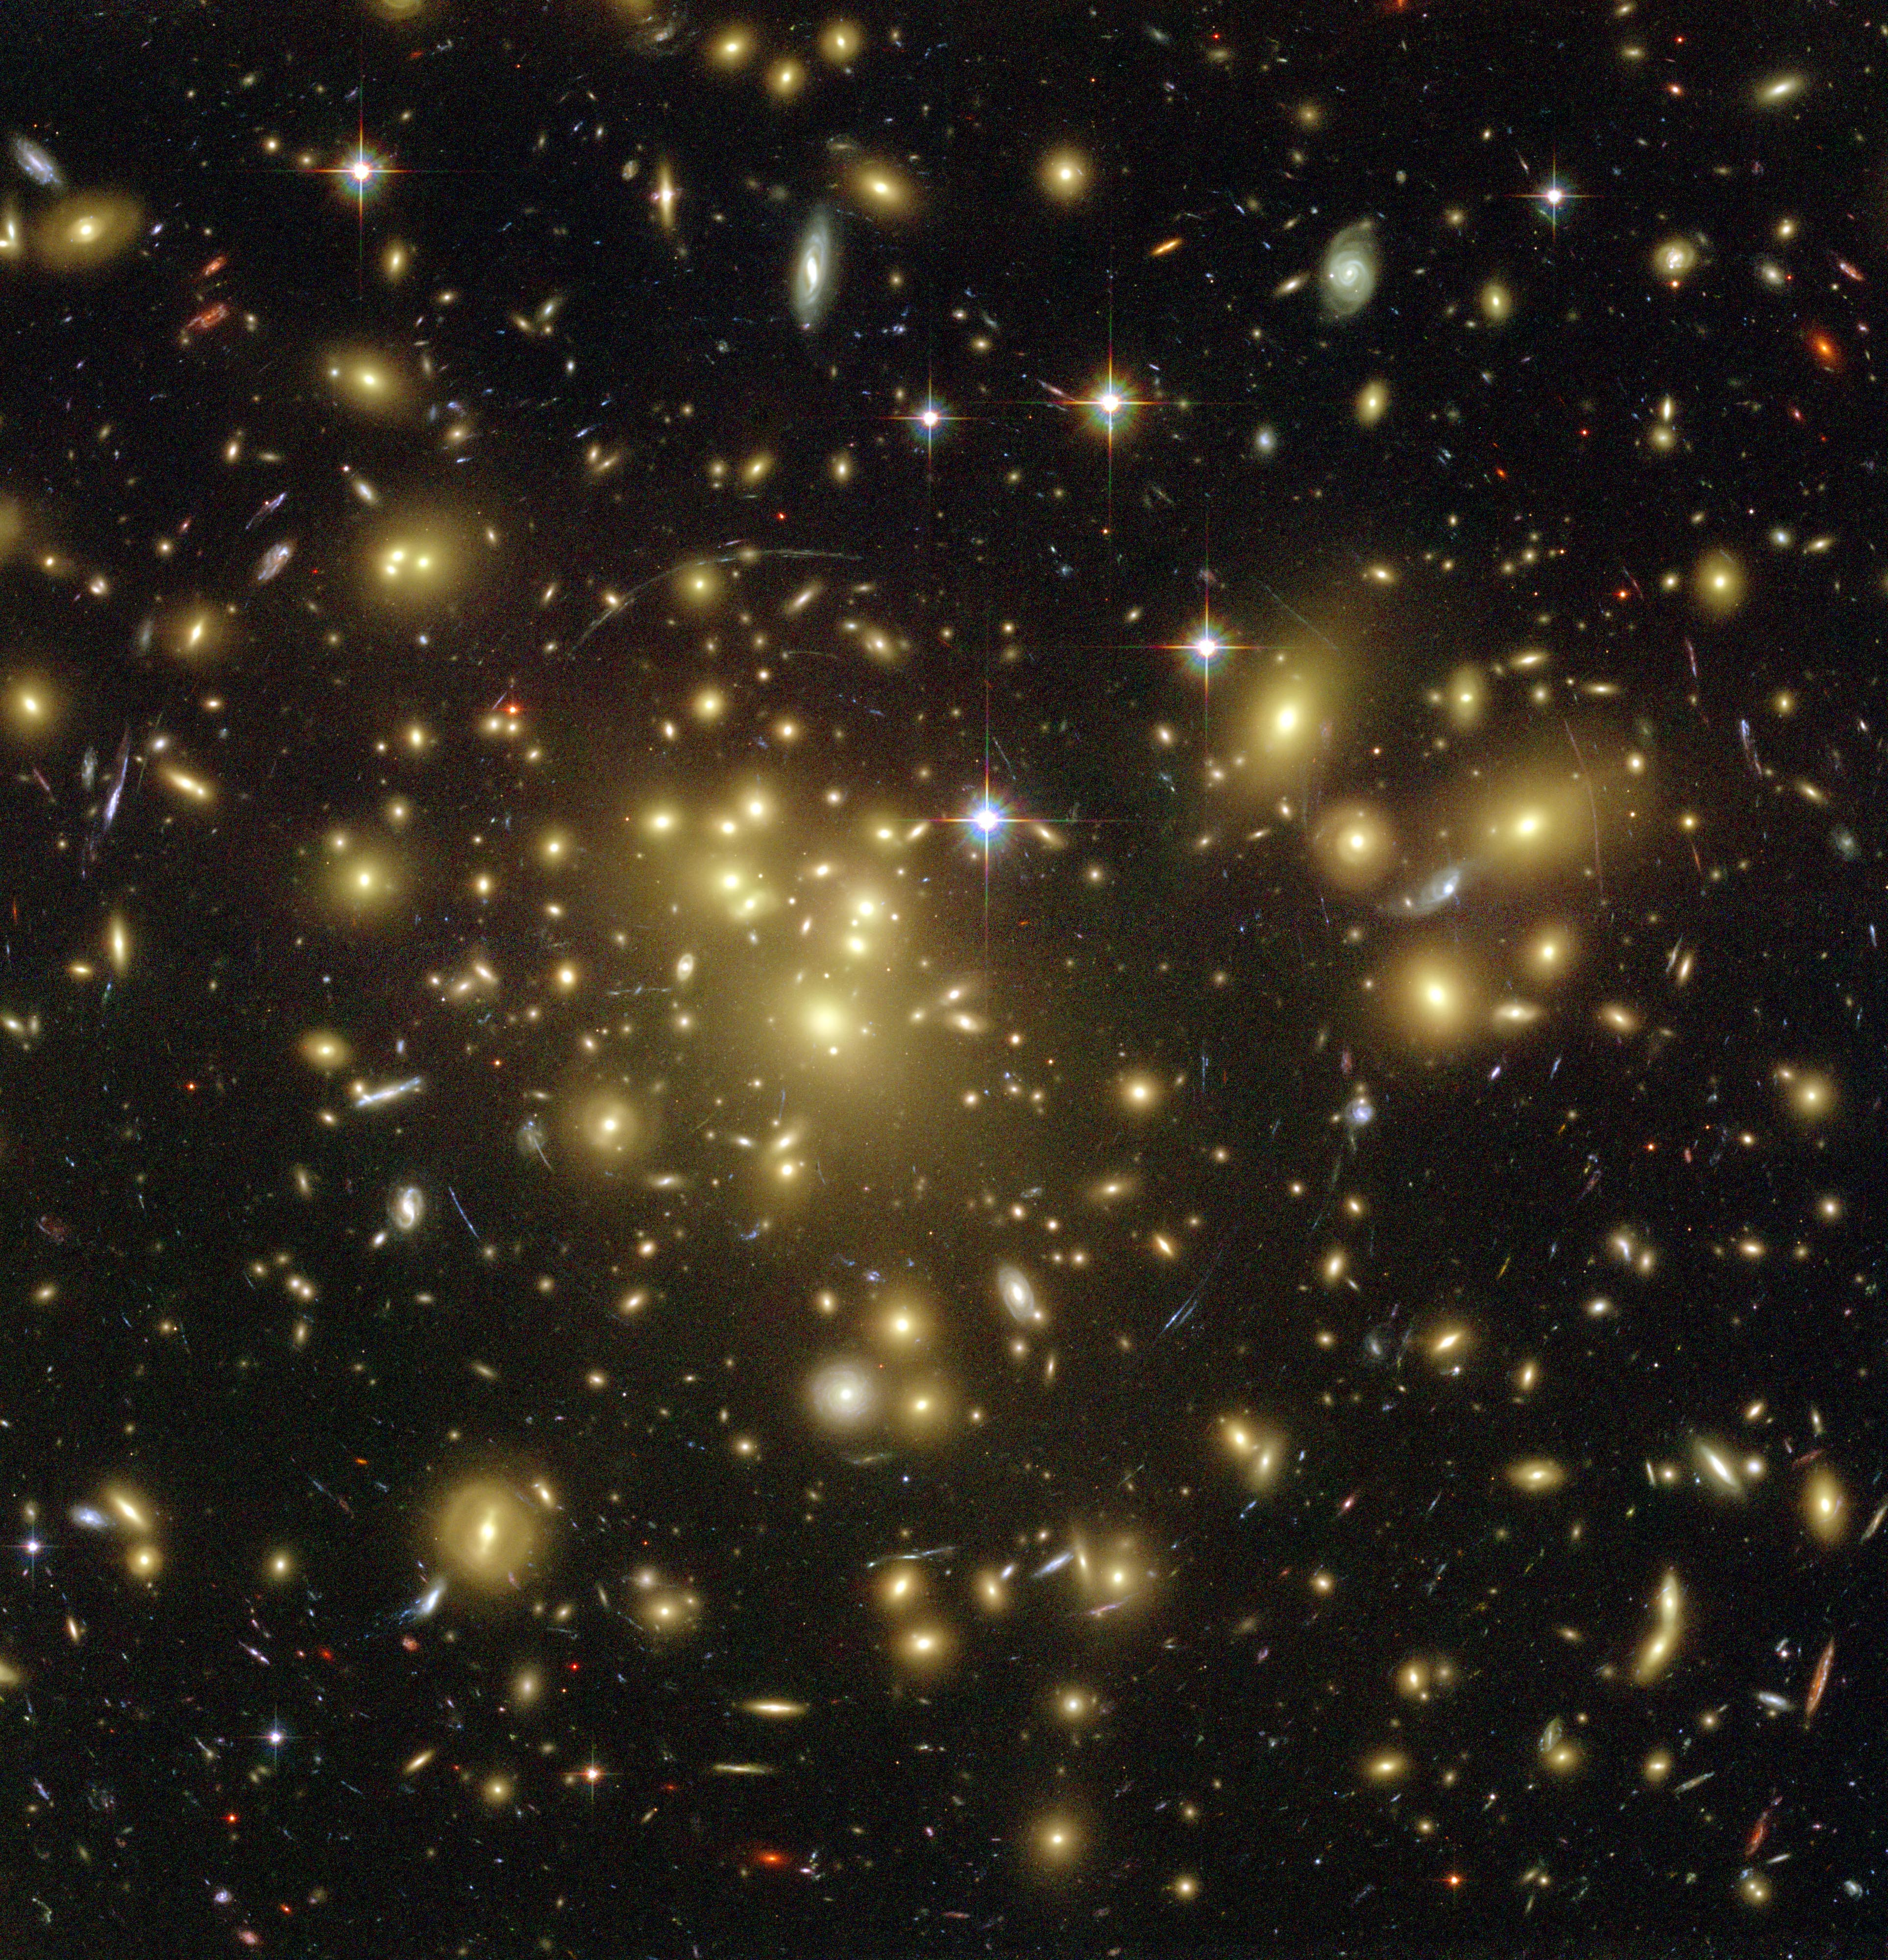
\includegraphics[width=\textwidth]{abell-1689-hubble.jpg}
                \newline
                {\tiny HST/NASA}
            \end{center}
        \end{column}

    \end{columns}


}

\frame
{

    \frametitle{Measuring Shear Correlation Function}

    \setbeamerfont*{itemize/enumerate body}{size=\small}

    \begin{columns}
        \begin{column}{0.5\textwidth}
            \begin{enumerate}

                \item Find Objects

                \item Measure sizes and brightness, statistically infer redshifts from
                    images through different color filters
                    
                \item Measure ellipticities

                \item Correct for blurring by atmosphere and telescope

                \item Measure the correlation function
                    {\color{gold} $\langle e(\vec{\theta_1}) e(\vec{\theta_2}) \rangle$ }



            \end{enumerate}

            After 30 years we now have an algorithm to calibrate
                this measurement accurately (Sheldon \& Huff 2017)

        \end{column}
        \begin{column}{0.5\textwidth}

            \begin{center}
                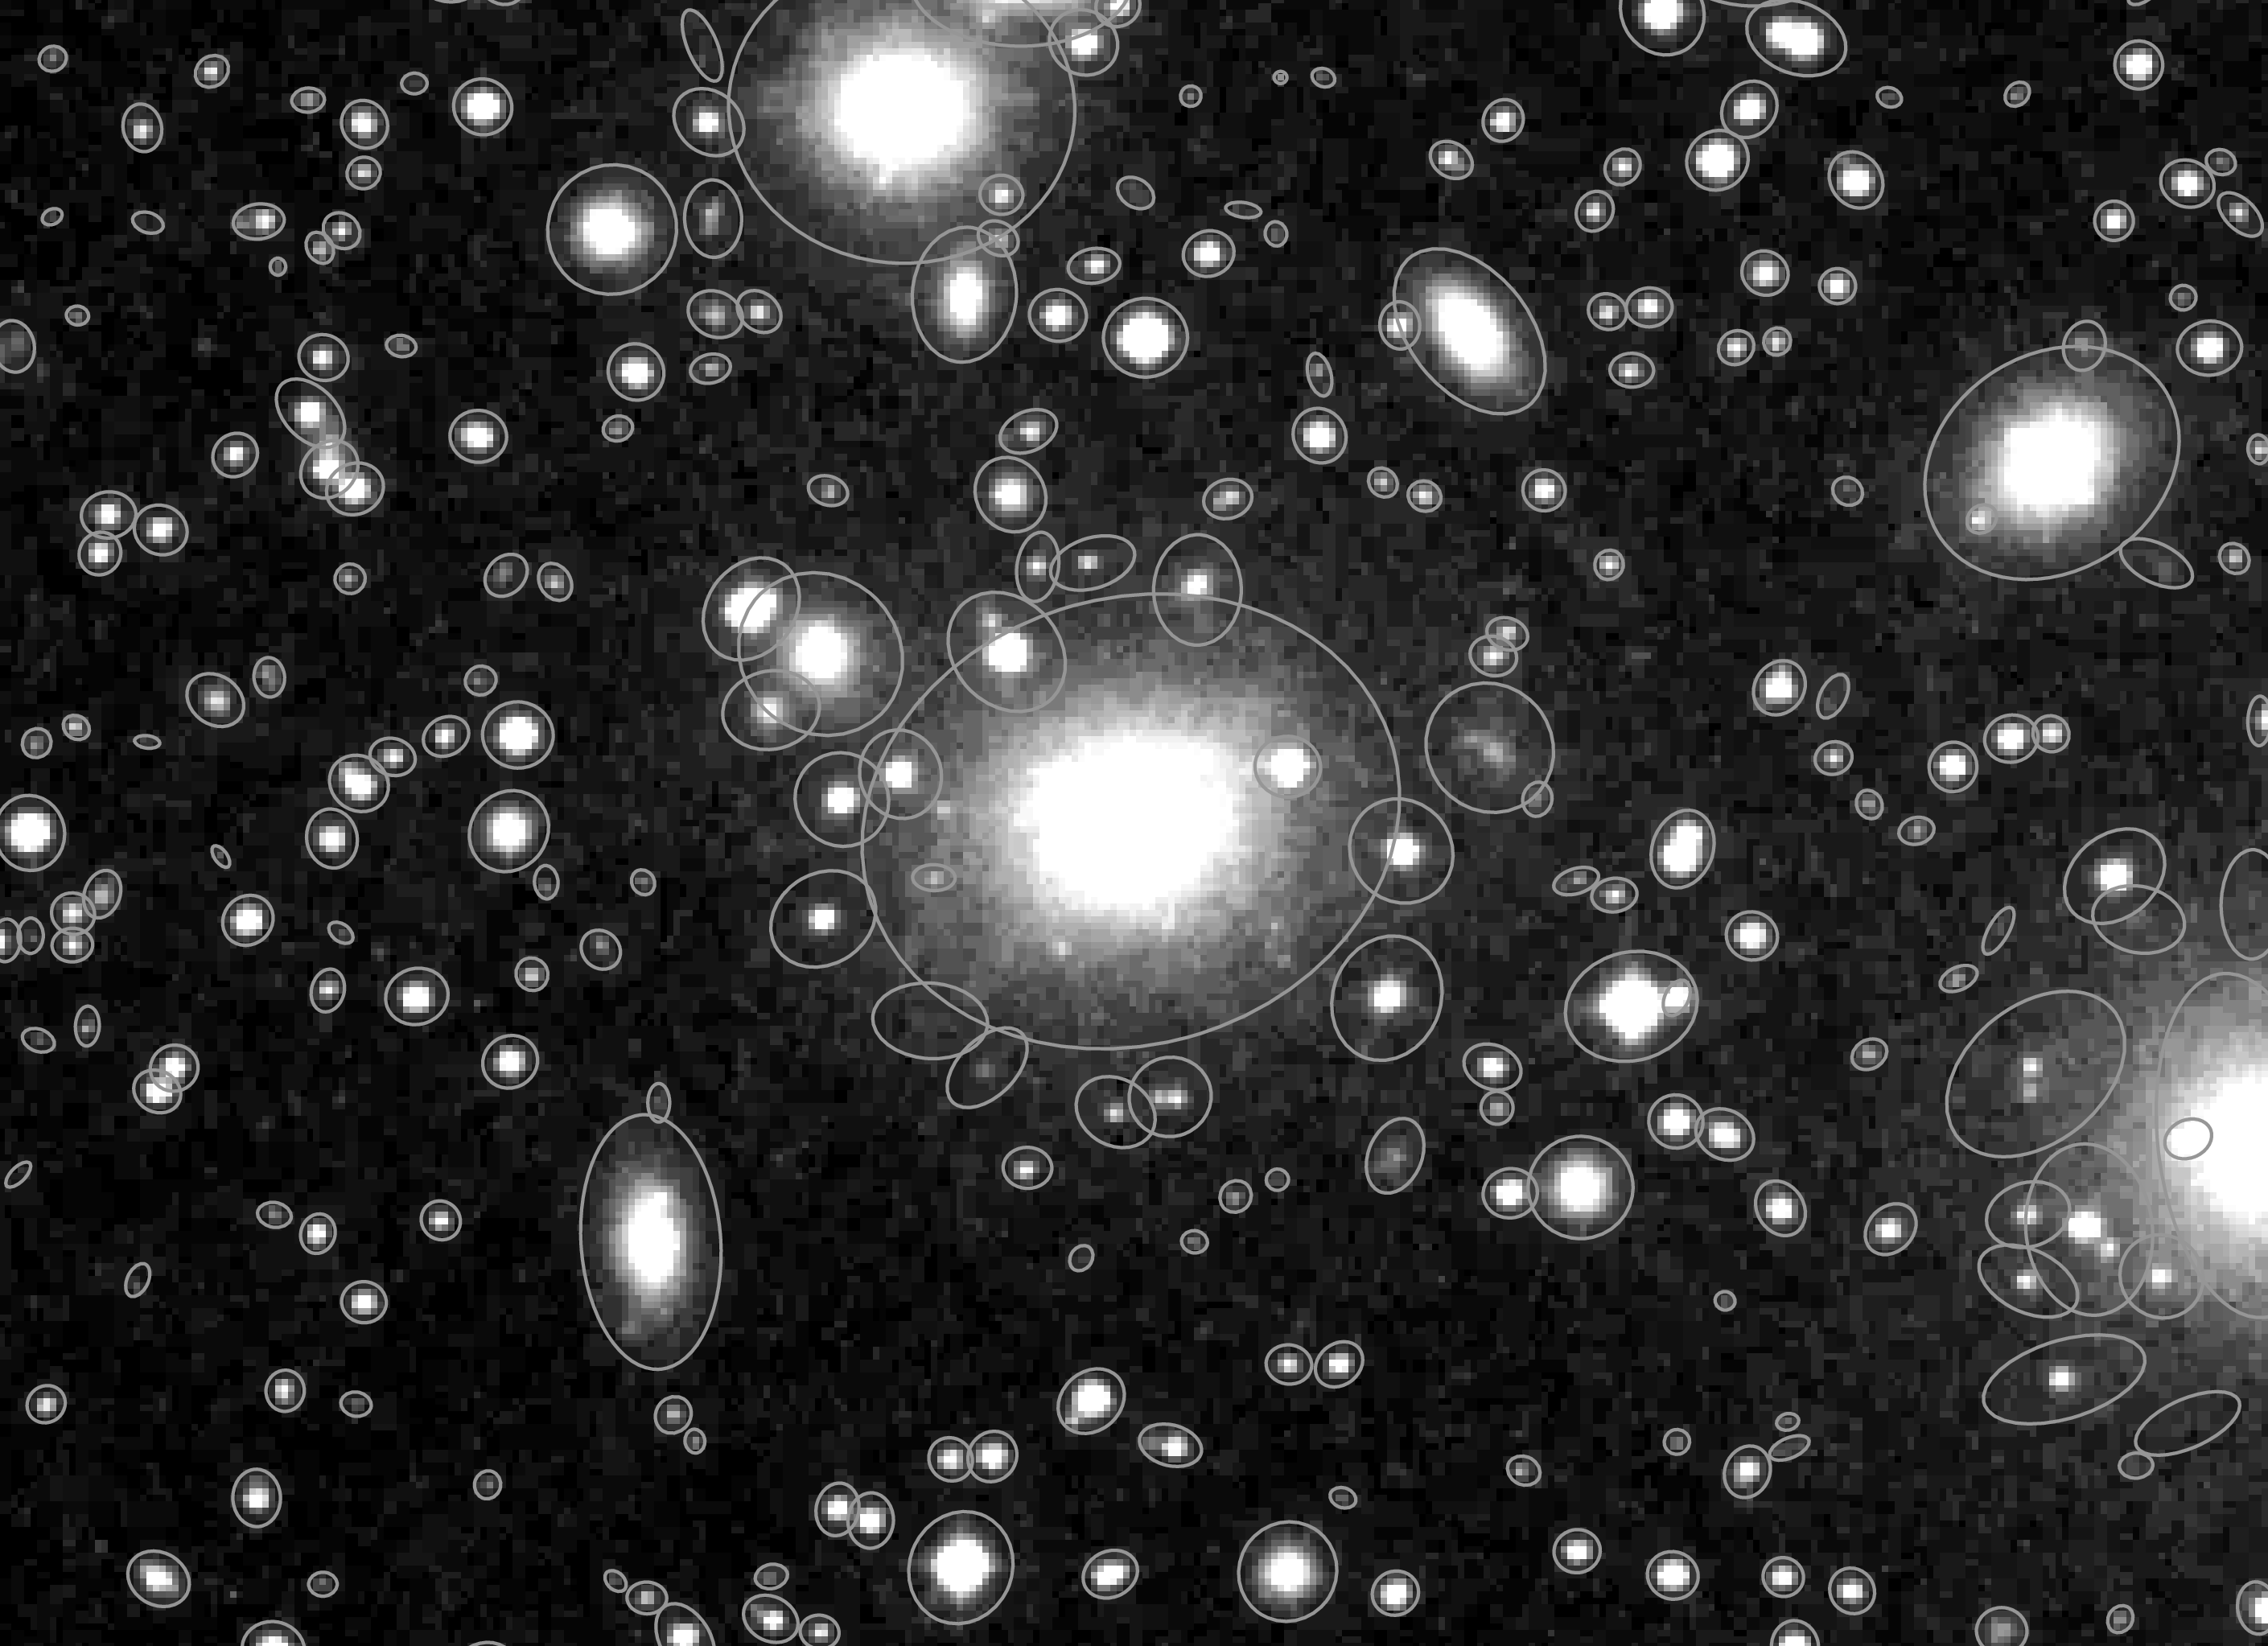
\includegraphics[width=\textwidth]{sun226_fig.png}
                \newline
                {\tiny Source Extractor (Bertin)}
            \end{center}

        \end{column}

    \end{columns}


}



\frame
{

    \frametitle{Weak Lensing Shear Correlation Function}

    \setbeamerfont*{itemize/enumerate body}{size=\small}

    \begin{columns}
        \begin{column}{0.5\textwidth}
            \begin{itemize}

                \item Best measurement to date is from CFHT survey

                \item Not yet very constraining

                \item Dark Energy Survey (DES) results will come out soon
                    
                \item DES measurments will be the first lensing results to place good
                    constraints on Dark Energy


            \end{itemize}

        \end{column}
        \begin{column}{0.5\textwidth}
            \begin{center}
                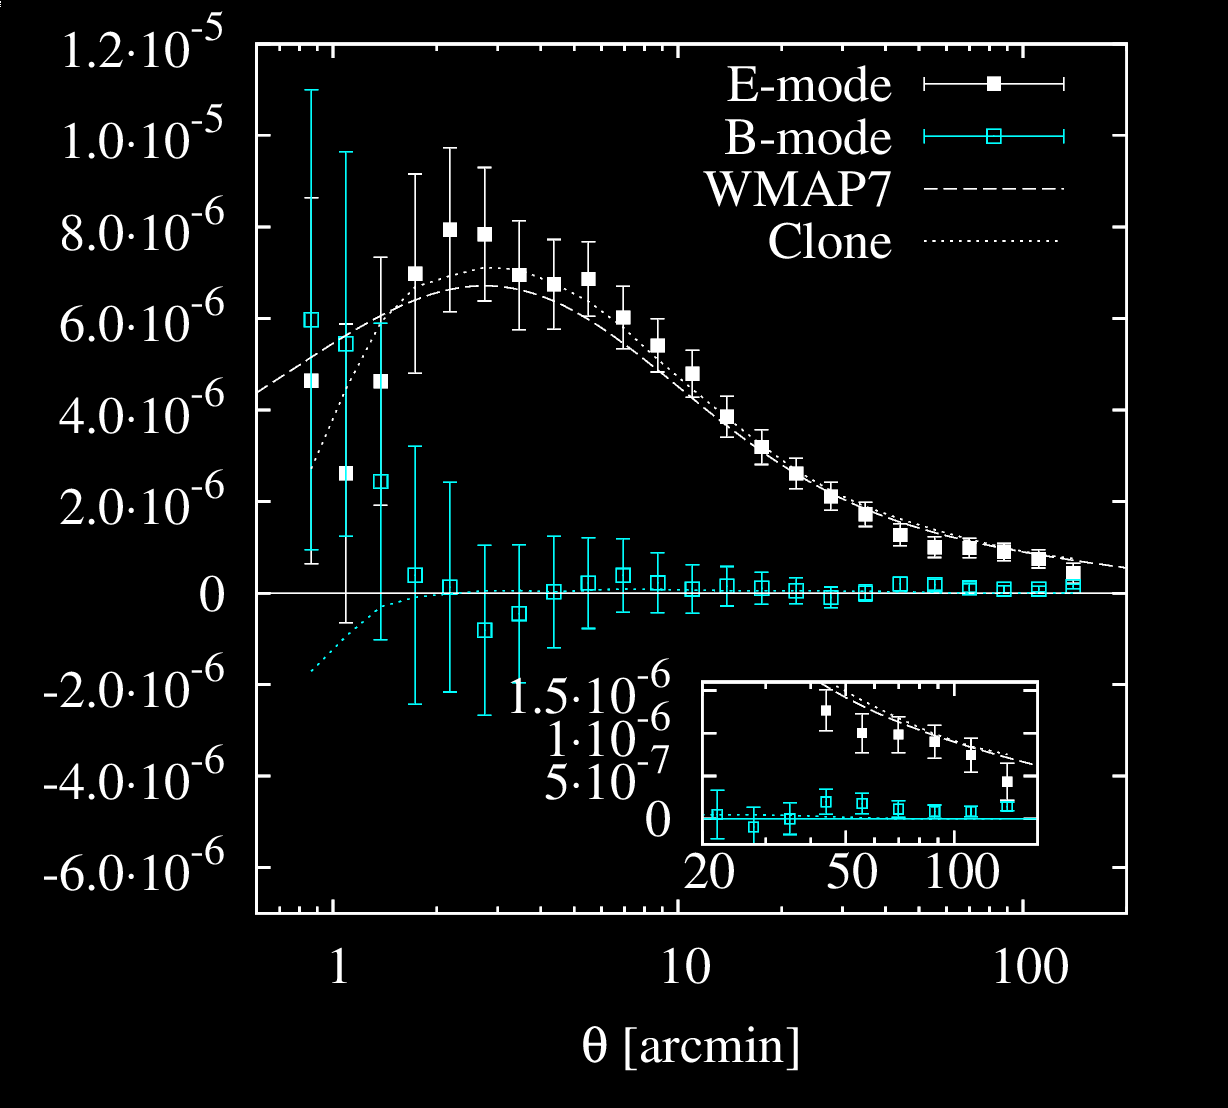
\includegraphics[width=\textwidth]{map-inv.png}
                \newline
                {\tiny CFHT}
            \end{center}
        \end{column}

    \end{columns}


}

\frame
{

    \frametitle{Summary}

    \setbeamerfont*{itemize/enumerate body}{size=\large}

    \begin{columns}
        \begin{column}{0.5\textwidth}
            \begin{itemize}

                \item With optical astronomy we can measure many of the
                    most direct predictions of our theory

                \item It all starts with pictures

                \item Expect exciting results in the near future

            \end{itemize}

        \end{column}
        \begin{column}{0.5\textwidth}
            \begin{center}
                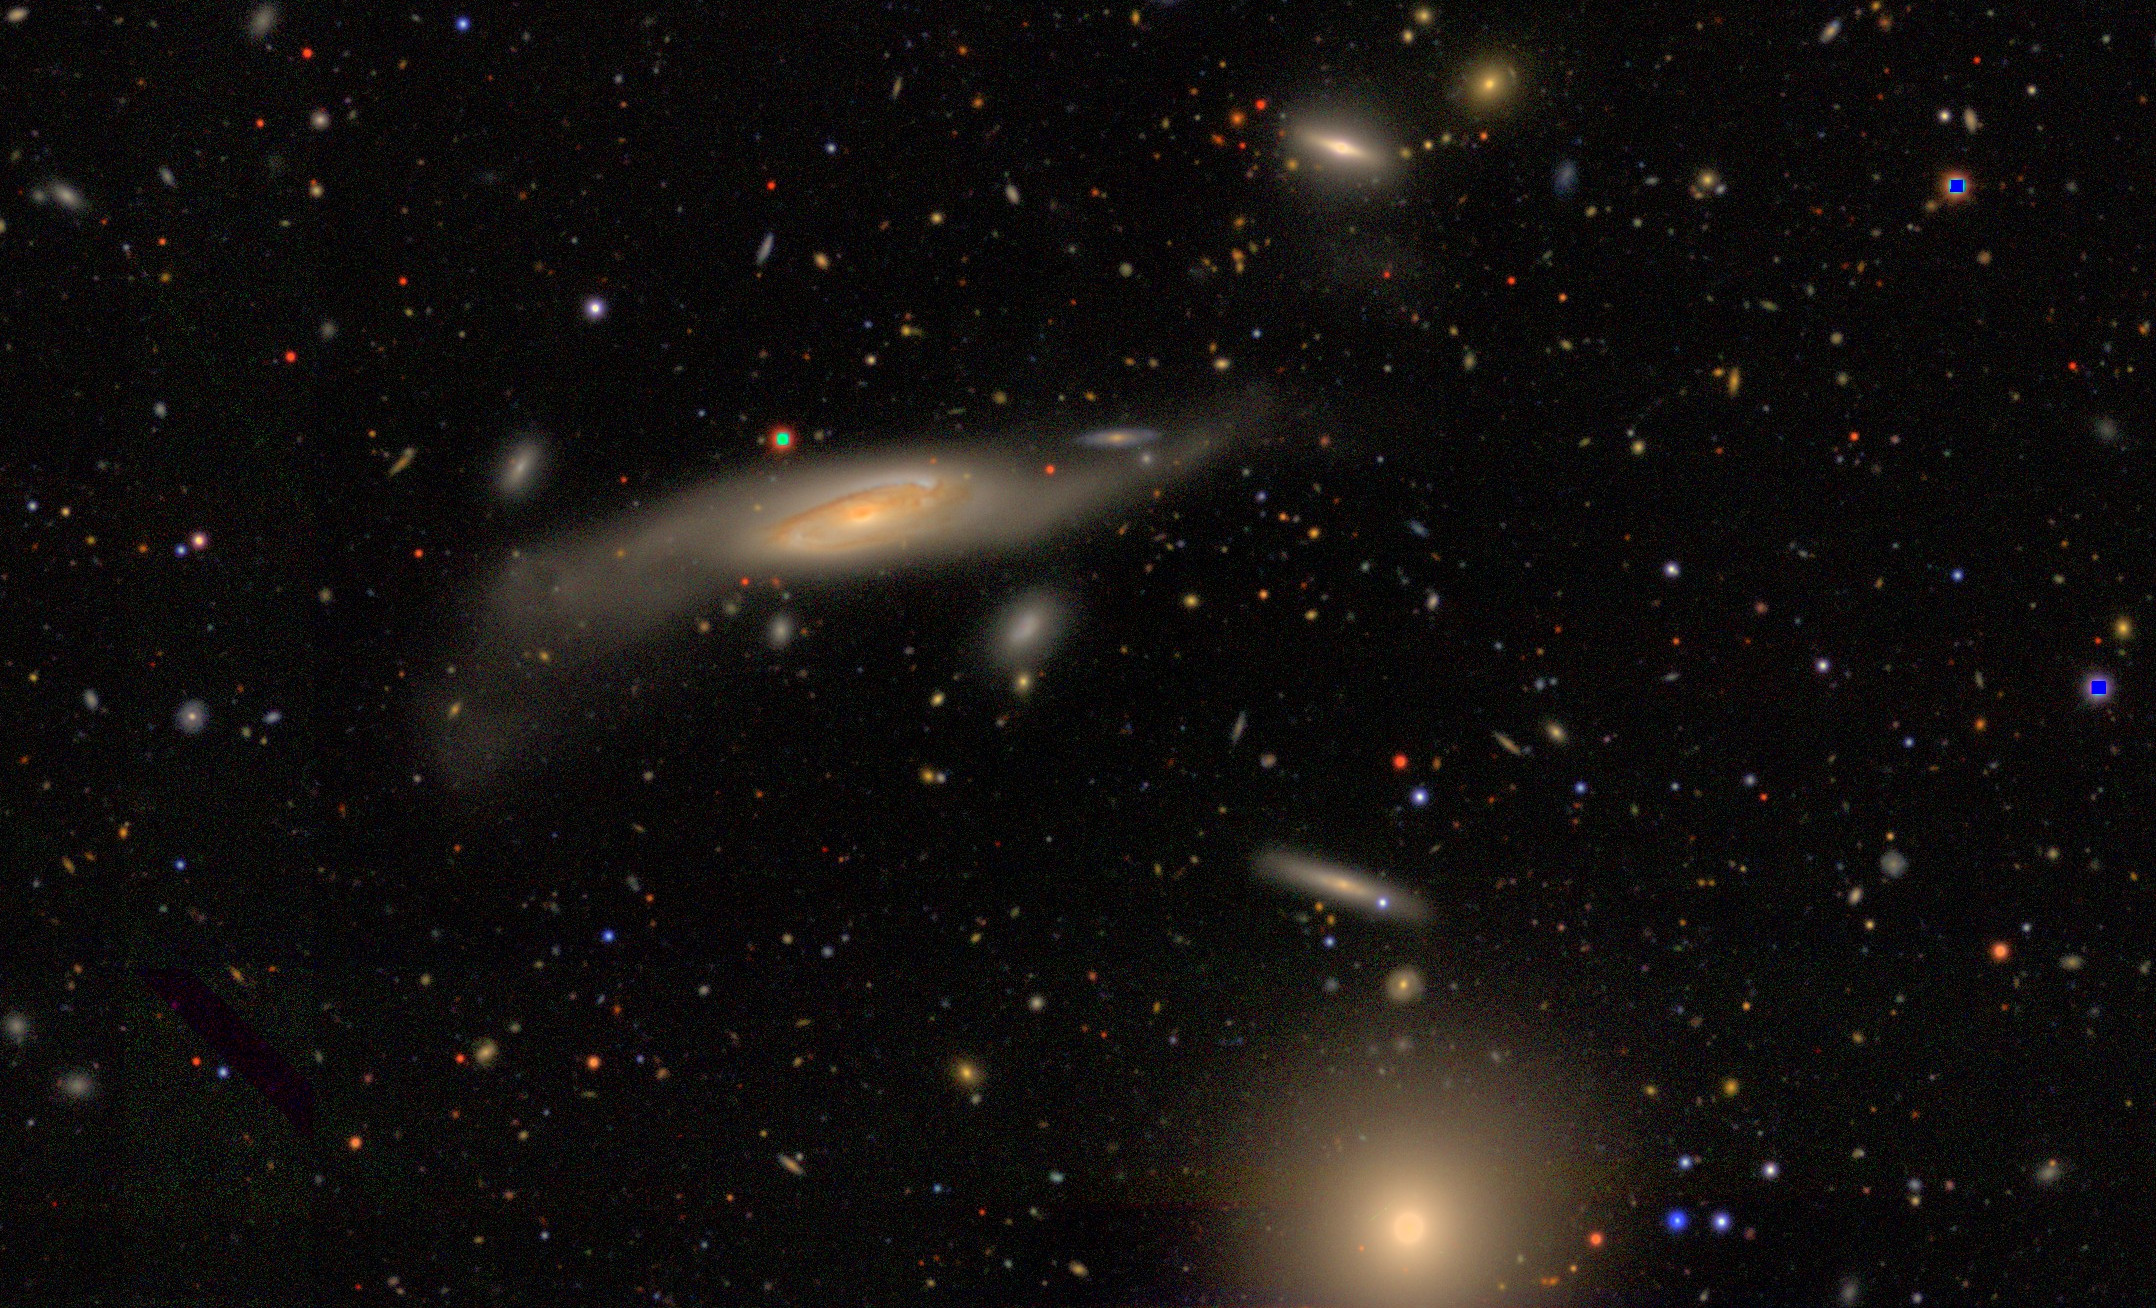
\includegraphics[width=1.2\textwidth, angle=90]{DES0056-5248_gri_crop.jpg}
                \newline
                {\tiny DES/Erin Sheldon}
            \end{center}
        \end{column}

    \end{columns}


}



\end{document}
